\documentclass[11pt]{article}
% Shared preamble for paper/main.tex and the appendix fragments.
\usepackage[utf8]{inputenc}
\usepackage[T1]{fontenc}
\usepackage{lmodern}
\usepackage{amsmath,amssymb,amsthm,mathtools}
\usepackage{graphicx}
\usepackage{booktabs}
\usepackage{enumitem}
\usepackage[margin=1in]{geometry}
\usepackage[colorlinks=true,linkcolor=blue,citecolor=blue,urlcolor=blue]{hyperref}

\newtheorem{lemma}{Lemma}[section]
\newtheorem{theorem}[lemma]{Theorem}
% Named results of the main text (Theorem A, Lemma 1, ...): unnumbered, with fixed names.
\newtheorem*{thmA}{Theorem A (strict plank bound)}
\newtheorem*{thmB}{Theorem B (constructions)}
\newtheorem*{corC}{Corollary C}
\newtheorem*{thmD}{Theorem D (small $n$)}
\newtheorem*{thmE}{Theorem E (random points)}
\newtheorem*{lemOne}{Lemma 1 (Bang's sign argument with a norm)}
\newtheorem*{corOne}{Corollary 1$'$ (Bang is never attained)}
\newtheorem*{lemTwo}{Lemma 2 (flat clusters)}
\newtheorem*{corTwo}{Corollary 2$'$ (restricted additive $2$-bases)}
\newtheorem*{propThree}{Proposition 3}
\newtheorem{proposition}[lemma]{Proposition}
\newtheorem{corollary}[lemma]{Corollary}
\newtheorem{claim}[lemma]{Claim}
\theoremstyle{definition}
\newtheorem{definition}[lemma]{Definition}
\theoremstyle{remark}
\newtheorem{remark}[lemma]{Remark}

\newcommand{\R}{\mathbb{R}}
\newcommand{\Z}{\mathbb{Z}}
\newcommand{\Q}{\mathbb{Q}}
\newcommand{\N}{\mathbb{N}}
\newcommand{\E}{\mathbb{E}}
\renewcommand{\Pr}{\mathbb{P}}
\newcommand{\ball}{B}                 % \ball^d = closed unit ball
\newcommand{\Sph}{S}                  % \Sph^{d-1} = unit sphere
\newcommand{\eps}{\varepsilon}
\newcommand{\abs}[1]{\left|#1\right|}
\newcommand{\norm}[1]{\left\|#1\right\|}
\newcommand{\ip}[2]{\langle #1,#2\rangle}
\DeclareMathOperator{\dist}{dist}
\DeclareMathOperator{\Var}{Var}
\DeclareMathOperator{\lcm}{lcm}
\DeclareMathOperator{\area}{area}
\DeclareMathOperator{\vol}{vol}
\DeclareMathOperator{\spn}{span}
\DeclareMathOperator{\adj}{adj}
\newcommand{\todoref}{\textbf{[TODO verify ref]}}


\title{Planks through points: covering a ball by slabs\\ around spanned hyperplanes}
\author{Michael Werman}
\date{Draft, \today}

\begin{document}
\maketitle

\begin{abstract}
Let $P$ be a set of $n$ points in the unit ball $\ball^d$, consider the hyperplanes spanned by its
affinely independent $d$-subsets, and write $K=\binom nd$. Let $\lambda_d(n)$ be the infimum, over all such
$P$, of the least $\eps$ for which the $\eps$-slabs around these hyperplanes cover the ball. Bang's plank
theorem gives $K\lambda_d(n)\ge1$, and freely placed hyperplanes attain this bound. We prove that for
$n>d$ spanned hyperplanes never attain it, and that they lose a constant factor in every dimension:
$\liminf n^d\lambda_d(n)\ge d!\,(1+q_d)$ with an explicit $q_d>0$. The proof integrates a quadratic test
function against a measure built from $3$-dimensional sphere sections. Conversely, clusters whose
hyperplane directions are sums of $d$ angles taken from restricted additive bases of cyclic groups give
$\lambda_d(n)=\Theta(n^{-d})$. As a by-product, restricted additive $2$-bases of cyclic groups with $n$
elements exist with modulus $(7/18-o(1))n^2$, which, to the best of our knowledge, improves the published
constants $5/18$ (restricted) and $1/3$ (unrestricted). For $n$ random points in a convex body $\Omega\subset\R^d$,
$n^d\rho/\log n$ converges in probability to an explicit constant $c_\Omega$ ($9\pi^2/8$ for the disc), so random sets lose
a logarithmic factor.
We also show that $2.1714\le\liminf n^2\lambda_2(n)$ and $\limsup n^2\lambda_2(n)\le9\pi/7$, that the centred square and the regular hexagon beat shrinking clusters
for $n=4$ and (with a computer-assisted bound) $n=6$, and we treat great hyperspheres, points anywhere in $\R^d$, flats spanned by $j+1$
points, and general convex bodies.
\end{abstract}

\section{Results}\label{sec:results}

For $P\subset\ball^d$ with $|P|=n$, let $\mathcal H_P$ be the set of hyperplanes through $d$ affinely
independent points of $P$, and
\[
K=\binom nd,\qquad \rho(P)=\max_{x\in \ball^d}\,\min_{H\in\mathcal H_P}\dist(x,H),\qquad
\lambda_d(n)=\inf_{|P|=n}\rho(P).
\]
Here $\rho(P)=\infty$ if $P$ has no $d$ affinely independent points, and $n\ge d$ throughout. Several
$d$-subsets may span the same hyperplane, and dependent $d$-subsets span none, so $\mathcal H_P$ has
$K'\le K$ elements; the proofs write $N_H\ge1$ for the number of independent $d$-subsets lying in
$H\in\mathcal H_P$.

For comparison, if the $\eps$-slabs around any $k$ hyperplanes cover $\ball^d$, then $\eps\ge1/k$ (Bang
\cite{Bang}); if the hyperplanes all pass through the centre, then $\eps\ge\sin(\pi/2k)$ (the zone theorem
of Jiang and Polyanskii \cite{JP}, in Zhao's form \cite{Zhao}). Equality is attained by $k$ parallel,
equally spaced hyperplanes in the first case, and by $k$ hyperplanes through a common $(d-2)$-flat
through the centre at successive angles $\pi/k$ in the second.

\begin{thmA}
For $d\ge2$ and $n\ge d$, every $n$-point set $P\subset\ball^d$, with $\rho=\rho(P)$, satisfies
\[
\binom nd\,\rho\ \ge\ \frac{1+q_d}{1+2\rho/A_d},\qquad A_d=\frac{3d-1}{d-1},\qquad
q_d=\min_{|m|\le1}\frac{1/3+m^2}{\Lambda_d(m)},
\]
where $\Lambda_2=A_2$ and, for $d\ge3$,
$\Lambda_d(m)=A_d+(1+|m|)^2(C_d-1)+4(1+|m|)\tfrac{d-3}{d-1}$
with $C_d=\sqrt\pi\,\Gamma(\tfrac{d-1}2)/\Gamma(\tfrac{d-2}2)$; since $C_3=1$, $\Lambda_3=A_3$.
\end{thmA}

So $q_2=1/15$ and $q_3=1/12$, and the bound reads $\binom n2\rho\ge 16/(15+6\rho)$ in the plane and
$\binom n3\rho\ge 13/(12+6\rho)$ in space; for $d\ge4$, $q_d\ge0.08/\sqrt{d-2}$, by hand: exact values of
$C_d$ for $4\le d\le7$, and for $d\ge8$ one quadratic in $m$ with negative discriminant, using
$C_d\le\sqrt{\pi(d-2)/2}$ (Appendix~\ref{sec:A-qd}). So
$\liminf n^d\lambda_d(n)\ge L_d:=d!\,(1+q_d)$, with $L_2=32/15$, $L_3=13/2$, $L_4\ge25.41$ and
$L_5\ge125.95$. For $d=2,3$ the exact position of the points on their hyperplanes gives larger limit constants:
$\binom n3\rho\ge70/(63+60\rho)$, so $\liminf n^3\lambda_3(n)\ge20/3$, and
$\liminf n^2\lambda_2(n)\ge6864/3161>2.1714$. Complete proofs are in Appendix~\ref{app:A}; the sharper
constants are in Appendix~\ref{sec:A-sharp}.

\begin{thmB}
For $n\ge d+1$, $\lambda_d(n)\le\sin(\pi/2p_d(n))$, where $p_d(n)$ is the largest $N$ such that some
$n$-subset of $\Z_N$ has every residue as a sum of $d$ distinct elements; $n\le p_d(n)\le\binom nd$.
More generally, $\lambda_d(n)\le\sin(G/2)$ whenever $G$ is the largest gap mod $\pi$ of the sums of $d$
distinct elements of some $n$ distinct $\theta$'s in $(0,\pi)$. Moreover,
$\sigma_d=\lim p_d(n)/n^d$ exists and equals $\sup_{n>d}p_d(n)/n^d\le 1/d!$.
\end{thmB}

\begin{corC}
$\lambda_d(n)=\Theta(n^{-d})$, since $\sigma_d=\sup p_d(n)/n^d\ge p_d(d+1)/(d+1)^d\ge(d+1)^{1-d}>0$ by
Theorem~B ($p_d(n)\ge n$); the examples in the table below yield stronger constants for $d\le5$. More
precisely, with $\ell_2=6864/3161$, $\ell_3=20/3$ and $\ell_d=L_d$ for $d\ge4$,
\[
\ell_d\;\le\;\liminf_{n\to\infty}n^d\lambda_d(n)\;\le\;\limsup_{n\to\infty}n^d\lambda_d(n)\;\le\;
\frac{\pi}{2\sigma_d}.
\]
\end{corC}

\begin{center}
\small
\begin{tabular}{p{4.3cm}cccc}
\toprule
$d$ & 2 & 3 & 4 & 5\\
\midrule
proved lower bound for $\liminf n^d\lambda_d(n)$ & $2.1714$ & $20/3$ & $25.41$ & $125.95$\\
upper bound $\pi n^d/(2N)\ge\pi/(2\sigma_d)$ & $9\pi/7\approx4.04$ & $100\pi/19\approx16.5$ &
$1024\pi/33\approx97.5$ & $5000\pi/21\approx748$\\
from the example $(n,N)$ & $(12,56)$ & $(10,95)$ & $(8,66)$ & $(10,210)$\\
\bottomrule
\end{tabular}
\end{center}

\begin{thmD}
In the plane, the centred square gives $\lambda_2(4)\le 1/\sqrt{10+4\sqrt2}\approx0.25272$, and the
regular hexagon gives $\lambda_2(6)\le1/\sqrt{56+16\sqrt3}\approx0.10930$. Both beat every cluster
shrinking to the centre: such clusters have a strictly larger $\liminf\rho$ (Figure~\ref{fig:square}; for $n=6$ this
uses the computer-assisted bound on $\gamma_6$ of Table~\ref{tab:gamma}).
\end{thmD}

Here $\gamma_n$ denotes the infimum, over $n$-point sets in the plane, of the largest gap mod $\pi$
between the directions of their spanned lines; a cluster shrinking to the centre has
$\rho\to\sin(G/2)$, with $G$ its own largest gap, so the best clusters give $\sin(\gamma_n/2)$. (If all spanned lines pass within $r$ of the centre, each
is within $r$ of a parallel line through the centre, so $\rho\ge\sin(G/2)-r$; hence clusters shrinking to
the centre have $\liminf\rho\ge\sin(\gamma_n/2)$.) The
same quantity appears, as $\rho_2(n)=\sin(\gamma_n/2)$, in Frankl and Maehara's work on projecting
finite point sets \cite{FM} (we have seen only the zbMATH review; the full text is not online). OEIS
A004131, the sequence $p_2(n)$, cites their paper, so they may already have used the link between chord
directions and restricted cyclic bases that underlies Theorem~B for $d=2$. We therefore claim that link
as new only for $d\ge3$, and even this claim rests on the review, not on the full text.

\begin{thmE}
Let $\Omega\subset\R^d$ ($d\ge2$) be a convex body and $X_1,\dots,X_n$ independent uniform points of
$\Omega$. The covering radius $\rho_\Omega=\max_{x\in\Omega}\min_H\dist(x,H)$, over the hyperplanes $H$ spanned by
$d$ of the points, satisfies $n^d\rho_\Omega/\log n\to c_\Omega=d^2\,d!/m_\Omega$ in probability. Here
$m_\Omega=\min_{z\in\Omega}h_\Omega(z)$, where $h_\Omega(z)=\lim_{t\to0}\Pr(\dist(z,H)<t)/t$ for the hyperplane $H$ through
$d$ independent uniform points of $\Omega$. In the plane
$c_\Omega=12|\Omega|^2/\min_{z\in\Omega}\int_0^\pi L_z(\theta)^3\,d\theta$, with $L_z(\theta)$ the chord through $z$ in direction
$\theta$; for the unit disc, $n^2\rho/\log n\to9\pi^2/8\approx11.10$.
\end{thmE}

Theorem~A, Corollary~1$'$ and the small-$n$ results use the ball; Section~\ref{sec:convex} says what extends to
other convex bodies.

\section{The lower bound}\label{sec:lower}

\begin{lemOne}
If the closed $\eps$-slabs around hyperplanes $\{\ip{x}{u_j}=m_j\}$ with $|u_j|=1$ cover $\ball^d$, then
$\eps\cdot\max_{|v|=1}\sum_j|\ip{u_j}{v}|\ge1$.
\end{lemOne}

\begin{proof}
For $\eps'>\eps$ choose signs $\sigma$ maximising $|x_\sigma|^2-2\eps'\sum\sigma_jm_j$, where
$x_\sigma=\eps'\sum\sigma_ju_j$. Flipping $\sigma_i$ changes this by
$-4\eps'[\sigma_i(\ip{x_\sigma}{u_i}-m_i)-\eps']\le0$. So $x_\sigma$ lies outside every slab, hence
outside the ball, and $1<|x_\sigma|\le\eps'\max_v\sum|\ip{u_j}{v}|$. Let $\eps'\downarrow\eps$. (This is
a one-line consequence of Bang's lemma as stated in Verreault's survey \cite{Verreault}, Lemma~2.5:
Bang's point avoids every slab, and its norm is at most $\eps'\max_v\sum|\ip{u_j}{v}|$.)
\end{proof}

\begin{corOne}
$\lambda_d(n)>1/\binom nd$ for every $d\ge2$ and $n>d$.
\end{corOne}

\begin{proof}
By Lemma~1, $\lambda_d(n)\ge1/K$. Suppose equality, and take labelled $n$-point sets $P_k$ with
$\rho(P_k)\to1/K$. Pass to a subsequence on which the family $I$ of independent $d$-sets is fixed, every
point converges, and for $F\in I$ the hyperplane $\{\ip{x}{u_F}=m_F\}$ ($|u_F|=1$, $|m_F|\le1$)
converges. If $|I|<K$, Lemma~1 gives $\rho(P_k)\ge1/(K-1)$ for all $k$, so $I$ consists of all $K$
$d$-sets. The covering radius of a finite list is $1$-Lipschitz in the $(u,m)$, so the limit list has
covering radius $1/K$, and its $F$-th member contains the limits of the points of $F$. By Lemma~1 with
$\eps=1/K$, some unit $v$ has $\sum_F|\ip{u_F}{v}|\ge K$, so every $u_F=\pm v$. The $K$ slabs of
half-width $1/K$ then cover the diameter in direction $v$ with total length $2$, so their offsets are
distinct. But the limit hyperplanes of $\{1,\dots,d\}$ and $\{2,\dots,d+1\}$ are both $\perp v$ and
contain the limit of $p_2$. (Details in Appendix~\ref{sec:A-strict}.)
\end{proof}

Theorem~A makes this quantitative once $\binom nd>2/(q_dA_d)$: then
\[
\lambda_d(n)\ge\frac{A_d}{4}\Bigl(\sqrt{1+8(1+q_d)\big/\bigl(A_d\tbinom nd\bigr)}-1\Bigr)>1\Big/\tbinom nd.
\]

Applied to $\mathcal H_P$, Lemma~1 shows that if $\rho(P)$ is close to Bang's bound $1/K$, then the
normals are nearly parallel. To quantify this, fix the maximising $v$, orient the normals so that
$\cos\psi_H=\ip{u_H}{v}\ge0$, and define the height of $x$ as $t(x)=\ip{x}{v}$. With $\eps=\rho(P)$, Lemma~1 gives $\sum_{H\in\mathcal H_P}\cos\psi_H\ge1/\eps$, so
$\sum_{H\in\mathcal H_P}(1-\cos\psi_H)\le K-1/\eps$. If $N_H$ $d$-subsets lie on $H$, then
$N_H(1-\cos\psi_H)\le(1-\cos\psi_H)+(N_H-1)$; adding the dependent $d$-sets gives the \emph{tilt
budget}
\[
\sum_{\text{independent }Q}(1-\cos\psi_Q)\;+\;\#\{\text{dependent }d\text{-sets}\}\;\le\;K-\frac1\eps.
\]

\begin{proof}[Proof of Theorem A (outline; the full proof is Appendix~\ref{sec:A-unified})]
Let $\eps=\rho(P)$, let $m_0$ be the mean height of the points, and integrate $\Phi(x)=(t-m_0)^2$
against a measure whose height is uniform on $[-1,1]$, so that $\int\Phi=1/3+m_0^2$. For $d=2$ take the
Archimedes measure $dx/(2\pi\sqrt{1-|x|^2})$ (Gardner's relative-width measure of the disc
\cite{Gardner}), and for $d\ge3$ the uniform measure on $\Sph^{d-1}\cap V$ averaged over random
$3$-spaces $V\ni v$ ($V=\R^3$ when $d=3$). Dimension $3$ is forced by the method: only on the
$2$-sphere is the height of a uniform point uniform (Archimedes); on a circle it has the arcsine law,
whose density is unbounded at $\pm1$, so a slab of half-width $\eps$ near a pole can carry mass of order
$\sqrt\eps$ rather than $\eps$.
\begin{enumerate}
\item \textbf{One slab.} On a section circle at offset $s$ and tilt $\psi$ the mean of $\Phi$ is
$G(s)=(s\cos\psi-m_0)^2+\sin^2\psi\,(1-s^2)/2$ (for $d=2$, pull the slab and $\Phi$ back to
$\Sph^2$ by the projection). Since $|m_0|,|m_H|\le1$, $|G'|\le(1+\cos\psi)^2\le4$ on $[-1,1]$, so
the slab of $H$ carries $\Phi$-mass at most $\eps[G_H(m_H)+e(\psi_H)]+2\eps^2$, with $e=0$ for
$d\le3$. For $d\ge4$ write $u_H=\cos\psi\,v+\sin\psi\,e_H$; the slab meets $V$ in a slab of half-width
$\eps/r$, where $r=\sqrt{\cos^2\psi+\beta\sin^2\psi}$ and $\beta=|P_Ve_H|^2$ has law
$\mathrm{Beta}(1,\frac{d-3}2)$, so $\E\beta=2/(d-1)$ and $\E\beta^{-1/2}=C_d$. The section circles have
tilt $\arccos(\cos\psi/r)$ and centres moved in height by at most $1-r^2$, with
$\E(1-r^2)=\frac{d-3}{d-1}\sin^2\psi$; and
$\E[1/r]-1\le(C_d-1)(1-\cos\psi)$ (the ratio is largest for $\psi=\pi/2$, by a monotonicity argument: Lemma~R in Appendix~\ref{sec:A-unified}).
Together these give $e(\psi)\le(\Lambda_d(m_0)-A_d)(1-\cos\psi)$: steep slabs carry more mass, but they
also spend more of the tilt budget.
\item \textbf{$d$-sets.} For a $d$-set $Q$ on $H$, put $X=(\text{mean height of }Q)-m_0$ and
$Y=(\text{foot height of }H)-(\text{mean height of }Q)$, and let $\Var$ be the mean squared deviation of
the heights in $Q$. Then $Y^2+\Var\le W^2:=\sin^2\psi\,(1-m_H^2)$, and over all $d$-sets
$\sum X^2=\frac{n-d}{(d-1)n}\sum\Var$: mean heights cannot all sit near $m_0$ unless the $d$-sets are
spread out. For each $H$ choose one independent $d$-set $Q\subset H$; by Cauchy--Schwarz and $Y^2\le W^2-\Var$,
$G_H(m_H)=(X+Y)^2+W^2/2\le dX^2+\frac d{d-1}(W^2-\Var)+W^2/2$. Sum this over all independent
$d$-sets. The identity bounds $d\sum X^2$ by $\frac d{d-1}\sum\Var$, both over all $d$-sets, so the $X^2$
terms cancel against the $-\Var$ terms up to $\frac d{d-1}\#\{\text{dependent }d\text{-sets}\}$ (as
$\Var\le1$). With $W^2\le2(1-\cos\psi)$ and the tilt budget, $\sum_HG_H\le A_d(K-1/\eps)$.
\item \textbf{Conclusion.} Summing over $H$ with the tilt budget, covering gives
$1/3+m_0^2\le\Lambda_d(m_0)(K\eps-1)+2K\eps^2$, that is
$K\eps\ge(1+I/\Lambda)/(1+2\eps/\Lambda)\ge(1+q_d)/(1+2\eps/A_d)$, with $I=1/3+m_0^2$ and
$\Lambda=\Lambda_d(m_0)\ge A_d$. As $x\mapsto x(1+2x/A_d)$ is continuous and increasing, the bound
passes to the infimum $\lambda_d(n)$, which gives the liminf.\qedhere
\end{enumerate}
\end{proof}

\paragraph{Sharper constants for $d=2,3$.} Step~2 relaxes the position of the points of $Q$ to
$Y^2+\Var\le W^2$. In fact every point of $Q$ has height within $W$ of the foot height of $H$, and
$(d-1)X^2-\Var=\frac2d\sum_{i<j}x_ix_j$ in the centred heights $x_i$, which is affine in each $x_i$; so
for a per-$d$-set inequality $G_H-B((d-1)X^2-\Var)-CX-A(1-\cos\psi)\le C_0+\lambda_0m_0^2$ the
extreme $d$-sets have all their points at the two ends of the height range. Taking $C$ proportional to
$m_0$ and completing the square in $m_0$ removes $m_0$, and each remaining case is a quadratic form on
an ellipse, i.e.\ a $2\times2$ positive-semidefinite check. Summing as before (with $\sum X=0$ and
$\sum((d-1)X^2-\Var)\le0$) gives $\binom n2\rho(\frac{3161}{3432}+\frac{8\rho}{13})\ge1$ and
$\binom n3\rho\ge70/(63+60\rho)$ (Appendix~\ref{sec:A-sharp}). For $d\ge4$ the same idea gains little,
because the averaging error of Step~1 dominates.

\section{The upper bound}\label{sec:upper}

\begin{lemTwo}
Let $1\le j\le d-1$ and write $\R^d=\R^{j-1}\times\R^{d-j+1}$. Let $t_0,\dots,t_j\in\R^{j-1}$ affinely
span $\R^{j-1}$, with affine dependency $c$ (unique up to scale), let $a_0,\dots,a_j\in\R^{d-j+1}$ with
$w=\sum c_ia_i\ne0$, and put $q_i=(t_i,s\,a_i)$. Then for every $s>0$ the $q_i$ are affinely
independent, and as $s\to0$ their $j$-flat tends to the linear subspace
$(\R^{j-1}\times\{0\})\oplus\R(0,w)$. Hence, for a family of such $(j+1)$-sets with vectors $w_F$,
$\rho$ of their flats tends to $\sin\delta$, where $\delta$ is the angular covering radius of the lines
$\R w_F$ in $\R^{d-j+1}$. For hyperplanes ($j=d-1$) this is $\sin(G/2)$, with $G$ the largest gap mod
$\pi$ of the directions of the $w_F$.
\end{lemTwo}

\begin{proof}[Proof sketch]
An affine dependency of the $q_i$ projects to a dependency of the $t_i$, so it is $\lambda c$, and then
$s\lambda w=0$ forces $\lambda=0$. The direction space of the flat contains $\sum c_iq_i=(0,sw)$;
together with $j-1$ of the differences $q_i-q_{i_0}$ it has a basis that converges, as $s\to0$, to a
basis of the limit subspace, so the distance functions converge uniformly on the ball. For a linear
limit $L$ and $x=(x_1,x_2)$, $\dist(x,L)=|x_2|\sin\angle(x_2,\R w)$, so the max-min over the ball is
$\sin\delta$. The full proof is in Appendix~\ref{sec:B-lemma2}.
\end{proof}

\begin{proof}[Proof of Theorem B]
Let $S=\{s_j\}\subset\Z_N$ be as in the theorem. Put $\theta_j=\pi s_j/N+\delta$ with
$0<\delta<\pi/N$, and $\tau_j=-\cot\theta_j$. Identify $\mathbb C$ with $\R^2$, and for $r>0$ put
$q_j=\bigl(\kappa\cdot(\tau_j,\dots,\tau_j^{d-2}),\,r/(i-\tau_j)\bigr)\in\R^{d-2}\times\R^2$, where
$\kappa>0$ is so small that the first $d-2$ coordinates of every $q_j$ lie in the open unit ball. We let
$r\to0$. By
Lemma~2 (with $w_F\ne0$, shown below), every $d$ of the $q_j$ are affinely independent for every $r>0$.
\begin{itemize}
\item For a $d$-subset $F$, the affine dependence of the moment-curve points
$(\tau_j,\dots,\tau_j^{d-2})$, $j\in F$, is unique up to scale and has coefficients
$c_j=1/\prod_{k\in F,\,k\ne j}(\tau_j-\tau_k)$.
\item Partial fractions give
$w_F=\sum c_j/(i-\tau_j)=1/\prod(i-\tau_j)=\bigl(\prod\sin\theta_j\bigr)e^{-i\sum\theta_j}$.
\item Consequently $w_F\ne0$, and its direction is $-\sum_{j\in F}\theta_j=-d\delta-(\pi/N)\sum_{j\in F}s_j\bmod\pi$. As
$F$ varies, $\sum s_j$ runs over all of $\Z_N$, so the directions are $N$ equally spaced ones,
$G=\pi/N$, and Lemma~2 gives $\rho\to\sin(\pi/2N)$.
\end{itemize}
For $d=2$ the curve $1/(i-\tau)$ is a circle, and this is the fact that a chord of a circle has
direction $(t+u)/2+\pi/2$ (Figure~\ref{fig:sums}).

\emph{Blow-up.} Given a seed $L_0=\{l_1,\dots,l_\ell\}\subset\Z_P$ with every residue a sum of $d$
distinct elements, and a large $m$, we build a set of at most $\ell T$ elements of $\Z_{PM}$, with
$M\ge m^d$ and $T=m+C$, where $C=Q\cdot\max_{J,k}\sum_s\bigl|(R_J^{-1}\operatorname{diag}(0,1,\dots,d-1)R_J)_{ks}\bigr|$
does not depend on $m$ ($R_J$ the Vandermonde matrix of the levels in $J$), with the same property. Level $j$ sits at $l_j$ in the $\Z_P$ coordinate. In
$\Z_M=\prod_k\Z_{a_k}$, with $a_k=m+(k-1)Q$ for $m\equiv1\pmod Q$, pairwise coprime ($Q$ a fixed multiple of $P$, $(d-1)!$ and
the relevant Vandermonde determinants), level $j$ carries the progression $X_j=\{i\cdot g_j:0\le i<T\}$
with $g_j\equiv(1,t_j,\dots,t_j^{d-1})$. For each $d$-set $J$ of levels the map
$z\mapsto\sum z_sg_{j_s}$ has kernel $G_J\Z^d$ with $G_J=mI+O(1)$, so a box of side $T$ meets every
coset and the $X_j$, $j\in J$, sum to $\Z_M$; summands on distinct levels are distinct. Hence
$p_d(n)\ge Pm^d$ whenever $\ell T\le n\le PM$.
Taking the largest such $m$ with $\ell T\le n$ gives $p_d(n)\ge(P/\ell^d-o(1))\,n^d$. Applied to every seed
$(\ell,P)=(n_0,p_d(n_0))$, this gives $\liminf p_d(n)/n^d\ge\sup p_d(n_0)/n_0^d\ge\limsup$, so $\sigma_d$
exists and equals the sup. The full proof is in Appendix~\ref{sec:B-blowup}.
\end{proof}

\begin{figure}[t]
\centering
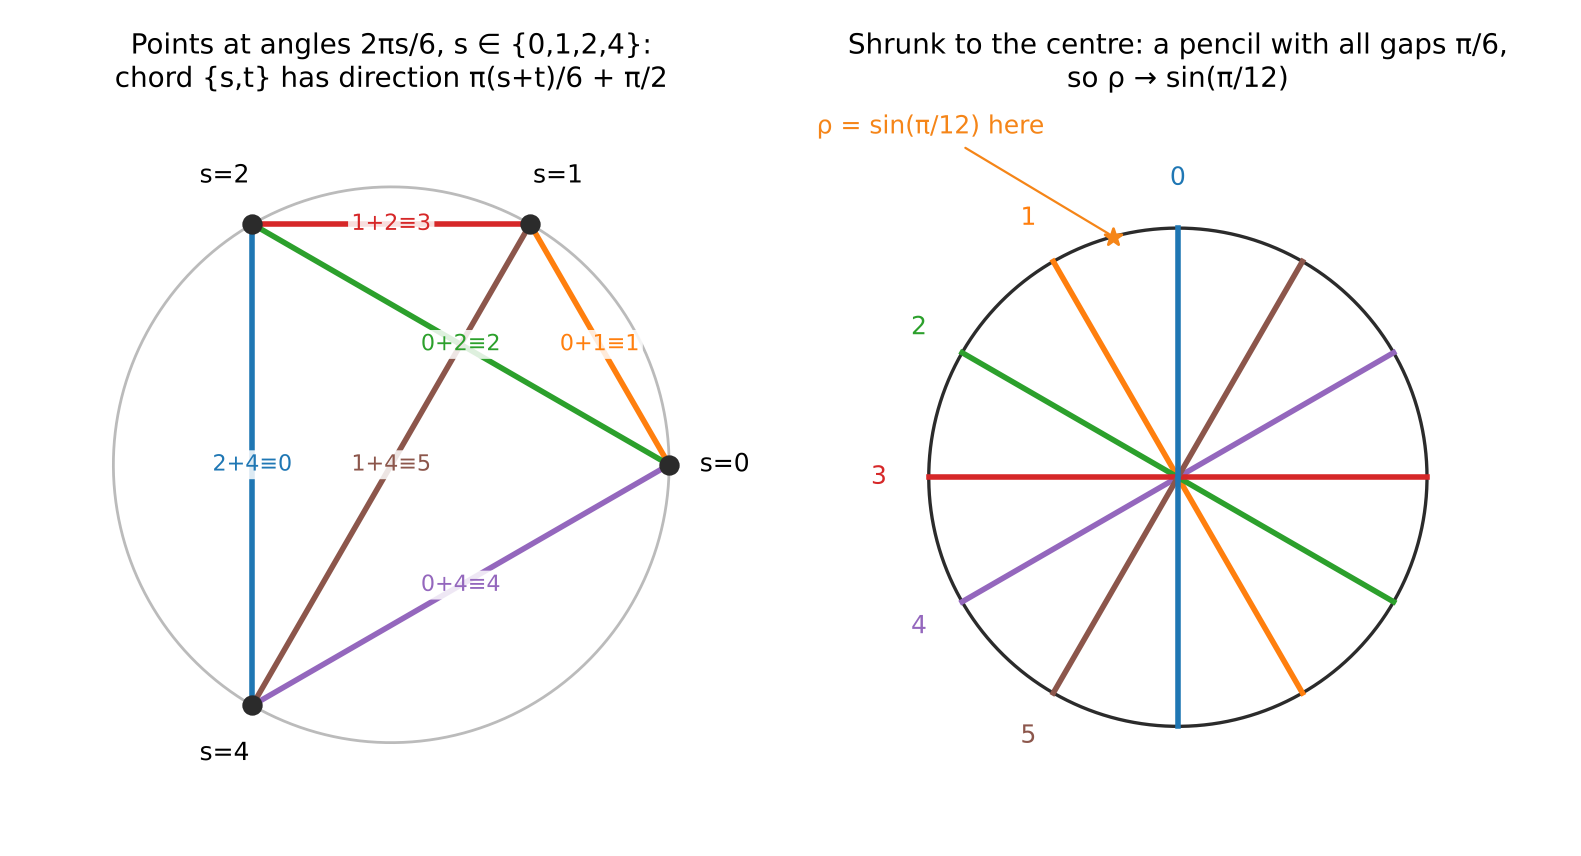
\includegraphics[width=0.85\textwidth]{figures/fig2_sums.png}
\caption{Points at angles $2\pi s/6$, $s\in\{0,1,2,4\}$, on a circle (left). The chord through $s$ and
$t$ has direction $\pi(s+t)/6+\pi/2$ (mod $\pi$: lines are unoriented), and the six pair sums hit every residue mod $6$. Shrunk to the
centre (right), the six lines form a pencil with all gaps $\pi/6$, so $\rho\to\sin(\pi/12)$. This is
the case $d=2$, $N=6$ of Theorem~B.}\label{fig:sums}
\end{figure}

For $d=2$, $p_2(n)$ is Graham and Sloane's $n_\gamma(n)$ \cite{GS}; they proved
$p_2(n)>(5/18)(n-1)^2$, and Jia and Shen \cite{JS} proved $(1/3-o(1))n^2$ for the unrestricted problem,
where a summand may repeat.

\begin{corTwo}
$\sigma_2\ge7/18$, that is, $p_2(n)\ge(7/18-o(1))n^2$; since a restricted cover is also an unrestricted
one, the same bound holds for the unrestricted problem.
\end{corTwo}

The proof is one line: by Theorem~B, $\sigma_2=\sup_np_2(n)/n^2\ge p_2(12)/144\ge56/144$, using the seed
$(12,56)$ from Haanpää's table \cite{Haanpaa} (Appendix~\ref{sec:B-sigma2}, where every residue mod $56$ is
listed as a sum). This exceeds both bounds. We found no larger published
asymptotic constant in these papers, in Haanpää's paper or in Bajnok's problem book \cite{Bajnok}, whose
section on restricted sums with a fixed number of terms lists no results; a check by a specialist in
additive bases is still advisable.

\section{Clusters and small \texorpdfstring{$n$}{n}}\label{sec:small}

\begin{propThree}
If $k$ hyperplanes lie within distance $r$ of the centre and have covering radius $\eps<1-r$, then
$k\cdot[\arccos(r-\eps)-\arccos(r+\eps)]\ge\pi$.
\end{propThree}

\begin{proof}
The slab at offset $|m|\le r$ meets the boundary sphere in a spherical segment of width
$\arccos(|m|-\eps)-\arccos(|m|+\eps)$, which increases with $|m|$. In the plane these are two arcs, so
$2k\cdot w\ge2\pi$ directly; for $d\ge3$ we use Corollary~1.15 of Glazyrin, Karasev and Polyanskii
\cite{GKP}: if $\Sph^{d-1}$ is covered by spherical segments, then the sum of their widths is at least
$\pi$. There a spherical segment of width $2\delta$ is the closed $\delta$-neighbourhood, in the
geodesic metric, of $\Sph^{d-1}\cap H$ for an affine hyperplane $H$. Our slab meets $\Sph^{d-1}$ in
exactly such a set: the points at angle between $\arccos(|m|+\eps)$ and $\arccos(|m|-\eps)$ from $\pm u$,
which is the geodesic neighbourhood of the level set at the middle angle. It is a proper segment because
$\eps<1-r$ keeps $|m|\pm\eps$ inside $(-1,1)$.
\end{proof}

Configurations whose hyperplanes all pass within $o(1)$ of the centre, such as the clusters of
Theorem~B, therefore cost at least $(\pi/2)\cdot d!$, and $\pi$ in the plane. Since
the clusters of Theorem~B achieve $\pi/(2\sigma_d)$, any improvement of this bound for near-flat
clusters would give $\sigma_d<1/d!$; the converse is not known.

\paragraph{Small $n$ in the plane.} Figure~\ref{fig:constants} compares the best known values with
the asymptotic constants.
\begin{itemize}
\item \textbf{$n=3$.} The inscribed equilateral triangle gives $\lambda_2(3)\le1/2$: its sides are
$\ip{x}{a_i}=-1/2$ with $\sum a_i=0$, so every $x\in D$ has some $\ip{x}{a_i}\in[-1,0]$
(Appendix~\ref{sec:B-triangle}).
\item \textbf{$n=4$.} The square $(\pm a,\pm a)$ spans $x=\pm a$, $y=\pm a$ and $y=\pm x$. By the
symmetries of the square take $0\le y\le x$. A point farther than $a$ from all six lines has $x>2a$,
$y>2a$ and $x-y>\sqrt2\,a$, so $x^2+y^2>(4+(2+\sqrt2)^2)a^2=1$. Hence $\rho\le a$, with equality at
$(0,1)$. Shrinking central clusters have $\rho\to$ at least $\sin(\pi/12)\approx0.2588$ by
Proposition~3 ($k=6$), so the square beats them.
\item \textbf{$n=6$.} Take the regular hexagon of radius $r=1/\sqrt{14+4\sqrt3}$ centred at $0$. Its 15
lines are, in directions $0^\circ,60^\circ,120^\circ$, a long diagonal and two sides at offsets
$\pm r\sqrt3/2$, and in directions $30^\circ,90^\circ,150^\circ$, two short diagonals at offsets
$\pm r/2$. The dihedral group of order 12 permutes them, so take $0\le\arg z\le30^\circ$ (Figure~\ref{fig:hexsector}). Distance
$>r/2$ from $y=0$ and from the side $y=r\sqrt3/2$ forces $y>(1+\sqrt3)r/2$; in this sector
$x/2-(\sqrt3/2)y\ge0$, so distance $>r/2$ from the short diagonal $x/2-(\sqrt3/2)y=r/2$ forces
$x>2r+\sqrt3y>(7+\sqrt3)r/2$. Then $|z|^2>r^2(14+4\sqrt3)=1$. Hence $\rho\le r/2$, with equality at
$(0,1)$. Here Proposition~3 gives only $\sin(\pi/30)$ for clusters, hence the certificate below.
\item \textbf{Certified $\gamma_6$.} A cluster ties the hexagon only if $\gamma_6\le12.5495^\circ$.
Table~\ref{tab:gamma} lists the certified bounds. A box branch-and-bound in exact integer arithmetic
gives the lower bounds, and explicit configurations evaluated in interval arithmetic give the upper
bounds. The search prunes using the fact that $\binom n2$ directions with all gaps below $\theta$
leave only $\binom n2\theta-\pi$ of slack.
\item \textbf{Polygons.} A regular $m$-gon of radius $r$ centred at $0$ spans only $m$ line directions mod
$\pi$, equally spaced (the chord through vertices $s$ and $t$ has direction $\pi(s+t)/m+\pi/2$, and the
pairs $(0,c)$ and $(1,m-1)$ give every residue $c$ of $s+t$), and all its lines pass within $r$ of the
centre; so $\rho\ge\sin(\pi/(2m))-r$, by the argument for clusters above. For $r\le1/m$ this gives
$m^2\rho\ge m(m\sin(\pi/(2m))-1)\to\infty$: small regular polygons waste most of their $\binom m2$
lines on repeated directions. We have no bound for larger radii; for $m=4$ and $m=6$, Theorem~D shows that
suitably sized regular polygons beat every shrinking cluster.
\end{itemize}

\begin{table}[ht]
\centering
\caption{Certified bounds on $\gamma_5$ and $\gamma_6$.}\label{tab:gamma}
\small
\begin{tabular}{lp{3.1cm}lp{5.0cm}}
\toprule
Quantity & Lower bound & Upper bound & Runs of the lower-bound computation\\
\midrule
$\gamma_6$ & $12.6792^\circ$ & $12.6800^\circ$ & two, identical (45,959,045 nodes, none unresolved)\\
$\gamma_5$ & $19.6265^\circ$ & $19.6270^\circ$ & two, identical (1,086,476 nodes, none unresolved)\\
\bottomrule
\end{tabular}
\end{table}

\begin{figure}[t]
\centering
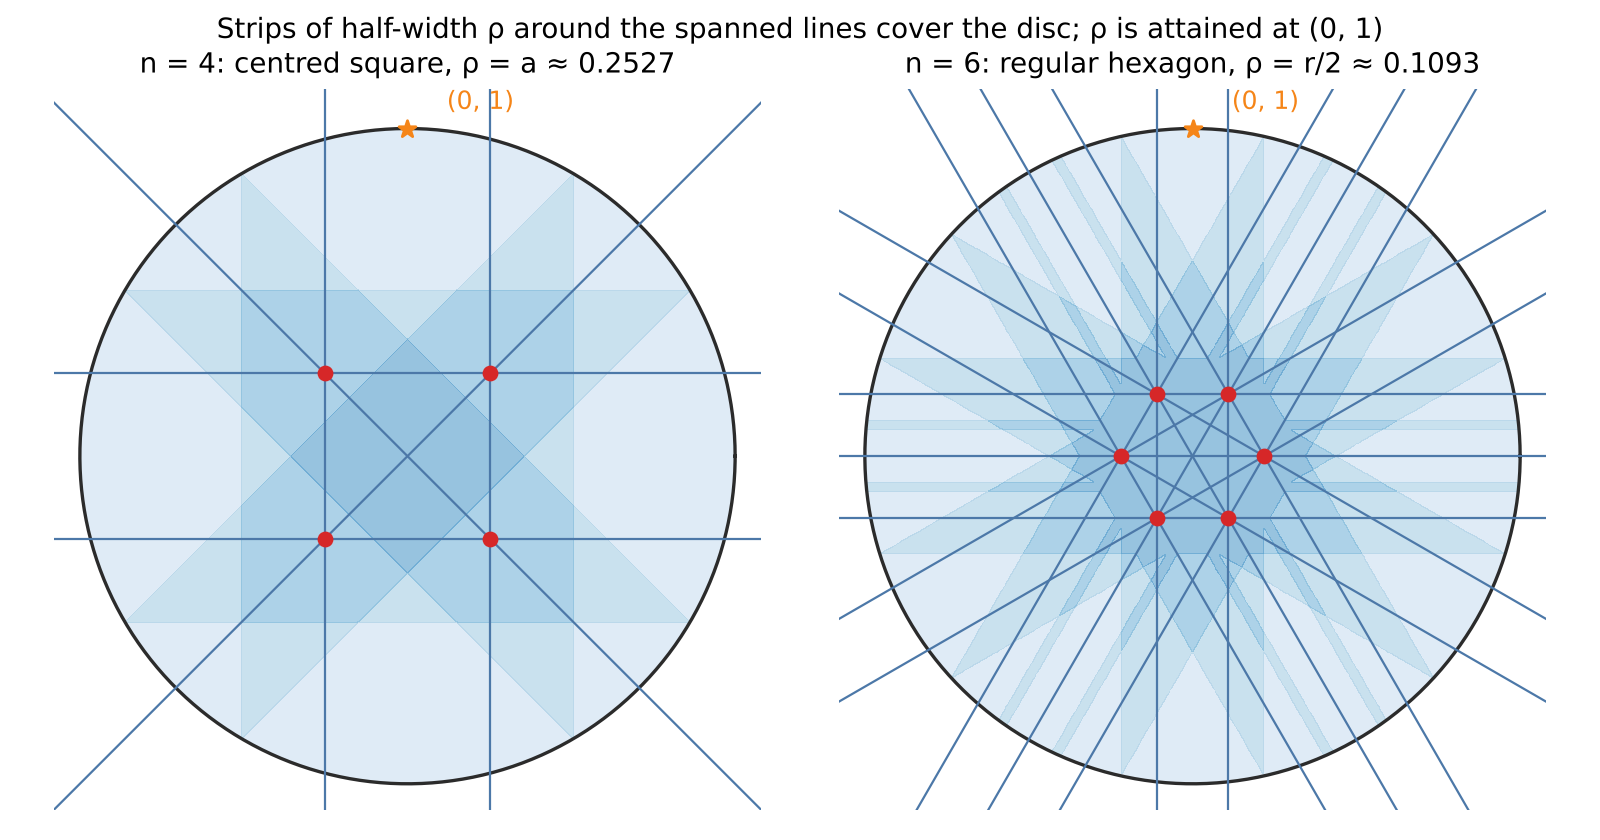
\includegraphics[width=0.8\textwidth]{figures/fig1_square_hexagon.png}
\caption{The centred square ($n=4$) and the regular hexagon ($n=6$) of Theorem~D, with their spanned
lines and the strips of half-width $\rho$ around them (darker where strips overlap). In both, $\rho$ is
attained at the boundary point $(0,1)$.}\label{fig:square}
\end{figure}

\begin{figure}[t]
\centering
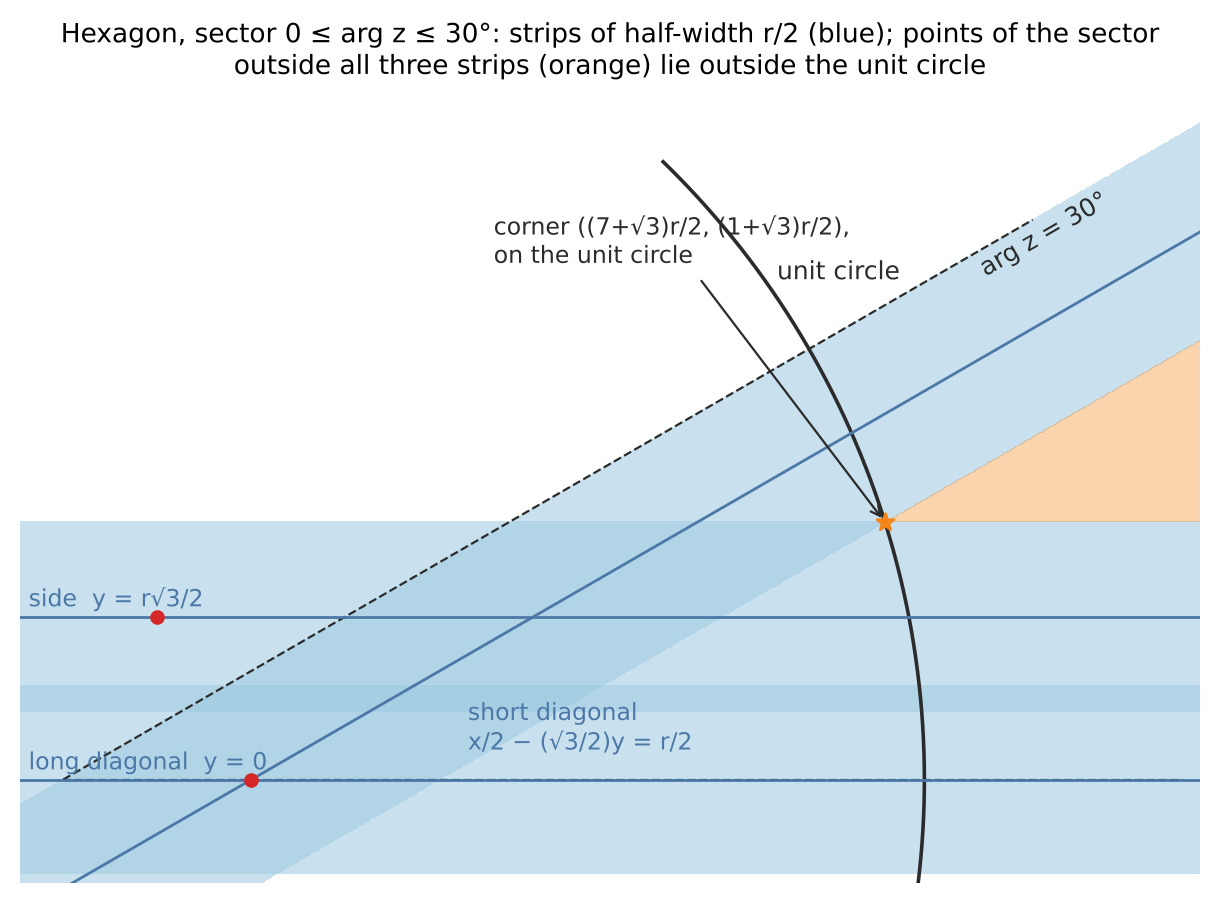
\includegraphics[width=0.62\textwidth]{figures/fig4_hexagon_sector.png}
\caption{The sector argument for the hexagon in Theorem~D. In the sector $0\le\arg z\le30^\circ$, a point at
distance more than $r/2$ from the long diagonal $y=0$, the side $y=r\sqrt3/2$ and the short diagonal
$x/2-(\sqrt3/2)y=r/2$ lies in the orange region, whose corner $\bigl((7+\sqrt3)r/2,(1+\sqrt3)r/2\bigr)$ is on
the unit circle; so no point of the disc is that far from all $15$ lines.}\label{fig:hexsector}
\end{figure}

\begin{center}
\small
\begin{tabular}{p{3.6cm}cccccccc}
\toprule
$n$ & 5 & 6 & 7 & 8 & 9 & 10 & 11 & 12\\
\midrule
$n^2\sin(\gamma_n/2)$, best configuration found (floating point; for $n\ge8$ the searches did not converge) & 4.261 & 3.975 & 4.051 & 4.044 & 4.045 & 4.185 & 4.095 & 4.274\\
\bottomrule
\end{tabular}
\end{center}

\begin{figure}[t]
\centering
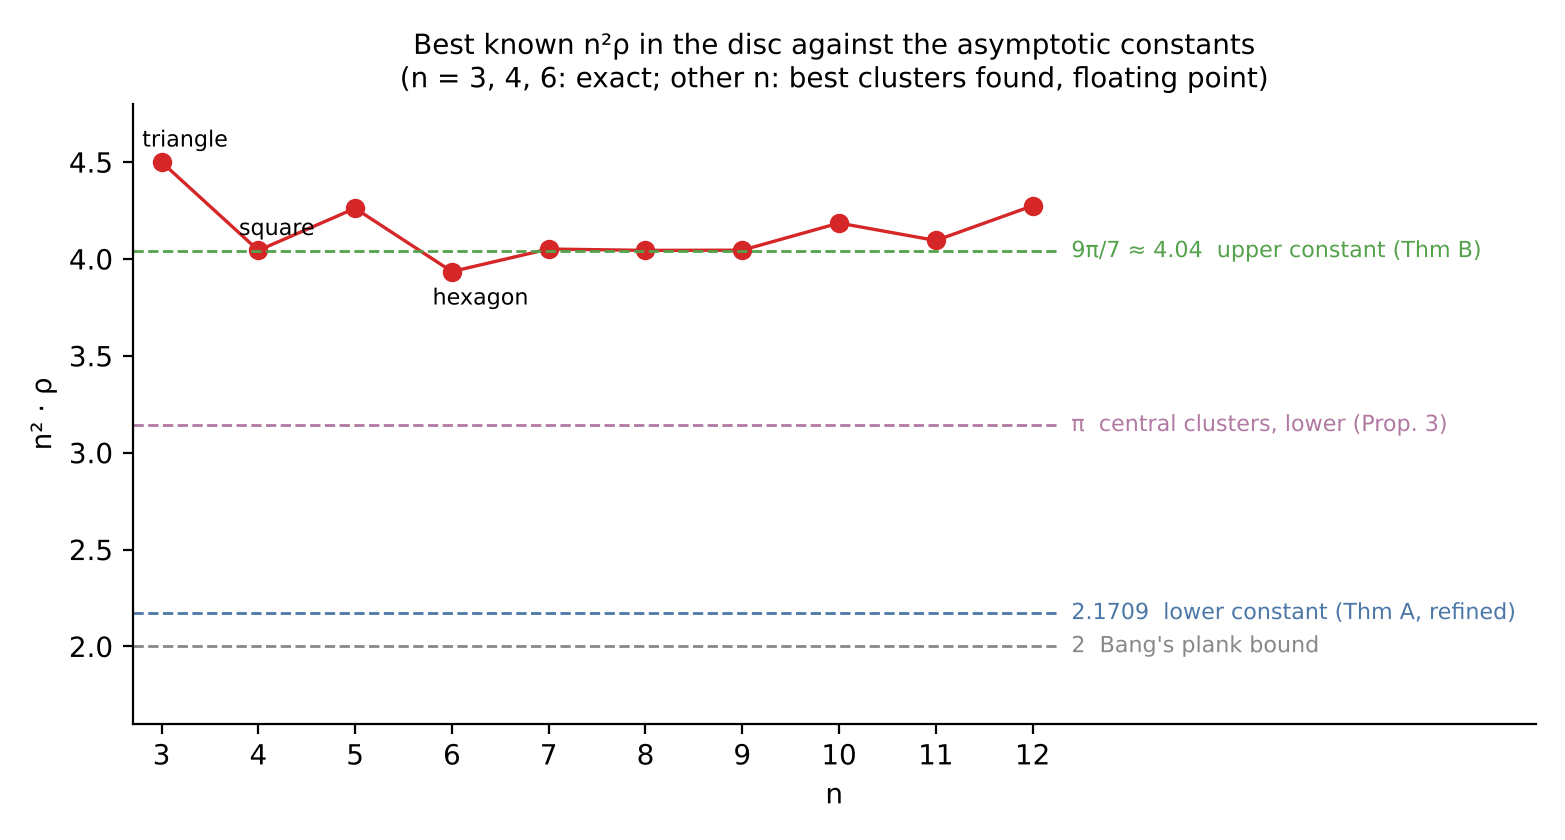
\includegraphics[width=0.8\textwidth]{figures/fig3_constants.png}
\caption{Best known $n^2\rho$ for $n=3,\dots,12$ (triangle, square and hexagon exact; the other values
are the best clusters found, floating point) against the asymptotic constants: Bang's $2$, the lower
constant $6864/3161\approx2.1715$ of Appendix~\ref{sec:A-sharp}, the cluster bound $\pi$ of Proposition~3, and the upper constant
$9\pi/7$ of Theorem~B.}\label{fig:constants}
\end{figure}

\section{Random points}\label{sec:random}

\begin{proof}[Proof sketch of Theorem E (full proofs in Appendix~\ref{app:C})]
Poissonise with mean $(1\mp\theta_0)n$ and discretise $\Omega$ into tiny cells: then ``$x$ is uncovered''
becomes ``no $d$-set of cells from a fixed family is fully occupied'', an event on independent occupancy
indicators, and the mean number $\mu_x$ of spanned hyperplanes within $\eps$ of $x$ is of order $n^d\eps$. The
geometric input is that the hyperplane through $d$ uniform points of $\Omega$ passes within $t$ of a given
point $z$ with probability $h_\Omega(z)t+o(t)$, uniformly in $z$: given the first $d-1$ points, the last must make the
hyperplane's angle in the pencil through their $(d-2)$-flat fall in an interval of length about $t$
divided by the distance to that flat.
\begin{itemize}
\item \textbf{Upper bound.} Janson's inequality \cite{Janson} gives $\Pr(x\text{ uncovered})\le e^{-\mu_x+\Delta_J}$,
where $\Delta_J=O((\log n)^3/n)$ because two $d$-sets sharing cells rarely both pass near $x$. For
$\eps=C\log n/n^d$ with $C>c_\Omega$, $\mu_x>(d^2+\eta)\log n$ for every $x$, and a union bound over a net of
about $n^{d^2}$ points finishes the proof.
\item \textbf{Lower bound.} Harris's inequality \cite{Harris} gives $\Pr(x\text{ uncovered})\ge(1-o(1))e^{-\mu_x}$. A
hyperplane passes within $t$ of two points at distance $r$ with probability $O(t^2/r)$, so Janson makes test
points at distance $\ge(\log n)^3/n^d$ almost independent, and a second moment over about $n^{d^2}$ test points
placed near a minimiser of $h_\Omega$ finds an uncovered one when $\mu_x<(d^2-\eta)\log n$, i.e.\ for
$\eps=c\log n/n^d$ with any $c<c_\Omega$ (Appendix~\ref{sec:C-all-d}).\qedhere
\end{itemize}
\end{proof}

In floating-point experiments in the disc (medians over $n=8,\dots,40$), $n^2\rho/\log n$ is about $10$ to $12$,
against the limit $9\pi^2/8\approx11.10$, which is set by the boundary of the disc, where $h_\Omega$ is smallest.

\section{Variants}\label{sec:variants}

\paragraph{Great hyperspheres.} For $n>d$ points on $\Sph^d$ and the great hyperspheres through $d$ of
them, the infimum of the angular covering radius lies between $\pi/(2K)$ and $\pi/(2p_d(n))$: project
the construction of Theorem~B gnomonically. The bounds coincide when $p_d(n)=\binom nd$, for example for
$n=d+1$ (take $\Z_{d+1}$) and for $(n,d)=(4,2),(6,3)$ (for the latter, the $20$ three-sums of $\{1,4,10,17,18,19\}\subset\Z_{20}$ are distinct); so the infimum is $\pi/(2(d+1))$ for $n=d+1$
(Appendix~\ref{sec:D-spheres}).

\paragraph{Points anywhere.} Let $\mu_d(n)$ be the infimum of $\rho$ when the $n$ points may lie
anywhere in $\R^d$. Then $1/\binom nd\le\mu_d(n)\le1/N_d(n)$, where $N_d(n)$ is the longest run of
consecutive integers among the sums of $d$ distinct elements of an $n$-set of positive integers. The
upper bound sends the points $(Xt,\dots,Xt^{d-1},\alpha/t+\beta)$, $t=1/u$, to infinity: the hyperplane
through $d$ of them tends to a horizontal one at height $\alpha\sum u+\beta$, because the interpolant of
$1/t$ at $d$ nodes $t_i$ takes the value $\sum1/t_i$ at $0$. So $\mu_d(d+1)=1/(d+1)$, and digit blocks
give $N_d(dq)\ge q^d$, so $d!\le\liminf n^d\mu_d(n)\le\limsup n^d\mu_d(n)\le d^d$. In the plane
$N_2(n)\ge\lfloor n^2/4\rfloor$, $\mu_2(3)=1/3$ and $\mu_2(4)=1/6$ (Lemma~\ref{D:N2}).

\paragraph{Flats through $j+1$ points.} For $1\le j\le d-1$, let $\lambda_d^{(j)}(n)$ be the analogue of
$\lambda_d(n)$ for the $j$-flats spanned by $j+1$ of the $n$ points (so $j=d-1$ is the main problem).
Then $\lambda_d^{(j)}(n)=\Theta(n^{-(j+1)/(d-j)})$. For the lower bound, if the $\rho$-neighbourhoods of
$K$ $j$-flats cover $\ball^d$ then $K\rho^{d-j}\ge c(d,j)$, with $c(d,1)=1$ and
$c(d,j)=\Gamma(j/2)\Gamma((d-j)/2+1)/\Gamma(d/2)$ for $j\ge2$: the density $(1-|x|^2)^{-a}$ ($a=\frac12$
for lines, $a\uparrow1$ otherwise) has its integral over every $j$-flat bounded by the value on a
central one. For lines the density $(1-|x|^2)^{-1/2}$ integrates to exactly $\pi$ along every line,
which gives $k\rho^{d-1}\ge1$; this is the ellipsoid case of Bezdek and Litvak's theorem on covering
convex bodies by cylinders \cite{BL}, proved there with the same density (for $d=2$ it is Bang's bound
for the disc). For the upper bound, put $j+1$ groups of points at moment-curve positions in
$\R^{j-1}\times\{0\}$, each carrying a grid in the complementary $\R^{d-j+1}$ at its own scale; as the
cluster shrinks, the flat through one point of each group tends to $\R^{j-1}\oplus\R w$, where $w$ is
the sum of the chosen grid vectors, and these sums form a complete digit grid of directions in one chart; $d-j+1$ rotated copies of the
cluster cover all directions. This is
Lemma~2. It gives
$\limsup n^{(j+1)/(d-j)}\lambda\le\sqrt{d-j}\,\bigl((d-j+1)(j+1)\bigr)^{(j+1)/(d-j)}$; for lines in
$\ball^3$, $\sqrt2\le\liminf n\lambda\le\limsup n\lambda\le6\sqrt2$ (Appendix~\ref{sec:D-flats}).

\section{General convex bodies}\label{sec:convex}

Let $\Omega$ be a convex body, with minimal width $w(\Omega)$, circumradius $R(\Omega)$, volume $|\Omega|$
and diameter $\operatorname{diam}\Omega$, and define $\lambda_d(n;\Omega)$, $\mu_d(n;\Omega)$ and
$\rho_\Omega$ as before, with points in $\Omega$ (or anywhere) and slabs covering $\Omega$. The order of every
covering radius in this paper extends; the sharp results do not.

\begin{center}
\small
\begin{tabular}{p{3.4cm}p{5.2cm}p{5.6cm}}
\toprule
Result & Unit ball & Convex body $\Omega$\\
\midrule
Order of $\lambda_d(n)$ & $\ell_d\le\liminf n^d\lambda_d(n)$ (Corollary~C), $\limsup\le\pi/(2\sigma_d)$ &
$d!\,w(\Omega)/2\le\liminf n^d\lambda_d(n;\Omega)$, $\limsup\le\pi R(\Omega)/(2\sigma_d)$\\
Points anywhere, $n=d+1$ & $\mu_d(d+1)=1/(d+1)$ & $\mu_d(d+1;\Omega)=w(\Omega)/(2(d+1))$\\
Random points & $n^d\rho/\log n\to c_{\ball^d}$; $c_{\ball^2}=9\pi^2/8$ &
$n^d\rho_\Omega/\log n\to c_\Omega$ (Theorem~E)\\
Strict gain over Bang (Theorem~A, Corollary~1$'$) & yes & open\\
Small $n$, $\gamma_n$, $6864/3161$, the cluster limit $\sin(G/2)$ & Theorem~D, Table~\ref{tab:gamma} & not treated\\
\bottomrule
\end{tabular}
\end{center}

\paragraph{Hyperplanes.} Bang's plank theorem (Verreault's survey \cite{Verreault}, Theorem~2.2) gives
$\mu_d(n;\Omega)\ge w(\Omega)/(2\binom nd)$. The clusters of Theorem~B, scaled into $\Omega$ around interior
points (taking the infimum over them), give $\lambda_d(n;\Omega)\le R(\Omega)\sin(\pi/(2p_d(n)))$; and the
points-anywhere construction, with horizontal hyperplanes in a direction of minimal width, gives
$\mu_d(n;\Omega)\le w(\Omega)/(2N_d(n))$. This gives the first two rows (Appendix~\ref{sec:D-convex}).

\paragraph{Random points.} Theorem~E is proved for every convex body in every dimension directly
(Appendix~\ref{app:C}), with the exact limit constant $c_\Omega$; Remark~\ref{rem:C-plane} gives its planar formula.

\section{Open problems}\label{sec:open}

\begin{enumerate}
\item Does $\lim n^2\lambda_2(n)$ exist, and what is it? The liminf and limsup lie in
$[2.1714,\,9\pi/7\approx4.04]$; floating-point searches for $n\le12$ suggest about $4$.
\item Are shrinking clusters optimal for odd $n$, and asymptotically? For $n=5$, can any finite
configuration beat $\sin(\gamma_5/2)$?
\item Determine $\sigma_d$. Known: $7/18\le\sigma_2\le1/2$ and $19/200\le\sigma_3\le1/6$; the upper
bounds are only the count $p_d(n)\le\binom nd$ (for $d=2$, Haanpää's table gives $p_2(n)<\binom n2$ for $5\le n\le14$,
but no constant below $1/2$ is known).
\item Is $\lambda_2(3)=1/2$? Is $\lambda_2(4)=1/\sqrt{10+4\sqrt2}$?
\item Flats: $\lambda_d^{(j)}(n)=\Theta(n^{-(j+1)/(d-j)})$ (\S\ref{sec:variants}), but the constants are
far apart (for lines in $\ball^3$, between $\sqrt2$ and $6\sqrt2$). Is there a strict bound beyond
$c(d,j)$ for spanned flats, as Theorem~A gives for hyperplanes, and do better direction designs lower
the upper constants?
\item Does the gain over Bang survive in high dimension, that is, is $\inf_d(L_d/d!-1)>0$? Theorem~A
gives only $L_d/d!-1\ge0.08/\sqrt{d-2}$; the loss is built into the method: under the measure of the
proof, a slab of half-width $\eps$ through the centre with normal perpendicular to $v$ carries
$\Phi$-mass about $C_d(m_0^2+\frac12)\eps$, where $C_d\approx\sqrt{\pi d/2}$, against
$(m_0^2+\frac12)\eps$ in the flat case. A different measure or test function would be needed.
\item For a convex body $\Omega$, how does $n^d\lambda_d(n;\Omega)$ depend on the shape of $\Omega$? The bounds
$d!\,w(\Omega)/2$ and $\pi R(\Omega)/(2\sigma_d)$ are far apart for thin bodies, where a pencil of hyperplanes
through a common $(d-2)$-flat is wasteful; points placed anywhere do reach the width scale $w(\Omega)$.
\end{enumerate}

\section*{Computations and full proofs}

The only computer-assisted results are the bounds of Table~\ref{tab:gamma}: exact integer
branch-and-bound for the lower bounds and interval arithmetic for the upper bounds. The comparison of
the hexagon with shrinking clusters in Theorem~D rests on them. The repository accompanying this paper,
\url{https://github.com/michael-werman/planks}, holds their code, input data, command, runtime and output (folder
\texttt{certificates/\allowbreak gamma6\_\allowbreak gamma5}). Everything else is proved by hand; the finite examples are given
with one representation of every residue (Lemma~\ref{lem:B-seed} and Section~\ref{sec:B-examples}). The
repository also holds independent exact re-checks: the hexagon value ($\rho^2$ exact in $\Q(\sqrt3)$), the
seeds and two blown-up instances of the additive bases, the seed behind
$\sigma_2\ge7/18$, and the algebra of Appendix~\ref{app:A}. Appendices~\ref{app:A}--\ref{app:D} give
complete proofs of the results sketched in the main text.

\begin{thebibliography}{99}
\bibitem{Bajnok} B.~Bajnok, Additive Combinatorics: A Menu of Research Problems, arXiv:1705.07444 (2017).
\bibitem{Bang} T.~Bang, A solution of the ``plank problem'', Proc. Amer. Math. Soc. 2 (1951), 990--993.
\bibitem{BL} K.~Bezdek and A.~E. Litvak, Covering convex bodies by cylinders and lattice points by
flats, J. Geom. Anal. 19 (2009), 233--243.
\bibitem{FM} P.~Frankl and H.~Maehara, Projecting a finite point-set into a hyperplane, Ryukyu Math. J.
8 (1995), 27--35.
\bibitem{Gardner} R.~J. Gardner, Relative width measures and the plank problem, Pacific J. Math. 135
(1988), 299--312.
\bibitem{GKP} A.~Glazyrin, R.~Karasev and A.~Polyanskii, Covering by planks and avoiding zeros of
polynomials, Int. Math. Res. Not. IMRN 2023, no.~13, 11684--11700.
\bibitem{GS} R.~L. Graham and N.~J.~A. Sloane, On additive bases and harmonious graphs, SIAM J.
Algebraic Discrete Methods 1 (1980), 382--404.
\bibitem{Haanpaa} H.~Haanpää, Minimum sum and difference covers of abelian groups, J. Integer Seq. 7
(2004), Art.~04.2.6.
\bibitem{Harris} T.~E. Harris, A lower bound for the critical probability in a certain percolation
process, Proc. Cambridge Philos. Soc. 56 (1960), 13--20.
\bibitem{Janson} S.~Janson, Poisson approximation for large deviations, Random Structures Algorithms 1
(1990), 221--229.
\bibitem{JS} X.~Jia and J.~Shen, Extremal bases for finite cyclic groups, SIAM J. Discrete Math. 31
(2017), 796--804.
\bibitem{JP} Z.~Jiang and A.~Polyanskii, Proof of László Fejes Tóth's zone conjecture, Geom. Funct.
Anal. 27 (2017), 1367--1377.
\bibitem{Verreault} W.~Verreault, Plank theorems and their applications: a survey, Bull. LMS 58 (2026),
e70230; arXiv:2203.05540.
\bibitem{ZhaoNotes} Y.~Zhao, Probabilistic Methods in Combinatorics, lecture notes, MIT 18.226 (version of June 18,
2024), \url{https://yufeizhao.com/pm/probmethod_notes.pdf}.
\bibitem{Zhao} Y.~Zhao, Exploring a planet, revisited, Amer. Math. Monthly 129 (2022), 678--680.
\end{thebibliography}

\appendix
\IfFileExists{appendix_A.tex}{\section{Proofs for the lower bound (Theorem A, Corollary 1$'$)}
\label{app:A}

% Local notation for this appendix.
\newcommand{\Abb}{\bar\beta}
\newcommand{\AH}{\mathcal{H}}
\newcommand{\AI}{\mathcal{I}}
\newcommand{\Aone}{\mathbf{1}}
\newcommand{\Adep}{\#\mathrm{dep}}

% ======================================================================
\subsection{Spanned hyperplanes never attain Bang's bound, in every dimension}
\label{sec:A-strict}

This subsection proves Corollary~1$'$ of the main text, $\lambda_d(n) > 1/\binom nd$ for every
$d \ge 2$ and $n > d$. The proof uses only Lemma~1.

\subsubsection*{Definitions}

\begin{itemize}
  \item $\ball^d$ is the closed unit ball. For $P \subset \ball^d$ with $n$ points, $\AH_P$ is the
    set of hyperplanes spanned by affinely independent $d$-subsets of $P$.
    $\rho(P) = \max_{x \in \ball^d} \min_{H \in \AH_P} \dist(x, H)$, and $\rho = \infty$ if
    $\AH_P = \emptyset$. $\lambda_d(n) = \inf\{\rho(P) : P \subset \ball^d,\ |P| = n\}$.
    $K = \binom{n}{d}$.
  \item For a finite list of hyperplanes $\{\ip{x}{u_j} = m_j\}$ ($|u_j| = 1$), its
    \emph{covering radius} is
    \begin{equation*}
      \max_{x \in \ball^d} \min_j \dist(x, H_j).
    \end{equation*}
    It depends only on the set of hyperplanes.
\end{itemize}

By Lemma~1 (Section~\ref{sec:lower}), if the closed $\eps$-slabs around $k$ hyperplanes
$\{\ip{x}{u_j} = m_j\}$ cover $\ball^d$, then $\eps \max_{|v|=1}\sum_j|\ip{u_j}{v}| \ge 1$. In particular a covering list of $k$ hyperplanes has covering radius at least $1/k$, so
$\lambda_d(n) \ge 1/K$.

\subsubsection*{Statement}

\begin{proposition}\label{prop:A-strict}
For $d \ge 2$ and $n \ge d + 1$, $\lambda_d(n) > 1/\binom{n}{d}$. (For $n = d$ there is at most one
hyperplane, and $\lambda_d(d) = 1 = 1/K$, attained by $d$ independent points on a hyperplane
through the centre.)
\end{proposition}

\begin{proof}
Suppose $\lambda_d(n) = 1/K$, and take labelled $n$-point sets $P_k$ with $\rho(P_k) \to 1/K$.
Pass to a subsequence along which:
\begin{enumerate}[label=(\roman*)]
  \item the family $\AI$ of affinely independent $d$-subsets (by labels) is the same for all $k$;
  \item each labelled point converges, $p_i^{(k)} \to p_i \in \ball^d$;
  \item for each $F \in \AI$, the hyperplane of $F$, written
    $\{\ip{x}{u_F^{(k)}} = m_F^{(k)}\}$ with $|u| = 1$ and $|m| \le 1$, has $u_F^{(k)} \to u_F$
    and $m_F^{(k)} \to m_F$.
\end{enumerate}
This is possible by compactness: (i) has finitely many possibilities, and $|m| \le 1$ because the
hyperplane meets $\ball^d$. The limit hyperplane $H_F = \{\ip{x}{u_F} = m_F\}$ contains $p_i$ for
every $i \in F$, by continuity of $\ip{p_i^{(k)}}{u_F^{(k)}} - m_F^{(k)} = 0$.

For $|x| \le 1$ we have $|\dist(x, H) - \dist(x, H')| \le |u - u'| + |m - m'|$. Along the
subsequence $\AH_{P_k} = \{H_F^{(k)} : F \in \AI\}$, and a min over a finite family followed by a
max over $\ball^d$ is $1$-Lipschitz in the sup norm. So the covering radius of the list
$(H_F)_{F \in \AI}$ is the limit of $\rho(P_k)$, namely $1/K$. $\AI \ne \emptyset$, since
otherwise $\rho(P_k) = \infty$. If $|\AI| < K$, Lemma~1 would give covering radius
$\ge 1/|\AI| > 1/K$ for each $P_k$ (a bound independent of $k$), contradicting
$\rho(P_k) \to 1/K$. So $|\AI| = K$: every $d$-subset is independent.

Apply Lemma~1 to the list $(H_F)$ with $\eps = 1/K$. Then
$\max_v \sum_F |\ip{u_F}{v}| \ge K$. Since each term is at most $1$ and there are $K$ terms, some
unit $v$ has $|\ip{u_F}{v}| = 1$ for all $F$. So every $H_F$ is $\{\ip{x}{v} = b_F\}$ for some
$b_F$. Their $1/K$-slabs cover $\ball^d$, in particular the diameter $\{tv : |t| \le 1\}$. So the
$K$ intervals $[b_F - 1/K,\, b_F + 1/K]$ cover $[-1, 1]$, whose length $2$ equals their total
length. Hence any two of them meet in at most one point, and the $b_F$ are pairwise distinct.

Since $n \ge d + 1$ and $d \ge 2$, the $d$-sets $F = \{1, \dots, d\}$ and
$F' = \{2, \dots, d+1\}$ are distinct and share the point $p_2$. Both $H_F$ and $H_{F'}$ contain
$p_2$, so $b_F = \ip{p_2}{v} = b_{F'}$. This is a contradiction.
\end{proof}

\begin{remark}
The limit points $p_i$ may coincide, and the limit hyperplanes need not be spanned by the limit
points. The proof uses only that $H_F$ contains $p_i$ for $i \in F$.
\end{remark}

% ======================================================================
\subsection{\texorpdfstring{Theorem~A in every dimension $d \ge 2$: one statement, one proof}%
{Theorem A in every dimension d >= 2: one statement, one proof}}
\label{sec:A-unified}

This proves the $d = 2$, $d = 3$ and $d \ge 4$ cases of Theorem~A together.

\subsubsection*{Definitions}

\begin{itemize}
  \item $\ball^d$ is the closed unit ball and $\Sph^{d-1}$ its boundary. $P \subset \ball^d$ has
    $n$ points, and $K = \binom{n}{d}$.
  \item $\AH'$ is the set of distinct hyperplanes spanned by affinely independent $d$-subsets of
    $P$, and $K' = |\AH'|$. For $H \in \AH'$, $N_H \ge 1$ is the number of independent $d$-subsets
    lying in $H$.
  \item $\eps = \rho(P) = \max_{x \in \ball^d} \min_{H \in \AH'} \dist(x, H)$, and $S_H$ is the
    closed $\eps$-slab around $H$. If $P$ has no $d$ affinely independent points,
    $\rho = \infty$ and there is nothing to prove.
  \item $\lambda_d(n) = \inf\{\rho(P) : P \subset \ball^d,\ |P| = n\}$.
  \item $A_d = (3d - 1)/(d - 1)$, so $A_2 = 5$ and $A_3 = 4$.
  \item For $d \le 3$ put $\Lambda_d(m) = A_d$. For $d \ge 4$ put $\Abb_d = 2/(d-1)$,
    $C_d = \sqrt{\pi}\, \Gamma((d-1)/2) / \Gamma((d-2)/2)$ (so $C_4 = \pi/2$, $C_5 = 2$,
    $C_{d+2} = C_d (d-1)/(d-2)$), and
    \begin{equation*}
      \Lambda_d(m) = A_d + (1+|m|)^2(C_d - 1)
        + 4(1+|m|)(1 - \Abb_d).
    \end{equation*}
  \item $q_d = \min_{|m| \le 1} (1/3 + m^2)/\Lambda_d(m)$. So $q_2 = 1/15$ and $q_3 = 1/12$.
\end{itemize}

\subsubsection*{Theorem~A}

\begingroup\itshape\sloppy
For every $d \ge 2$ and $n \ge d$, every $n$-point set $P \subset \ball^d$ with $\rho = \rho(P)$
satisfies
\begin{equation*}
  \binom{n}{d} \rho \ge \frac{1 + q_d}{1 + 2\rho/A_d}.
\end{equation*}
(If $P$ has no $d$ affinely independent points, $\rho = \infty$ and the bound is trivial.) Hence
$\liminf_n n^d \lambda_d(n) \ge L_d := d!\,(1 + q_d)$.
\begin{itemize}
  \item For $d = 2$ the bound reads $\binom{n}{2}\rho \ge 16/(15 + 6\rho)$, and $L_2 = 32/15$.
  \item For $d = 3$ it reads $\binom{n}{3}\rho \ge 13/(12 + 6\rho)$, and $L_3 = 13/2$.
  \item For $d \ge 4$, $q_d \ge 0.08/\sqrt{d-2}$; also $q_4 \ge 0.0588$ and $q_5 \ge 0.0496$, so
    $L_4 \ge 25.41$ and $L_5 \ge 125.95$ (Section~\ref{sec:A-qd}).
\end{itemize}
\endgroup

\subsubsection*{Proof}

\paragraph{Step 1 (tilt budget).} This is Lemma~1 (Section~\ref{sec:lower}). Here $\eps = \rho(P) > 0$, since finitely many hyperplanes cannot cover $\ball^d$, and the closed
$\eps$-slabs around the $K'$ hyperplanes of $\AH'$ cover $\ball^d$, since the maximum defining
$\rho(P)$ is attained (a maximum over the compact $\ball^d$ of a minimum of finitely many continuous
functions). Apply Lemma~1 to $\AH'$ ($k = K'$) with a maximising unit $v$. Orient each normal so that
$\cos\psi_H = \ip{u_H}{v} \ge 0$, with $\psi_H \in [0, \pi/2]$. Write
$H = \{\ip{x}{u_H} = m_H\}$; then $|m_H| \le 1$, since $H$ meets $P \subset \ball^d$. Put
$\kappa_H = 1 - \cos\psi_H \in [0, 1]$. Since $\sum_H \cos\psi_H \ge 1/\eps$:
\begin{itemize}
  \item[(1a)] $\sum_{H \in \AH'} \kappa_H \le K' - 1/\eps \le K - 1/\eps$.
  \item[(1b)] $\sum_{Q \text{ indep}} \kappa_{H(Q)} + \#\{\text{dependent } d\text{-sets}\} \le
    K - 1/\eps$. Indeed,
    $\sum_Q \kappa = \sum_H N_H \kappa_H \le \sum_H \kappa_H + \sum_H (N_H - 1) \le T - 1/\eps$,
    where $T = \sum_H N_H$, and $\#\text{dependent} = K - T$.
\end{itemize}

The \emph{height} is $t(x) = \ip{x}{v}$. Let $m_0$ be the mean height of $P$, so $|m_0| \le 1$.
Put $\Phi(x) = (t(x) - m_0)^2$ and $M_0 = (1 + |m_0|)^2$.

\paragraph{Step 2 (test measures with uniform height).} Each case uses a probability measure
$\sigma$ whose height $t$ is uniform on $[-1, 1]$, so $\int \Phi \, d\sigma = 1/3 + m_0^2$.
\begin{itemize}
  \item $d = 3$: $\sigma$ is uniform on $\Sph^2$. By Archimedes, for every unit $w$,
    $\ip{y}{w}$ is uniform on $[-1, 1]$, and given $\ip{y}{w} = s$ the point is uniform on the
    circle at that level.
  \item $d = 2$: $\sigma$ is the image of the uniform measure on $\Sph^2 \subset \R^3$ under the
    orthogonal projection onto $\R^2 \supset \ball^2$, which is
    $dx / (2\pi\sqrt{1 - |x|^2})$ on $\ball^2$. A slab $\{|\ip{x}{u} - m| \le \eps\}$ of $\R^2$
    pulls back to the slab of $\R^3$ with the same $u$, $m$, $\eps$, and $\Phi$ pulls back to
    the same quadratic in $\ip{y}{v}$. So every computation below for $d = 3$ applies verbatim.
  \item $d \ge 4$: let $\Pi$ be a uniformly random $2$-plane in $v^\perp$ and
    $V = \R v \oplus \Pi$. Let $\sigma_V$ be uniform on $S_V = \Sph^{d-1} \cap V$, and use
    $\sigma_V$ averaged over $\Pi$. For a unit $e \perp v$, $\beta = |P_\Pi e|^2$ has law
    $\mathrm{Beta}(1, (d-3)/2)$, being $(g_1^2 + g_2^2)/(g_1^2 + \dots + g_{d-1}^2)$ for
    independent Gaussians (here $d - 1 \ge 3$). Hence
    $\E\beta = 2/(d-1) = \Abb_d$ and
    $\E\beta^{-1/2} = \frac{d-3}{2}\, B\bigl(\frac12, \frac{d-3}{2}\bigr)
    = \sqrt\pi\,\Gamma(\frac{d-1}2)/\Gamma(\frac{d-2}2) = C_d$.
\end{itemize}
For $d \le 3$ set $V = \R^3$ and $\beta \equiv 1$ below. In every case the covering
$S_V \subset \bigcup_H S_H$, together with the uniform height on $S_V$, gives
\begin{equation}\label{eq:A-unified-2}
  \frac13 + m_0^2 \le \sum_{H \in \AH'} \E \int_{S_H} \Phi \, d\sigma_V. \tag{2}
\end{equation}

\paragraph{Step 3 (one slab, one section).} Fix $H$ with $a = \cos\psi$, $b = \sin\psi$, offset
$m$, and $u = av + be$ ($e \perp v$ a unit vector, if $b > 0$). Then $P_V u = av + b P_\Pi e$, so
$r := |P_V u| = \sqrt{a^2 + \beta b^2} \in [a, 1]$, and $r > 0$ almost surely ($\beta > 0$ a.s.).
Put $\tilde u = P_V u / r$. Then
$\ip{y}{u} = r \ip{y}{\tilde u}$ on $V$, $\ip{v}{\tilde u} = a/r$ and
$1 - a^2/r^2 = \beta b^2/r^2$. By Archimedes in $V$, $\tilde s = \ip{y}{\tilde u}$ is uniform on
$[-1, 1]$, and
\begin{equation*}
  \E[\Phi \mid \tilde s] = \tilde\Gamma(\tilde s)
    = (\tilde s a/r - m_0)^2 + (1 - \tilde s^2)\, \beta b^2/(2r^2).
\end{equation*}
Since $s = r\tilde s$ has density $1/(2r)$ on $(-r, r)$, averaging over $\Pi$ (Tonelli; everything is
nonnegative) gives
\begin{equation*}
  \E \int_{S_H} \Phi \, d\sigma_V = \frac12 \int_{m-\eps}^{m+\eps} \overline G_H(s) \, ds, \qquad
  \overline G_H(s) = \E\bigl[r^{-1} \tilde\Gamma(s/r)\, \Aone\{|s| < r\}\bigr],
\end{equation*}
and $\overline G_H = 0$ for $|s| \ge 1$. For $d \le 3$, $r \equiv 1$ and
$\overline G_H(s) = G_H(s) \cdot \Aone\{|s| < 1\}$, where
\begin{equation*}
  G_H(s) = (sa - m_0)^2 + (1 - s^2)\, b^2/2.
\end{equation*}

\paragraph{Step 4 (averaging costs only tilt).} For $|s| < 1$ we have
$\overline G_H(s) \le G_H(s) + e(\psi_H)$, with $e \equiv 0$ for $d \le 3$, and for $d \ge 4$
\begin{equation*}
  e(\psi) = M_0(R(\psi) - 1) + 2(1 + |m_0|)(1 - \Abb_d)\, b^2, \qquad R(\psi) = \E[1/r].
\end{equation*}

\begin{proof}[Proof ($d \ge 4$)]
On $\{|s| < r\}$ let $\tilde c = sa/r^2$, $T = \tilde\Gamma(s/r)$ and $\omega = a/r \in [0, 1]$, so the integrand
is $r^{-1}T$.
\begin{itemize}
  \item $T \le M_0$: $|\tilde c| = (|s|/r)\omega \le \omega$ and $\beta b^2/r^2 = 1 - \omega^2$, so
    $T \le (\omega + |m_0|)^2 + (1 - \omega^2)/2$, which is non-decreasing in $\omega$ and equals $M_0$ at $\omega = 1$.
  \item $T \le G_H(s) + 2(1 + |m_0|)(1 - r^2)$: $(\tilde c - m_0)^2 - (sa - m_0)^2 = (\tilde c - sa)(\tilde c + sa - 2m_0)$
    with $|\tilde c - sa| = |\tilde c|(1 - r^2) \le 1 - r^2$ and $|\tilde c + sa - 2m_0| \le 2(1 + |m_0|)$; and
    $(1 - s^2/r^2)\beta b^2/(2r^2) \le (1 - s^2)b^2/2$, as $\beta \le r^2 \le 1$.
\end{itemize}
So $r^{-1}T = T + (r^{-1} - 1)T \le Z := G_H(s) + 2(1 + |m_0|)(1 - r^2) + M_0(r^{-1} - 1)$. $Z \ge 0$ for
$|s| \le 1$, so $\overline G_H(s) \le \E Z = G_H(s) + e(\psi)$, using $\E(1 - r^2) = b^2(1 - \Abb_d)$.
\end{proof}

\begin{lemma}[Lemma~R, $d \ge 4$]
$R(\psi) - 1 \le (C_d - 1)\, \kappa$.
\end{lemma}

\begin{proof}
Let $a = \cos\psi < 1$ (for $a = 1$ both sides vanish) and $k = (d-3)/2$, so $\beta$ has density $k(1-x)^{k-1}$.
Substituting $x = (u^2 - a^2)/(1 - a^2)$, i.e.\ $u = r \in (a, 1)$,
\[
  R - 1 = \E\Bigl[\frac{1 - r}{r}\Bigr] = \frac{2k}{(1 - a^2)^k}N(a), \qquad N(a) = \int_a^1(1 - u)(1 - u^2)^{k-1}du,
\]
so $\varphi(a) := (R - 1)/(1 - a) = 2kN(a)/D(a)$ with $D(a) = (1 - a)(1 - a^2)^k$. At $a = 0$, with $x = u^2$,
$C_d = 2k\int_0^1(1 - u^2)^{k-1}du$ and $2k\int_0^1u(1 - u^2)^{k-1}du = 1$, so $\varphi(0) = C_d - 1$. On $[0, 1)$,
$N' = -(1 - a)(1 - a^2)^{k-1}$ and $D' = -(1 - a^2)^{k-1}(1 - a)(1 + (2k + 1)a)$, so
$N'D - ND' = -(1 - a)(1 - a^2)^{k-1}Q$ with $Q = D - (1 + (2k+1)a)N$. Then $Q' = -(2k + 1)N \le 0$ (the other terms
cancel) and $Q(a) \to 0$ as $a \to 1$, so $Q \ge 0$, $\varphi' \le 0$ and $\varphi(a) \le \varphi(0) = C_d - 1$.
\end{proof}

With $b^2 \le 2\kappa$ this gives $e(\psi_H) \le (\Lambda_d(m_0) - A_d)\, \kappa_H$ for all $d$.

\paragraph{Step 5 (one slab).} (For $d = 2$, $S_H$ here is the pull-back slab in $\R^3$.) On
$[-1, 1]$,
$|G_H'(s)| = |2a(sa - m_0) - sb^2| \le 2a(a + 1) + b^2 = (1 + a)^2 \le 4$. Since $|m| \le 1$, the
segment between $m$ and any $s \in [-1, 1]$ stays in $[-1, 1]$, so the Lipschitz bound applies; and
$G_H(m) + e \ge 0$ covers the part of the slab outside $[-1, 1]$:
\begin{equation*}
  \E \int_{S_H} \Phi \, d\sigma_V
    \le \frac12 \int_{m-\eps}^{m+\eps} \bigl(G_H(m) + e + 4|s - m|\bigr)\, ds
    = \eps\bigl[G_H(m) + e(\psi_H)\bigr] + 2\eps^2.
\end{equation*}

\paragraph{Step 6 ($d$-sets).} For a $d$-set $Q$ let $X_Q = (\text{mean height of } Q) - m_0$, and
let $V_Q$ be the population variance of its heights (mean squared deviation, dividing by $d$).
With $\delta_p = t_p - m_0$ (so $\sum_p \delta_p = 0$), counting over all $d$-sets gives
\begin{equation*}
  \sum_Q X_Q^2 = \binom{n-2}{d-1} \frac{\sum_p \delta_p^2}{d^2}, \qquad
  \sum_Q V_Q = \Bigl[\binom{n-1}{d-1}\Big/d - \binom{n-2}{d-1}\Big/d^2\Bigr] \sum_p \delta_p^2,
\end{equation*}
so
\begin{equation*}
  \sum_Q X_Q^2 = \frac{n - d}{(d - 1)n} \sum_Q V_Q.
\end{equation*}
For an independent $Q \subset H$, put $c_H = m_H \cos\psi_H$ and
$Y_Q = c_H - (\text{mean height of } Q)$. Write a point of $H$ as $z = m_H u_H + z'$ with
$z' \perp u_H$, and let $e'$ be the unit vector in the direction of $v - \cos\psi_H\, u_H$ (any unit
vector $\perp u_H$ if $\psi_H = 0$). Then $\ip{z}{v} = c_H + b\ip{z'}{e'}$, with $b = \sin\psi_H$.
The points $p$ of $Q$ lie in $H \cap \ball^d$, so $|z'_p|^2 \le 1 - m_H^2$, and their heights are
$c_H + b\,\sigma_p$ with $\sigma_p = \ip{z'_p}{e'}$, $\sigma_p^2 \le 1 - m_H^2$. So $Y_Q = -b\,\bar\sigma$
and $V_Q = b^2 \operatorname{Var}(\sigma)$ (mean and population variance over $p \in Q$), and since a
mean square is the squared mean plus the variance,
\begin{equation*}
  Y_Q^2 + V_Q = b^2 \cdot \tfrac1d \textstyle\sum_{p \in Q} \sigma_p^2 \le w_H^2 := (1 - m_H^2)\, b^2 .
\end{equation*}
Since $c_H - m_0 = X_Q + Y_Q$ and, by Cauchy--Schwarz with weights $\frac1d + \frac{d-1}d = 1$,
$(X + Y)^2 \le d X^2 + \frac{d}{d-1} Y^2$, every independent $Q \subset H$ has
\begin{equation*}
  G_H(m_H) = (X_Q + Y_Q)^2 + \tfrac12 w_H^2 \le T_Q := d X_Q^2 + \tfrac{d}{d-1}\bigl(w_H^2 - V_Q\bigr)
    + \tfrac12 w_H^2 .
\end{equation*}
Now sum, in three steps.
\begin{itemize}
  \item \emph{From hyperplanes to $d$-sets.} Pick one independent $Q_H \subset H$ for each
    $H \in \AH'$. Every $T_Q \ge G_{H(Q)}(m_{H(Q)}) \ge 0$, so
    $\sum_H G_H(m_H) \le \sum_H T_{Q_H} \le \sum_{Q \text{ indep}} T_Q$.
  \item \emph{The cancellation.} Split
    $\sum_{Q \text{ indep}} T_Q = \bigl(\frac{d}{d-1} + \frac12\bigr) \sum_{Q \text{ indep}} w_{H(Q)}^2
    + \Delta$ with $\Delta = d \sum_{Q \text{ indep}} X_Q^2 - \frac{d}{d-1} \sum_{Q \text{ indep}} V_Q$.
    By the variance identity, $(n - d)/n \le 1$ and $V_Q \ge 0$,
    \begin{equation*}
      d \sum_{Q \text{ indep}} X_Q^2 \le d \sum_{\text{all } Q} X_Q^2
        = \frac{d}{d-1}\cdot\frac{n-d}{n} \sum_{\text{all } Q} V_Q \le \frac{d}{d-1} \sum_{\text{all } Q} V_Q ,
    \end{equation*}
    so $\Delta \le \frac{d}{d-1} \sum_{Q \text{ dep}} V_Q \le \frac{d}{d-1}\,\Adep$, since heights lie in
    $[-1, 1]$ and so $V_Q \le 1$.
  \item \emph{The tilt budget.} $w_H^2 \le b^2 = (1 - \cos\psi_H)(1 + \cos\psi_H) \le 2\kappa_H$, so
    $\bigl(\frac{d}{d-1} + \frac12\bigr) w_H^2 \le \frac{3d-1}{d-1}\kappa_H = A_d \kappa_H$; and
    $\frac{d}{d-1} \le A_d$.
\end{itemize}
Hence, by (1b),
\begin{equation*}
  \sum_H G_H(m_H) \le A_d \Bigl(\sum_{Q \text{ indep}} \kappa_{H(Q)} + \Adep\Bigr) \le A_d (K - 1/\eps).
\end{equation*}
(For $d = 2$ every pair is independent, so $\Delta \le 0$.)

\paragraph{Step 7 (conclusion).} By \eqref{eq:A-unified-2}, Steps 4--6 and (1a), with
$I = 1/3 + m_0^2$ and $\Lambda = \Lambda_d(m_0)$:
\begin{equation*}
  I \le \Lambda(K\eps - 1) + 2K\eps^2
\end{equation*}
(the slab errors $2\eps^2$ number $K' \le K$). So $K\eps \ge (1 + I/\Lambda)/(1 + 2\eps/\Lambda) \ge (1 + q_d)/(1 + 2\eps/A_d)$, since
$I/\Lambda \ge q_d$ and $\Lambda \ge A_d$. For the liminf: $f(x) = x(1 + 2x/A_d)$ is increasing
and continuous, so $f(\lambda_d(n)) \ge (1 + q_d)/\binom{n}{d}$ although the infimum need not be
attained. If $L = \liminf n^d \lambda_d(n) = \infty$ there is nothing to prove. Otherwise, along a
sequence $n_k$ with $n_k^d \lambda_d(n_k) \to L < \infty$ we get $\lambda_d(n_k) \to 0$, so
\begin{equation*}
  L = \lim n_k^d \lambda_d(n_k)
    \ge \lim \frac{(1 + q_d)\, n_k^d}{\binom{n_k}{d}\bigl(1 + 2\lambda_d(n_k)/A_d\bigr)}
    = d!\,(1 + q_d). \tag*{\qedsymbol}
\end{equation*}

\paragraph{Constants.} $q_2 = (1/3)/5$ and $q_3 = (1/3)/4$ (the minimum is at $m = 0$), so
$(1 + 1/15)/(1 + 2\rho/5) = 16/(15 + 6\rho)$ and $(1 + 1/12)/(1 + \rho/2) = 13/(12 + 6\rho)$.

% ======================================================================
\subsection{\texorpdfstring{A hand proof of $q_d \ge 0.08/\sqrt{d-2}$ for every $d \ge 4$}%
{A hand proof of q\_d >= 0.08/sqrt(d-2) for every d >= 4}}
\label{sec:A-qd}

\subsubsection*{Definitions}

For $d \ge 4$: $A_d = (3d-1)/(d-1)$, $\Abb = 2/(d-1)$,
$C_d = \sqrt{\pi}\, \Gamma((d-1)/2)/\Gamma((d-2)/2)$,
$\Lambda_d(m) = A_d + (1+m)^2(C_d - 1) + 4(1+m)(1 - \Abb)$ for $m \in [0, 1]$, and
$q_d = \min_{m \in [0,1]} (1/3 + m^2)/\Lambda_d(m)$. (In Theorem~A, $\Lambda_d$ depends on $|m|$,
so $[0, 1]$ suffices.)

\begin{proposition}\label{prop:A-qd}
For every $d \ge 4$, $q_d \ge 0.08/\sqrt{d-2}$. Moreover $q_4 \ge 0.0588$ and $q_5 \ge 0.0496$.
\end{proposition}

\begin{proof}
\emph{Preliminaries.} $\Lambda_d(m) \ge A_d > 0$, since $C_d \ge 1$ and $\Abb \le 1$. So for $q, s > 0$,
\begin{equation}\label{eq:A-qd-crit}
  s(1/3 + m^2) - q\Lambda_d(m) \ge 0 \text{ for all } m \in [0, 1]
  \quad\Longrightarrow\quad q_d \ge q/s.
\end{equation}
$\Lambda_d$ increases with $C_d$ (its coefficient $(1+m)^2$ is positive), so in
\eqref{eq:A-qd-crit} $C_d$ may be replaced by an upper bound. With
$\Lambda_d(m) = a_2 m^2 + a_1 m + a_0$, where $a_2 = C_d - 1$, $a_1 = 2(C_d - 1) + 4(1 - \Abb)$ and
$a_0 = A_d + (C_d - 1) + 4(1 - \Abb)$, the left side of \eqref{eq:A-qd-crit} is the quadratic
$Q(m) = Q_2m^2 + Q_1m + Q_0$ with $Q_2 = s - qa_2$, $Q_1 = -qa_1$, $Q_0 = s/3 - qa_0$; it is $\ge 0$ on
$\R$ when $Q_2 > 0$ and $Q_1^2 - 4Q_2Q_0 < 0$. We use $\pi < 3.1416$ and $A_d = 3 + 2/(d-1)$.

\emph{Small $d$.} From $\Gamma(\frac32) = \sqrt\pi/2$ and $\Gamma(\frac52) = 3\sqrt\pi/4$:
$C_4 = \pi/2$, $C_5 = 2$, $C_6 = 3\pi/4$, $C_7 = 8/3$. With $C_d$ replaced by the stated bound:
\begin{center}
\small
\begin{tabular}{cccccccc}
\toprule
$d$ & bound for $C_d$ & $q$ & $s$ & $Q_2$ & $Q_1$ & $Q_0$ & $Q_1^2 - 4Q_2Q_0$\\
\midrule
4 & $1.5708$ & $0.0588$ & $1$ & $0.966437$ & $-0.145526$ & $0.005770$ & $-0.00113$\\
5 & $2$ & $0.0496$ & $1$ & $0.950400$ & $-0.198400$ & $0.010933$ & $-0.00220$\\
6 & $2.3562$ & $0.08$ & $2$ & $1.891504$ & $-0.408992$ & $0.094171$ & $-0.545$\\
7 & $8/3$ & $0.08$ & $2.236$ & $2.102667$ & $-0.480000$ & $0.132000$ & $-0.880$\\
\bottomrule
\end{tabular}
\end{center}
(Entries are exact rationals rounded to six places.) Since $2.236 \le \sqrt5$, this gives $q_4 \ge 0.0588 \ge 0.08/\sqrt2$, $q_5 \ge 0.0496 \ge 0.08/\sqrt3$ (as
$2 \cdot 0.0588^2$ and $3 \cdot 0.0496^2$ exceed $0.0064$), $q_6 \ge 0.08/2$ and $q_7 \ge 0.08/\sqrt5$.

\emph{All $d \ge 8$ at once.} Put $x = \sqrt{d-2} \ge \sqrt6$.
\begin{enumerate}[label=(\alph*)]
  \item $C_d - 1 \le C_d \le \sqrt{\pi/2}\, x$: with $y = (d-2)/2$, log-convexity of $\Gamma$
    (H\"older) gives $\Gamma(y + \frac12) \le \Gamma(y)^{1/2}\Gamma(y+1)^{1/2} = \sqrt y\,\Gamma(y)$,
    so $C_d \le \sqrt{\pi y}$.
  \item $A_d/x = (3d-1)/((d-1)\sqrt{d-2}) \le 23/(7\sqrt6)$, as $3 + 2/(d-1)$ and $1/\sqrt{d-2}$
    decrease.
  \item $(1 - \Abb)/x = (d-3)/((d-1)\sqrt{d-2}) \le 5/(7\sqrt6)$: squared, this is
    $294(d-3)^2 \le 25(d-1)^2(d-2)$, and with $e = d - 8 \ge 0$ the difference is
    $25e^3 + 206e^2 + 385e \ge 0$.
  \item $1/\sqrt6 \le 0.40825$ and $\sqrt{\pi/2} \le 1.2534$ ($0.40825^2 \ge 1/6$,
    $1.2534^2 > 1.5708$).
\end{enumerate}
So $\Lambda_d(m)/x \le \frac{23}{7}(0.40825) + 1.2534(1+m)^2 + \frac{20}{7}(0.40825)(1+m)$,
and \eqref{eq:A-qd-crit} with $s = x$, $q = 0.08$ follows from $Q(m) \ge 0$ for the quadratic with
$Q_2 = 1 - 0.08 \cdot 1.2534 = 0.899728$, $Q_1 = -0.08(2 \cdot 1.2534 + \frac{20}{7} \cdot 0.40825)
= -0.293858\ldots$ and $Q_0 = \frac13 - 0.08(\frac{23}{7} \cdot 0.40825 + 1.2534 +
\frac{20}{7} \cdot 0.40825) = 0.032436\ldots$, whose discriminant is
$0.086352\ldots - 0.116733\ldots < 0$.
\end{proof}

The arithmetic is re-checked in exact rationals in the accompanying repository
(\nolinkurl{experiments/qd_sharp/check_qd_new.py}). Numerically, $q_d\sqrt{d-2}$ is smallest at
$d = 4$ ($\approx 0.0832$) and increases for larger $d$ towards about $0.20$.

% ======================================================================
\subsection{Sharper constants in the plane and in space}
\label{sec:A-sharp}

The proof of Theorem~A relaxes the position of the points of a $d$-set to $Y_Q^2 + V_Q \le w_H^2$
(Step~6). For $d = 2$ and $d = 3$ (where $e \equiv 0$) the exact constraint gives larger limit
constants. (The finite-$n$ inequalities below are stronger than those of Theorem~A only for small $\rho$:
for $\rho < 113/1650$ when $d = 2$ and $\rho < 7/120$ when $d = 3$.)

\begin{proposition}\label{prop:A-sharp}
Let $n \ge d$, and let $\rho = \rho(P)$ ($= \infty$ if $P$ has no $d$ affinely independent points, when there is
nothing to prove). Every $n$-point $P \subset \ball^2$ satisfies $\binom n2\rho\,\bigl(\frac{3161}{3432} + \frac{8\rho}{13}\bigr) \ge 1$,
and every $n$-point $P \subset \ball^3$ satisfies $\binom n3\rho \ge 70/(63 + 60\rho)$. Hence
\[
  \liminf_n n^2\lambda_2(n) \ge \frac{6864}{3161} = 2.17146\ldots,
  \qquad
  \liminf_n n^3\lambda_3(n) \ge \frac{20}{3}.
\]
\end{proposition}

We use the notation of Section~\ref{sec:A-unified} with $d \in \{2, 3\}$; $c_H = m_H\cos\psi_H$,
$w_H = \sqrt{1 - m_H^2}\,\sin\psi_H$ and $G_H = G_H(m_H) = (c_H - m_0)^2 + w_H^2/2$.

\paragraph{The framework.} By Step~6, every point of $H \cap \ball^d$ has height in
$[h_1, h_2]$ with $h_{1,2} = c_H \mp w_H$. Fix $A, B > 0$, $C = \gamma m_0$ and $C_0, \lambda_0 \ge 0$,
and suppose that for every independent $d$-set $Q$ on a hyperplane $H \in \AH'$
\begin{equation}\label{eq:A-sharp-star}
  G_H - B\bigl((d-1)X_Q^2 - V_Q\bigr) - C X_Q - A\kappa_H \le C_0 + \lambda_0 m_0^2,
\end{equation}
and that $\tau_Q := -B((d-1)X_Q^2 - V_Q) - CX_Q \le A$ for every dependent $d$-set (for $d = 2$ there is
none). Summing \eqref{eq:A-sharp-star} over the independent $d$-sets (each $H$ carries one, and
$G \ge 0$), and using $\sum_{\text{all }Q}((d-1)X_Q^2 - V_Q) \le 0$ and $\sum_{\text{all }Q}X_Q = 0$
(Step~6) and (1b),
\[
  \sum_{H \in \AH'} G_H \le A\Bigl(\sum_{Q\text{ indep}}\kappa_{H(Q)} + \Adep\Bigr) + K(C_0 + \lambda_0m_0^2)
    \le A(K - 1/\eps) + K(C_0 + \lambda_0m_0^2).
\]
With \eqref{eq:A-unified-2} and Steps~3 and~5 ($e \equiv 0$), $I \le \sum_H(\eps G_H + 2\eps^2)$, where
$I = 1/3 + m_0^2$. Put $\alpha = 1 - 1/(K\eps)$; dividing by $K\eps$ gives
$I(1 - \alpha) \le A\alpha + C_0 + \lambda_0m_0^2 + 2\eps$, i.e.
\begin{equation}\label{eq:A-sharp-alpha}
  \alpha \ge \frac{1/3 - C_0 + (1 - \lambda_0)m_0^2 - 2\eps}{A + 1/3 + m_0^2}.
\end{equation}

\paragraph{Reduction of \eqref{eq:A-sharp-star}.} Let $x_1, \dots, x_d$ be the heights of the points of
$Q$ minus $m_0$, and $e_2 = \sum_{i<j}x_ix_j$. Then $(d-1)X^2 - V = \frac2d e_2$, so the left side of
\eqref{eq:A-sharp-star} is $f - A\kappa_H$ with $f = G_H - \frac{2B}{d}e_2 - \frac{\gamma m_0}{d}\sum_i x_i$.
Since $f$ is affine in each $x_i \in [h_1 - m_0, h_2 - m_0]$, its maximum is at $j$ points at $h_1$ and
$d - j$ at $h_2$, $0 \le j \le d$. Expanding in $m_0$, $f = f_0 + m_0L + k_2m_0^2$ with $f_0$, $L$
not depending on $m_0$; for $\mu > 0$, $m_0L \le \mu m_0^2 + L^2/(4\mu)$, so
$f \le \Psi + (\mu + k_2)m_0^2$ with $\Psi = f_0 + L^2/(4\mu)$; we take $\lambda_0 \ge \mu + k_2$ (in both cases
below $\mu + k_2 = \frac79 \ge 0$). In terms of $D = c_H = (h_1 + h_2)/2$
and $w = (h_2 - h_1)/2$, $\Psi$ is a quadratic form $pD^2 + 2\zeta Dw + qw^2$, and $j \mapsto d - j$ changes the
sign of $\zeta$. Writing $m_H = \cos\phi$, $(D, w) = (c\cos\phi, s\sin\phi)$ with $c = \cos\psi_H$,
$s = \sin\psi_H$, so $\Psi = \mathbf w^T M\mathbf w$ with $\mathbf w = (\cos\phi, \sin\phi)$ and
$M = \bigl[\begin{smallmatrix} pc^2 & \zeta cs\\ \zeta cs & qs^2\end{smallmatrix}\bigr]$. Hence
\eqref{eq:A-sharp-star} holds if $N = (C_0 + A\kappa)\,\mathrm{Id} - M \succeq 0$, i.e. if
$N_{11}, N_{22}, \det N \ge 0$, where $\kappa = 1 - c$ and $s^2 = 2\kappa - \kappa^2$.

\paragraph{The plane.} Take $A = \frac{35}{12}$, $B = \frac43$, $\gamma = -\frac23$, $\mu = \frac{16}{9}$,
so $k_2 = -1$, $\lambda_0 = \frac79$, $C_0 = \frac{27}{352}$.
\begin{itemize}
  \item $j = 1$ (one point at each end): $L = \frac23(h_1 + h_2)$ and
    $\Psi = -\frac{1}{48}(h_1 + h_2)^2 + \frac{11}{24}(h_2 - h_1)^2 \le \frac{11}{6}w^2 \le \frac{11}{6}(1 - c^2)$,
    and $\frac{11}{6}(1 - c^2) - A\kappa = C_0 - \frac{11}{6}(\kappa - \frac{9}{44})^2 \le C_0$.
  \item $j = 2$ (both at $h_1$): $L = \frac73h_1 - h_2$ and
    $\Psi = -\frac{1}{12}D^2 + \frac{17}{12}Dw + \frac{35}{48}w^2$. Then
    $N_{11} = C_0 + A\kappa + c^2/12 > 0$, $N_{22} = \frac{27}{352} + \frac{35}{24}\kappa + \frac{35}{48}\kappa^2 > 0$,
    and $1056^2\det N = 627264\kappa^4 + 133584\kappa^3 + 7406938\kappa^2 - 623524\kappa + 13689 > 0$ for
    $\kappa \ge 0$, since $623524^2 - 4 \cdot 7406938 \cdot 13689 = -16792118552 < 0$.
  \item $j = 0$: as $j = 2$ with $\zeta \mapsto -\zeta$.
\end{itemize}
By \eqref{eq:A-sharp-alpha}, $\alpha \ge (\frac{271}{1056} + \frac29m_0^2 - 2\eps)/(\frac{13}{4} + m_0^2)
\ge \frac{271}{3432} - \frac{8\eps}{13}$, because $x \mapsto (\frac{271}{1056} + \frac29x)/(\frac{13}{4} + x)$
is increasing ($\frac29 \cdot \frac{13}{4} > \frac{271}{1056}$). This is
$\binom n2\eps(\frac{3161}{3432} + \frac{8\eps}{13}) \ge 1$.

\paragraph{Space.} Take $A = 2$, $B = \frac89$, $\gamma = -\frac{13}{9}$, $\mu = 3$, so
$k_2 = -\frac{20}{9}$, $\mu + k_2 = \frac79$; we take $\lambda_0 = \frac{9}{10} \ge \frac79$, which makes the
bound on $\alpha$ below independent of $m_0$,
$C_0 = \frac1{10}$.
\begin{itemize}
  \item $j = 3$: $L = 4h_1 - h_2$ and $\Psi = -\frac{1}{36}D^2 + \frac{19}{18}Dw + \frac{29}{36}w^2$.
    $N_{11} = \frac{23}{180} + \frac{35}{18}\kappa + \frac{\kappa^2}{36}$,
    $N_{22} = \frac1{10} + \frac7{18}\kappa + \frac{29}{36}\kappa^2$, and
    $5400\det N = 1625\kappa^4 + 2500\kappa^3 + 12175\kappa^2 - 1690\kappa + 69 > 0$ for $\kappa \ge 0$,
    since $1690^2 - 4 \cdot 69 \cdot 12175 < 0$.
  \item $j = 2$: $L = \frac73h_1 + \frac23h_2$ and $\Psi = -\frac{1}{36}D^2 + \frac{19}{54}Dw + \frac{143}{108}w^2$.
    $N_{11}$ is as before, $N_{22} = \frac1{10} - \frac{35}{54}\kappa + \frac{143}{108}\kappa^2 > 0$
    (negative discriminant), and
    \[
      145800\det N = 9875\kappa^4 + 354700\,\kappa\bigl(\kappa - \tfrac{11}{50}\bigr)^2 + 19953\kappa^2
        - \tfrac{247937}{25}\kappa + 1863 > 0,
    \]
    the last quadratic having discriminant $-31458341531/625 < 0$.
  \item $j = 0, 1$: as $j = 3, 2$ with $\zeta \mapsto -\zeta$.
  \item Dependent triples: their heights lie in $[-1, 1]$ and $\tau_Q$ is affine in each, so at the
    maximum the heights are $v \in \{\pm1\}^3$, where
    $\tau = -\frac{16}{27}e_2(v) + \frac53m_0s_1(v) - \frac{29}{9}m_0^2$ with $s_1(v) = v_1 + v_2 + v_3$. If
    $e_2(v) = -1$, $|s_1(v)| = 1$ and $\tau \le \frac{16}{27} + \frac{25}{116}$; if $e_2(v) = 3$, $|s_1(v)| = 3$
    and $\tau \le -\frac{16}{9} + \frac{225}{116}$. Both are $< 2 = A$.
\end{itemize}
By \eqref{eq:A-sharp-alpha}, $\alpha \ge (\frac{7}{30} + \frac{m_0^2}{10} - 2\eps)/(\frac73 + m_0^2)
= \frac1{10} - 2\eps/(\frac73 + m_0^2) \ge \frac1{10} - \frac{6\eps}{7}$, i.e.
$\binom n3\eps(\frac9{10} + \frac{6\eps}7) \ge 1$, which is $\binom n3\rho \ge 70/(63 + 60\rho)$.

\paragraph{The liminf.} In both cases $g(x) = x(1 - \beta_0 + \eta x)$ ($\beta_0 = \frac{271}{3432}$,
$\eta = \frac8{13}$, resp.\ $\beta_0 = \frac1{10}$, $\eta = \frac67$) is increasing, so
$g(\lambda_d(n)) \ge 1/\binom nd$, and as in Step~7 $\liminf n^d\lambda_d(n) \ge d!/(1 - \beta_0)$, which is
$6864/3161$ and $20/3$. \qed

\begin{remark}
The parameters were found by a floating-point search; the proof does not depend on it, and the
identities above are re-checked symbolically in the accompanying repository
(\nolinkurl{experiments/planar_hand/}, \nolinkurl{experiments/theoremA_d3_hand/}). The search suggests that
this method gives at most about $2.1722$ in the plane and $6.687$ in space, and only small gains for
$d \ge 4$, where the averaging error $e(\psi)$ of Step~4 dominates.
\end{remark}

}{}
\IfFileExists{appendix_B.tex}{\section{Proofs for the constructions and the additive bases}
\label{app:B}

% ---------------------------------------------------------------------------
\subsection{Lemma~2 for flats of every dimension}\label{sec:B-lemma2}

This proves Lemma~2 of the main text, for $j$-flats with any base points $t_i$ that affinely span
$\R^{j-1}$. Lemma~\ref{D:M2} in Section~\ref{sec:D-flats} is the special case of moment-curve $t$'s.

\paragraph{Definitions.}
\begin{itemize}
  \item $1 \le j \le d-1$ and $m = d-j+1$. Write $\R^d = \R^{j-1} \times \R^m$, where $\R^0$ is a
    point.
  \item For a finite nonempty set $W \subset \R^m \setminus \{0\}$,
    $\delta(W) = \max_{y \in \Sph^{m-1}} \min_{w \in W} \angle(y, \pm w) \in [0, \pi/2]$, where
    $\angle(y, \pm w)$ is the smaller of the angles to $w$ and $-w$, i.e.\ the angle to the line
    $\R w$. It depends only on the lines $\R w$, so the scaling of each $w_F$ (fixed only up to
    scale, like $c$) does not matter.
  \item For a family $\mathcal{L}$ of affine subspaces,
    $\rho(\mathcal{L}) = \max_{x \in \ball^d} \min_{L \in \mathcal{L}} \dist(x, L)$.
\end{itemize}

\begin{lemma}\label{lem:B-lemma2-flats}
Let $t_0, \dots, t_j \in \R^{j-1}$ affinely span $\R^{j-1}$. Then the affine dependencies of the
$t_i$ form a line, spanned by some $c = (c_0, \dots, c_j) \ne 0$ with $\sum c_i = 0$ and
$\sum c_i t_i = 0$. Let $a_0, \dots, a_j \in \R^m$ with $w = \sum c_i a_i \ne 0$, and for $s > 0$
put $q_i = (t_i, s a_i)$. Then:
\begin{enumerate}[label=(\roman*)]
  \item the $q_i$ are affinely independent for every $s > 0$;
  \item as $s \to 0$, their $j$-flat $\Phi_s$ converges to the linear subspace
    $L_w = (\R^{j-1} \times \{0\}) \oplus \R(0, w)$, in the sense that
    $\dist(\cdot, \Phi_s) \to \dist(\cdot, L_w)$ uniformly on $\ball^d$;
  \item for any finite nonempty family of such $(j+1)$-sets, all with the same $s$, with
    directions $W = \{w_F\}$, the limit as $s \to 0$ of $\rho$ of their flats is
    $\rho(\{L_w : w \in W\}) = \sin \delta(W)$. For $j = d-1$ ($m = 2$) this is $\sin(G/2)$, with
    $G$ the largest gap mod $\pi$ of the directions of the $w_F$ (the wrap-around gap included; a
    single direction gives $G = \pi$).
\end{enumerate}
\end{lemma}

\begin{proof}
\emph{The dependency.} Since the $t_i$ affinely span $\R^{j-1}$, the $(j+1) \times j$ matrix with
rows $(1, t_i)$ has rank $j$. So its left kernel, the space of dependencies, is one-dimensional.

\emph{(i)} An affine dependency $\mu$ of the $q_i$ ($\sum \mu_i = 0$, $\sum \mu_i q_i = 0$) is in
particular a dependency of the $t_i$, so $\mu = \lambda c$. Its $\R^m$-part is then
$s \lambda w = 0$, so $\lambda = 0$.

\emph{Direction space.} The direction space $D_s$ of $\Phi_s$ contains
$\sum_i c_i q_i = (0, s w)$, a combination of the differences $q_i - q_{i_0}$ because
$\sum c_i = 0$. Hence $D_s$ contains $(0, w)$. Since $c \ne 0$ and $\sum c_i = 0$, $c$ has at least
two nonzero entries; pick $i_1$ with $c_{i_1} \ne 0$ and any $i_0 \ne i_1$.
\begin{itemize}
  \item The vectors $t_i - t_{i_0}$ ($i \ne i_0$) span $\R^{j-1}$, so the space of linear relations
    among these $j$ vectors is one-dimensional. It contains $(c_i)_{i \ne i_0}$, because
    $\sum_{i \ne i_0} c_i (t_i - t_{i_0}) = \sum_i c_i t_i - (\sum_i c_i) t_{i_0} = 0$, and that
    vector is nonzero since $c_{i_1} \ne 0$. A relation among the remaining $j-1$ vectors would be a
    relation with zero $i_1$-coefficient, hence $0$. So dropping $i = i_1$ leaves a basis of
    $\R^{j-1}$.
  \item Hence the $j$ vectors $v_i(s) = q_i - q_{i_0}$ ($i \notin \{i_0, i_1\}$) and $(0, w)$ are
    independent, so they are a basis of $D_s$ (which has dimension $j$ by (i)).
  \item As $s \to 0$ they converge to $(t_i - t_{i_0}, 0)$ and $(0, w)$, a basis of the direction
    space of $L_w$.
\end{itemize}

\emph{(ii)} The orthogonal projector $\Pi_s = B_s (B_s^{\mathsf T} B_s)^{-1} B_s^{\mathsf T}$ onto
$D_s$ ($B_s$ the matrix of the basis) depends continuously on the basis, so it converges to the
projector $\Pi$ onto $\R^{j-1} \times \{0\} \oplus \R(0, w)$. The base point
$q_{i_0} \to (t_{i_0}, 0) \in L_w$. For $\abs{x} \le 1$,
$\dist(x, \Phi_s) = \abs{(I - \Pi_s)(x - q_{i_0})}$, and its difference from the limit is at most
$\norm{\Pi_s - \Pi} \cdot (1 + \abs{q_{i_0}}) + \abs{q_{i_0} - (t_{i_0}, 0)}$ (using
$\abs{x - q_{i_0}} \le 1 + \abs{q_{i_0}}$, $\norm{I - \Pi} \le 1$ for the orthogonal projector $\Pi$,
and $\abs{q_{i_0}} \le \abs{t_{i_0}} + s\abs{a_{i_0}}$ bounded as $s \to 0$), so it
converges uniformly to
$\abs{(I - \Pi)(x - (t_{i_0}, 0))} = \dist(x, L_w)$, since $L_w$ is linear and contains
$(t_{i_0}, 0)$.

\emph{(iii)} $\rho$ of a finite family is a max over $x$ of a min of finitely many functions; if
each function moves by at most $\eta$ uniformly, the max-min moves by at most $\eta$. So it
converges when they converge uniformly. For linear $L_w$ and
$x = (x_1, x_2) \in \R^{j-1} \times \R^m$, $\dist(x, L_w) = \abs{x_2} \sin \angle(x_2, \R w)$
($0$ if $x_2 = 0$). The max over $\abs{x} \le 1$ of $\min_w$ is attained with $x_1 = 0$ and
$\abs{x_2} = 1$, and equals $\max_y \min_w \sin \angle(y, \pm w) = \sin \delta(W)$, since $\sin$ is
increasing on $[0, \pi/2]$. For $m = 2$, $\delta(W)$ is half the largest gap between the
directions mod $\pi$, so the limit is $\sin(G/2)$.
\end{proof}

% ---------------------------------------------------------------------------
\subsection{\texorpdfstring{Blow-up: $\sigma_d = \lim p_d(n)/n^d$ exists and equals $\sup$}{Blow-up: sigma\_d = lim p\_d(n)/n\^{}d exists and equals sup}}\label{sec:B-blowup}

This is a complete proof of the ``Blow-up'' part of Theorem~B.

\paragraph{Definitions.}
\begin{itemize}
  \item $d \ge 2$. For $n \ge d+1$, $p_d(n)$ is the largest $N$ such that some $n$-subset of
    $\Z_N$ has every residue as a sum of $d$ distinct elements.
  \item $\sigma_d = \lim p_d(n)/n^d$, when it exists.
\end{itemize}

\begin{proposition}\label{prop:B-blowup}
\leavevmode
\begin{enumerate}[label=(\alph*)]
  \item For $n \ge d+1$, $n \le p_d(n) \le \binom{n}{d}$.
  \item \emph{Seed lemma.} Let $L_0 = \{l_1, \dots, l_\ell\} \subset \Z_P$ be $\ell$ distinct
    residues such that every residue of $\Z_P$ is a sum of $d$ distinct elements of $L_0$. Then
    $\liminf_n p_d(n)/n^d \ge P/\ell^d$.
  \item Hence $\sigma_d$ exists and $\sigma_d = \sup_{n \ge d+1} p_d(n)/n^d \le 1/d!$.
\end{enumerate}
\end{proposition}

\begin{proof}
\textbf{(a) Bounds on $p_d(n)$.} For the upper bound: if $S \subset \Z_N$ with $\abs{S} = n$
works, each of the $N$ residues is the sum of some $d$-subset, so $N \le \binom{n}{d}$.

For the lower bound, take $S = \Z_n = \{0, \dots, n-1\}$. The sums of $d$ distinct elements are
all the integers from $d(d-1)/2$ to $d(d-1)/2 + d(n-d)$, which is $d(n-d) + 1$ consecutive
integers. (Starting from $\{0, \dots, d-1\}$, raise the largest element that can be raised by one,
one step at a time.) Since $d(n-d) + 1 - n = (d-1)(n-d-1) \ge 0$, they cover every residue mod
$n$. So $p_d(n) \ge n$.

\medskip
\textbf{(b) Seed lemma.}

\emph{Levels and directions.} For each $r \in \Z_P$ fix a $d$-set $J_r \subset \{1, \dots, \ell\}$
with $\sum_{j \in J_r} l_j = r$, and let $\mathcal{J} = \{J_r\}$. Fix distinct integers
$t_1, \dots, t_\ell$ and put $u_j = (1, t_j, \dots, t_j^{d-1}) \in \Z^d$. For
$J = \{j_1 < \dots < j_d\}$, let $R_J$ be the $d \times d$ matrix with columns
$u_{j_1}, \dots, u_{j_d}$. It is a Vandermonde matrix with distinct nodes, so
$D_J = \abs{\det R_J} \ge 1$. Let $Q = \lcm(P, (d-1)!, D_J : J \in \mathcal{J})$.

\emph{Moduli.} For $m \ge 1$ with $m \equiv 1 \pmod{Q}$, put $a_k = m + (k-1)Q$ for
$k = 1, \dots, d$, and $M = a_1 \cdots a_d$.
\begin{itemize}
  \item Each $a_k \equiv 1 \pmod{Q}$, so $\gcd(a_k, Q) = 1$, and hence
    $\gcd(a_k, P) = \gcd(a_k, D_J) = 1$.
  \item If a prime $p$ divides $a_i$ and $a_j$ with $i < j$, then $p \mid (j-i)Q$. Since
    $p \nmid Q$, $p \mid (j-i) \le d-1$, so $p \mid (d-1)! \mid Q$, a contradiction.
\end{itemize}
So the $a_k$ are pairwise coprime and $\gcd(M, P) = 1$.

\emph{Generators.} By the Chinese remainder theorem, $\Z_M \cong \prod_k \Z_{a_k}$. Let
$g_j \in \Z_M$ be the element with $g_j \equiv (u_j)_k \pmod{a_k}$ for every $k$. For
$J \in \mathcal{J}$ define $\varphi_J : \Z^d \to \Z_M$ by $\varphi_J(z) = \sum_s z_s g_{j_s}$.
Under the isomorphism, $\varphi_J(z)$ has $k$-th component $(R_J z)_k \bmod a_k$.

\emph{$\varphi_J$ is onto.} $\det R_J$ is coprime to $M$, so $R_J$ is invertible over $\Z_M$.
Given a target, lift its components to an integer vector $y$ with $y_k$ in the right class mod
$a_k$, and let $z \in \Z^d$ represent $R_J^{-1} y \bmod M$. Then $R_J z \equiv y \pmod{M}$ in every
coordinate. So $\ker \varphi_J$ has index $M$.

\emph{The kernel is a lattice $G_J \Z^d$.} Let $E = \operatorname{diag}(0, 1, \dots, d-1)$, so
$\operatorname{diag}(a) = mI + QE$. Put
$G_J = R_J^{-1} \operatorname{diag}(a) R_J = mI + Q \cdot R_J^{-1} E R_J$.
\begin{itemize}
  \item $R_J^{-1} = \adj(R_J)/\det R_J$ and $D_J \mid Q$, so $G_J$ has integer entries.
  \item $R_J G_J z = \operatorname{diag}(a) R_J z$, whose $k$-th coordinate is $\equiv 0 \bmod a_k$.
    So $G_J \Z^d \subset \ker \varphi_J$.
  \item $\abs{\det G_J} = \prod a_k = M$, the index of $\ker \varphi_J$. So
    $\ker \varphi_J = G_J \Z^d$.
\end{itemize}

\emph{A box meets every coset.} Every coset of $G_J \Z^d$ contains an integer point $z = G_J w$
with $w \in [0,1)^d$ (reduce $w$ mod $1$). Its $k$-th coordinate $\sum_s (G_J)_{ks} w_s$ lies in
\[
  \Bigl[\sum_{s : (G_J)_{ks} < 0} (G_J)_{ks},\ \sum_{s : (G_J)_{ks} > 0} (G_J)_{ks}\Bigr],
\]
an interval with integer endpoints and integer length $T_{J,k} = \sum_s \abs{(G_J)_{ks}}$. Row $k$
of $G_J$ is nonzero ($\det G_J = \pm M \ne 0$), and $w_s < 1$, so at least one endpoint is not
attained: the left one if row $k$ has a negative entry, the right one if it has a positive entry.
So at most $T_{J,k}$ integers occur, and they are consecutive. Put
$T = \max_{J \in \mathcal{J}, k} T_{J,k}$.
\begin{itemize}
  \item Write $[0, T)^d$ for the integer points $\{0, \dots, T-1\}^d$, and let $b_J \in \Z^d$ have
    $k$-th coordinate the least integer that occurs above. Then $b_J + [0, T)^d$ meets every coset,
    so $\varphi_J(b_J + [0,T)^d) = \Z_M$, and hence $\varphi_J([0,T)^d) = \Z_M$.
  \item With $X_j = \{i \cdot g_j : 0 \le i < T\} \subset \Z_M$, this says
    $X_{j_1} + \dots + X_{j_d} = \Z_M$ for every $J \in \mathcal{J}$.
  \item Moreover $T \le m + C$, where
    $C = Q \cdot \max_{J,k} \sum_s \abs{(R_J^{-1} E R_J)_{ks}}$ does not depend on $m$.
\end{itemize}

\emph{Lift.} $\gcd(P, M) = 1$, so $\Z_P \times \Z_M \cong \Z_{PM}$. Let
$S = \{(l_j, x) : 1 \le j \le \ell,\ x \in X_j\}$, so $\abs{S} \le \ell T$. Take
$(r, h) \in \Z_P \times \Z_M$ and $J = J_r = \{j_1 < \dots < j_d\}$. Write
$h = x_1 + \dots + x_d$ with $x_s \in X_{j_s}$. Then $(r, h) = \sum_s (l_{j_s}, x_s)$. The $d$
summands are distinct because their first coordinates $l_{j_s}$ are distinct. So every residue of
$\Z_{PM}$ is a sum of $d$ distinct elements of $S$. Adding elements keeps this property, so
$p_d(n) \ge PM \ge P m^d$ whenever $n \ge d+1$ and $\ell(m + C) \le n \le PM$.

\emph{Asymptotics.} For large $n$, take the largest $m \equiv 1 \pmod{Q}$ with
$\ell(m + C) \le n$. Then $m \ge n/\ell - C - Q$, which is positive for large $n$, and
$PM \ge P m^d \ge n$ for large $n$ (for small $n$ this can fail). So
$p_d(n) \ge P(n/\ell - C - Q)^d$, and $\liminf p_d(n)/n^d \ge P/\ell^d$.

\medskip
\textbf{(c)} For every $n_0 \ge d+1$, a set realising $p_d(n_0)$ is a seed with
$(\ell, P) = (n_0, p_d(n_0))$ (it exists by (a)). By (b),
$\liminf p_d(n)/n^d \ge p_d(n_0)/n_0^d$. Taking the sup over $n_0$:
$\liminf \ge \sup \ge \limsup$. So the limit exists and equals the sup. By (a),
$p_d(n) \le \binom{n}{d} \le n^d/d!$, so $\sigma_d \le 1/d!$.
\end{proof}

% ---------------------------------------------------------------------------
\subsection{\texorpdfstring{Restricted $2$-bases of cyclic groups: $\sigma_2 \ge 7/18$}{Restricted 2-bases of cyclic groups: sigma\_2 >= 7/18}}\label{sec:B-sigma2}

For a finite set $A$ in an abelian group, $A \dotplus A = \{a + b : a, b \in A,\ a \ne b\}$. Corollary~2$'$
follows from the blow-up (Proposition~\ref{prop:B-blowup}(c)) and one seed: the lemma below gives a
$12$-subset $L \subset \Z_{56}$ with $L \dotplus L = \Z_{56}$, so $p_2(12) \ge 56$ ($p_2(n)$ being the largest such modulus),
and $\sigma_2 = \sup_{n \ge 3} p_2(n)/n^2 \ge 56/144 = 7/18$.

\begin{lemma}[The seed]\label{lem:B-seed}
$L = \{0, 1, 12, 15, 22, 29, 32, 43, 44, 48, 50, 52\} \subset \Z_{56}$ has $L \dotplus L = \Z_{56}$.
\end{lemma}

\begin{proof}
The table lists, for each $r \in \Z_{56}$, two distinct elements of $L$ with sum $\equiv r \pmod{56}$;
each entry is one addition. This set is the example for $k = 12$ in Haanp\"a\"a's paper \cite{Haanpaa}, where
$n'_{ss}(12) = 56$.
\begin{center}\scriptsize
\begin{tabular}{lllllll}
$0$: $12+44$ & $1$: $0+1$ & $2$: $15+43$ & $3$: $15+44$ & $4$: $12+48$ & $5$: $29+32$ & $6$: $12+50$\\
$7$: $15+48$ & $8$: $12+52$ & $9$: $15+50$ & $10$: $22+44$ & $11$: $15+52$ & $12$: $0+12$ & $13$: $1+12$\\
$14$: $22+48$ & $15$: $0+15$ & $16$: $1+15$ & $17$: $29+44$ & $18$: $22+52$ & $19$: $32+43$ & $20$: $32+44$\\
$21$: $29+48$ & $22$: $0+22$ & $23$: $1+22$ & $24$: $32+48$ & $25$: $29+52$ & $26$: $32+50$ & $27$: $12+15$\\
$28$: $32+52$ & $29$: $0+29$ & $30$: $1+29$ & $31$: $43+44$ & $32$: $0+32$ & $33$: $1+32$ & $34$: $12+22$\\
$35$: $43+48$ & $36$: $44+48$ & $37$: $15+22$ & $38$: $44+50$ & $39$: $43+52$ & $40$: $44+52$ & $41$: $12+29$\\
$42$: $48+50$ & $43$: $0+43$ & $44$: $0+44$ & $45$: $1+44$ & $46$: $50+52$ & $47$: $15+32$ & $48$: $0+48$\\
$49$: $1+48$ & $50$: $0+50$ & $51$: $1+50$ & $52$: $0+52$ & $53$: $1+52$ & $54$: $22+32$ & $55$: $12+43$
\end{tabular}
\end{center}

\end{proof}

\begin{remark}[Why $12$]
Any seed gives a bound: a $k_0$-subset of $\Z_P$ ($k_0 \ge 3$) whose restricted $2$-sums cover $\Z_P$ gives
$\sigma_2 \ge P/k_0^2$. Among the exact values in
Haanp\"a\"a's table \cite{Haanpaa} ($k = 3, \dots, 14$: 3, 6, 9, 13, 17, 24, 30, 36, 42, 56, 61, 72) the largest
ratio is $56/144 = 7/18$ at $k = 12$; $k = 4$ and $k = 8$ give $3/8 < 7/18$, and $k = 13, 14$ give
$61/169 \approx 0.361$ and $72/196 \approx 0.367$. Graham and Sloane \cite{GS} give the general bound $(5/18)(k-1)^2$; we found no statement in
either paper that combines such a value with a blow-up to obtain an asymptotic constant.
\end{remark}

\begin{remark}[An effective version]
For $d = 2$ the blow-up can be made explicit: with $Q = \lcm(1, \dots, 11)$, two arithmetic progressions in
$\Z_m \times \Z_{m+Q}$ lifted by the seed give $p_2(k) \ge \frac{7}{18}(k - 288Q)^2$ for every $k \ge 360Q$. This is
not needed for Corollary~2$'$; the proof, with exact checks, is in the accompanying repository
(\texttt{proofs/\allowbreak sigma2\_\allowbreak seven\_\allowbreak eighteenths.md} and \texttt{certificates/\allowbreak sigma2\_\allowbreak seven\_\allowbreak eighteenths/}).
\end{remark}

% ---------------------------------------------------------------------------
\subsection{\texorpdfstring{$\lambda_2(3) \le 1/2$: the inscribed equilateral triangle}{lambda\_2(3) <= 1/2: the inscribed equilateral triangle}}\label{sec:B-triangle}

This is an upper bound only; optimality of $1/2$ is open. The main text states that the
equilateral triangle gives $\lambda_2(3) \le 1/2$; here is a proof.

\paragraph{Definitions.}
$D$ is the closed unit disc in $\R^2$. For $P \subset D$ with $3$ non-collinear points, $L_P$ is
the set of the three lines through pairs of points, and
$\rho(P) = \max_{x \in D} \min_{\ell \in L_P} \dist(x, \ell)$. $\lambda_2(3) = \inf \rho(P)$.

\begin{proposition}\label{prop:B-triangle}
Let $a_1, a_2, a_3$ be unit vectors at mutual angles $120^\circ$, so $a_1 + a_2 + a_3 = 0$, and let
$P = \{a_1, a_2, a_3\}$. Then $\rho(P) = 1/2$. Hence $\lambda_2(3) \le 1/2$.
\end{proposition}

\begin{proof}
The side through $a_j$ and $a_k$ ($\{j, k, i\} = \{1, 2, 3\}$) is the line
$\{x : \ip{x}{a_i} = -1/2\}$. Both endpoints satisfy it, since
$\ip{a_j}{a_i} = \ip{a_k}{a_i} = \cos 120^\circ = -1/2$, and $a_i$ is a unit normal ($a_j \ne a_k$,
so this is the line through them). So $\dist(x, \mathrm{side}_i) = \abs{\ip{x}{a_i} + 1/2}$.

For $x \in D$, $\sum_i \ip{x}{a_i} = 0$, so some $i$ has $\ip{x}{a_i} \le 0$. Also
$\ip{x}{a_i} \ge -\abs{x} \ge -1$. Hence $\ip{x}{a_i} + 1/2 \in [-1/2, 1/2]$, and
$\min_i \dist(x, \mathrm{side}_i) \le 1/2$. So $\rho(P) \le 1/2$.

At $x = 0$ all three distances equal $1/2$, so $\rho(P) = 1/2$.
\end{proof}

% ---------------------------------------------------------------------------
\subsection{The examples behind the table of Section~\ref{sec:results}}\label{sec:B-examples}

The upper bounds in the table after Corollary~C use $p_d(n) \ge N$ for the pairs $(n, N)$ listed there,
via Theorem~B. For $d = 2$ the set is the seed of Lemma~\ref{lem:B-seed}. For $d = 3, 4, 5$ the sets below
have every residue mod $N$ as a sum of $d$ distinct elements; each table lists one such sum for every
residue, so each entry is checked by one addition mod $N$.

\emph{$d = 3$, $n = 10$, $N = 95$:} $S = \{7, 10, 26, 40, 64, 65, 75, 83, 85, 90\}$.
\begin{center}\scriptsize
\begin{tabular}{lllll}
$0$: $40+65+85$ & $1$: $26+75+90$ & $2$: $7+26+64$ & $3$: $7+26+65$ & $4$: $26+83+85$\\
$5$: $7+10+83$ & $6$: $10+26+65$ & $7$: $7+10+85$ & $8$: $40+75+83$ & $9$: $26+83+90$\\
$10$: $40+75+85$ & $11$: $26+85+90$ & $12$: $7+10+90$ & $13$: $7+26+75$ & $14$: $64+65+75$\\
$15$: $40+75+90$ & $16$: $7+40+64$ & $17$: $7+40+65$ & $18$: $40+83+85$ & $19$: $10+40+64$\\
$20$: $10+40+65$ & $21$: $7+26+83$ & $22$: $64+65+83$ & $23$: $7+26+85$ & $24$: $10+26+83$\\
$25$: $40+85+90$ & $26$: $10+26+85$ & $27$: $7+40+75$ & $28$: $7+26+90$ & $29$: $64+65+90$\\
$30$: $10+40+75$ & $31$: $10+26+90$ & $32$: $64+75+83$ & $33$: $65+75+83$ & $34$: $64+75+85$\\
$35$: $7+40+83$ & $36$: $26+40+65$ & $37$: $7+40+85$ & $38$: $10+40+83$ & $39$: $64+75+90$\\
$40$: $10+40+85$ & $41$: $7+64+65$ & $42$: $7+40+90$ & $43$: $7+10+26$ & $44$: $10+64+65$\\
$45$: $10+40+90$ & $46$: $26+40+75$ & $47$: $64+83+90$ & $48$: $65+83+90$ & $49$: $64+85+90$\\
$50$: $65+85+90$ & $51$: $7+64+75$ & $52$: $7+65+75$ & $53$: $75+83+85$ & $54$: $10+64+75$\\
$55$: $10+65+75$ & $56$: $26+40+85$ & $57$: $7+10+40$ & $58$: $75+83+90$ & $59$: $7+64+83$\\
$60$: $7+65+83$ & $61$: $7+64+85$ & $62$: $7+65+85$ & $63$: $10+65+83$ & $64$: $10+64+85$\\
$65$: $10+65+85$ & $66$: $7+64+90$ & $67$: $7+65+90$ & $68$: $83+85+90$ & $69$: $10+64+90$\\
$70$: $7+75+83$ & $71$: $26+65+75$ & $72$: $7+75+85$ & $73$: $7+26+40$ & $74$: $40+64+65$\\
$75$: $10+75+85$ & $76$: $10+26+40$ & $77$: $7+75+90$ & $78$: $26+64+83$ & $79$: $26+65+83$\\
$80$: $7+83+85$ & $81$: $7+10+64$ & $82$: $7+10+65$ & $83$: $10+83+85$ & $84$: $40+64+75$\\
$85$: $7+83+90$ & $86$: $26+65+90$ & $87$: $7+85+90$ & $88$: $10+83+90$ & $89$: $26+75+83$\\
$90$: $10+85+90$ & $91$: $26+75+85$ & $92$: $7+10+75$ & $93$: $40+65+83$ & $94$: $40+64+85$
\end{tabular}
\end{center}

\emph{$d = 4$, $n = 8$, $N = 66$:} $S = \{0, 7, 19, 23, 46, 47, 48, 57\}$.
\begin{center}\scriptsize
\begin{tabular}{lllll}
$0$: $46+47+48+57$ & $1$: $7+23+46+57$ & $2$: $7+23+47+57$ & $3$: $7+23+48+57$ & $4$: $19+23+46+48$\\
$5$: $19+23+47+48$ & $6$: $0+7+19+46$ & $7$: $0+7+19+47$ & $8$: $0+7+19+48$ & $9$: $0+46+47+48$\\
$10$: $0+7+23+46$ & $11$: $0+7+23+47$ & $12$: $0+7+23+48$ & $13$: $19+23+46+57$ & $14$: $19+23+47+57$\\
$15$: $19+23+48+57$ & $16$: $7+46+47+48$ & $17$: $0+7+19+57$ & $18$: $0+46+47+57$ & $19$: $0+46+48+57$\\
$20$: $0+47+48+57$ & $21$: $0+7+23+57$ & $22$: $0+19+23+46$ & $23$: $0+19+23+47$ & $24$: $0+19+23+48$\\
$25$: $7+46+47+57$ & $26$: $7+46+48+57$ & $27$: $7+47+48+57$ & $28$: $19+46+47+48$ & $29$: $7+19+23+46$\\
$30$: $7+19+23+47$ & $31$: $7+19+23+48$ & $32$: $23+46+47+48$ & $33$: $0+19+23+57$ & $34$: $0+7+46+47$\\
$35$: $0+7+46+48$ & $36$: $0+7+47+48$ & $37$: $19+46+47+57$ & $38$: $19+46+48+57$ & $39$: $19+47+48+57$\\
$40$: $7+19+23+57$ & $41$: $23+46+47+57$ & $42$: $23+46+48+57$ & $43$: $23+47+48+57$ & $44$: $0+7+46+57$\\
$45$: $0+7+47+57$ & $46$: $0+7+48+57$ & $47$: $0+19+46+48$ & $48$: $0+19+47+48$ & $49$: $0+7+19+23$\\
$50$: $0+23+46+47$ & $51$: $0+23+46+48$ & $52$: $0+23+47+48$ & $53$: $7+19+46+47$ & $54$: $7+19+46+48$\\
$55$: $7+19+47+48$ & $56$: $0+19+46+57$ & $57$: $0+19+47+57$ & $58$: $0+19+48+57$ & $59$: $7+23+47+48$\\
$60$: $0+23+46+57$ & $61$: $0+23+47+57$ & $62$: $0+23+48+57$ & $63$: $7+19+46+57$ & $64$: $7+19+47+57$\\
$65$: $7+19+48+57$ &  &  &  & 
\end{tabular}
\end{center}

\emph{$d = 5$, $n = 10$, $N = 210$:} $S = \{6, 64, 67, 69, 74, 133, 153, 173, 197, 205\}$.
\begin{center}\scriptsize
\begin{tabular}{lll}
$0$: $6+69+153+197+205$ & $1$: $6+67+69+74+205$ & $2$: $67+74+133+153+205$\\
$3$: $6+64+67+133+153$ & $4$: $64+67+133+173+197$ & $5$: $6+64+69+133+153$\\
$6$: $64+69+133+173+197$ & $7$: $64+67+69+74+153$ & $8$: $6+67+69+133+153$\\
$9$: $67+69+133+173+197$ & $10$: $6+64+74+133+153$ & $11$: $64+74+133+173+197$\\
$12$: $64+67+133+173+205$ & $13$: $6+67+74+133+153$ & $14$: $64+69+133+173+205$\\
$15$: $6+64+173+197+205$ & $16$: $69+74+133+173+197$ & $17$: $67+69+133+173+205$\\
$18$: $6+67+173+197+205$ & $19$: $64+74+133+173+205$ & $20$: $6+69+173+197+205$\\
$21$: $133+153+173+197+205$ & $22$: $67+74+133+173+205$ & $23$: $6+64+67+133+173$\\
$24$: $64+67+153+173+197$ & $25$: $6+64+69+133+173$ & $26$: $64+69+153+173+197$\\
$27$: $64+67+69+74+173$ & $28$: $6+67+69+133+173$ & $29$: $67+69+153+173+197$\\
$30$: $6+64+74+133+173$ & $31$: $64+74+153+173+197$ & $32$: $6+133+153+173+197$\\
$33$: $6+67+74+133+173$ & $34$: $64+69+153+173+205$ & $35$: $6+69+74+133+173$\\
$36$: $64+67+133+197+205$ & $37$: $67+69+153+173+205$ & $38$: $64+69+133+197+205$\\
$39$: $64+74+153+173+205$ & $40$: $6+133+153+173+205$ & $41$: $67+69+133+197+205$\\
$42$: $67+74+153+173+205$ & $43$: $6+64+67+153+173$ & $44$: $69+74+153+173+205$\\
$45$: $6+64+69+153+173$ & $46$: $67+74+133+197+205$ & $47$: $6+64+67+133+197$\\
$48$: $6+67+69+153+173$ & $49$: $6+64+69+133+197$ & $50$: $6+64+74+153+173$\\
$51$: $64+67+69+74+197$ & $52$: $6+67+69+133+197$ & $53$: $6+67+74+153+173$\\
$54$: $6+64+74+133+197$ & $55$: $6+64+67+133+205$ & $56$: $64+67+153+197+205$\\
$57$: $6+64+69+133+205$ & $58$: $64+69+153+197+205$ & $59$: $6+69+74+133+197$\\
$60$: $6+67+69+133+205$ & $61$: $67+69+153+197+205$ & $62$: $6+64+74+133+205$\\
$63$: $64+74+153+197+205$ & $64$: $6+133+153+197+205$ & $65$: $6+67+74+133+205$\\
$66$: $64+67+69+133+153$ & $67$: $6+64+67+153+197$ & $68$: $69+74+153+197+205$\\
$69$: $6+64+69+153+197$ & $70$: $6+64+67+69+74$ & $71$: $64+67+74+133+153$\\
$72$: $6+67+69+153+197$ & $73$: $64+69+74+133+153$ & $74$: $6+64+74+153+197$\\
$75$: $6+64+67+153+205$ & $76$: $64+67+173+197+205$ & $77$: $6+64+69+153+205$\\
$78$: $64+69+173+197+205$ & $79$: $6+69+74+153+197$ & $80$: $6+67+69+153+205$\\
$81$: $67+69+173+197+205$ & $82$: $6+64+74+153+205$ & $83$: $64+74+173+197+205$\\
$84$: $6+133+173+197+205$ & $85$: $6+67+74+153+205$ & $86$: $64+67+69+133+173$\\
$87$: $6+64+67+173+197$ & $88$: $69+74+173+197+205$ & $89$: $6+64+69+173+197$
\end{tabular}
\end{center}
\begin{center}\scriptsize
\begin{tabular}{lll}
$90$: $64+133+153+173+197$ & $91$: $64+67+74+133+173$ & $92$: $6+67+69+173+197$\\
$93$: $64+69+74+133+173$ & $94$: $6+64+74+173+197$ & $95$: $6+64+67+173+205$\\
$96$: $67+69+74+133+173$ & $97$: $6+64+69+173+205$ & $98$: $64+133+153+173+205$\\
$99$: $6+69+74+173+197$ & $100$: $6+67+69+173+205$ & $101$: $67+133+153+173+205$\\
$102$: $6+64+74+173+205$ & $103$: $69+133+153+173+205$ & $104$: $6+153+173+197+205$\\
$105$: $6+67+74+173+205$ & $106$: $64+67+69+153+173$ & $107$: $6+69+74+173+205$\\
$108$: $74+133+153+173+205$ & $109$: $6+64+133+153+173$ & $110$: $64+67+69+133+197$\\
$111$: $64+67+74+153+173$ & $112$: $6+67+133+153+173$ & $113$: $64+69+74+153+173$\\
$114$: $6+69+133+153+173$ & $115$: $64+67+74+133+197$ & $116$: $67+69+74+153+173$\\
$117$: $64+69+74+133+197$ & $118$: $64+67+69+133+205$ & $119$: $6+64+67+197+205$\\
$120$: $67+69+74+133+197$ & $121$: $6+64+69+197+205$ & $122$: $64+133+153+197+205$\\
$123$: $64+67+74+133+205$ & $124$: $6+67+69+197+205$ & $125$: $64+69+74+133+205$\\
$126$: $6+64+74+197+205$ & $127$: $69+133+153+197+205$ & $128$: $67+69+74+133+205$\\
$129$: $6+64+67+69+133$ & $130$: $64+67+69+153+197$ & $131$: $6+69+74+197+205$\\
$132$: $74+133+153+197+205$ & $133$: $6+64+133+153+197$ & $134$: $6+64+67+74+133$\\
$135$: $64+67+74+153+197$ & $136$: $6+64+69+74+133$ & $137$: $64+69+74+153+197$\\
$138$: $6+69+133+153+197$ & $139$: $6+67+69+74+133$ & $140$: $67+69+74+153+197$\\
$141$: $6+64+133+153+205$ & $142$: $64+133+173+197+205$ & $143$: $6+74+133+153+197$\\
$144$: $6+67+133+153+205$ & $145$: $64+69+74+153+205$ & $146$: $6+69+133+153+205$\\
$147$: $69+133+173+197+205$ & $148$: $67+69+74+153+205$ & $149$: $6+64+67+69+153$\\
$150$: $64+67+69+173+197$ & $151$: $6+74+133+153+205$ & $152$: $74+133+173+197+205$\\
$153$: $6+64+133+173+197$ & $154$: $6+64+67+74+153$ & $155$: $64+67+74+173+197$\\
$156$: $6+64+69+74+153$ & $157$: $64+69+74+173+197$ & $158$: $6+69+133+173+197$\\
$159$: $6+67+69+74+153$ & $160$: $67+69+74+173+197$ & $161$: $6+64+133+173+205$\\
$162$: $64+153+173+197+205$ & $163$: $6+74+133+173+197$ & $164$: $6+67+133+173+205$\\
$165$: $64+69+74+173+205$ & $166$: $6+69+133+173+205$ & $167$: $69+153+173+197+205$\\
$168$: $67+69+74+173+205$ & $169$: $6+64+67+69+173$ & $170$: $64+67+133+153+173$\\
$171$: $6+74+133+173+205$ & $172$: $64+69+133+153+173$ & $173$: $6+64+153+173+197$\\
$174$: $6+64+67+74+173$ & $175$: $67+69+133+153+173$ & $176$: $6+64+69+74+173$\\
$177$: $64+74+133+153+173$ & $178$: $6+69+153+173+197$ & $179$: $6+67+69+74+173$
\end{tabular}
\end{center}
\begin{center}\scriptsize
\begin{tabular}{lll}
$180$: $67+74+133+153+173$ & $181$: $6+64+153+173+205$ & $182$: $64+67+69+197+205$\\
$183$: $6+74+153+173+197$ & $184$: $6+67+153+173+205$ & $185$: $6+64+133+197+205$\\
$186$: $6+69+153+173+205$ & $187$: $64+67+74+197+205$ & $188$: $6+67+133+197+205$\\
$189$: $64+69+74+197+205$ & $190$: $6+69+133+197+205$ & $191$: $6+74+153+173+205$\\
$192$: $67+69+74+197+205$ & $193$: $6+64+67+69+197$ & $194$: $64+67+133+153+197$\\
$195$: $6+74+133+197+205$ & $196$: $64+69+133+153+197$ & $197$: $64+67+69+74+133$\\
$198$: $6+64+67+74+197$ & $199$: $67+69+133+153+197$ & $200$: $6+64+69+74+197$\\
$201$: $6+64+67+69+205$ & $202$: $64+67+133+153+205$ & $203$: $6+67+69+74+197$\\
$204$: $64+69+133+153+205$ & $205$: $6+64+153+197+205$ & $206$: $6+64+67+74+205$\\
$207$: $67+69+133+153+205$ & $208$: $6+64+69+74+205$ & $209$: $64+74+133+153+205$
\end{tabular}
\end{center}

}{}
\IfFileExists{appendix_C.tex}{\section{Proofs for random points (Theorem E)}\label{app:C}

% Local notation for this appendix.
\newcommand{\Cone}{\mathbf{1}}
\newcommand{\Cout}{\mathrm{out}}
\newcommand{\Cin}{\mathrm{in}}
\newcommand{\CB}{\mathcal{B}}

% Projection and affine hull.
\newcommand{\Cpr}{\operatorname{pr}}
\newcommand{\Caff}{\operatorname{aff}}

Section~\ref{sec:C-all-d} proves Theorem~E in every dimension, both halves by one argument: Poissonization,
discretization into tiny cells, and Janson's inequality, which bounds the probability that a fixed point is
uncovered from above (upper half, with a union bound over a net) and, with Harris's inequality, from both
sides (lower half, with a second moment over test points). Both halves give the same constant, so
$n^d\rho_\Omega/\log n$ converges in probability.

\paragraph{Cited theorems.} \emph{[H] Harris \cite{Harris}:} for independent $0/1$ variables and decreasing
events $A_1, \dots, A_k$, $\Pr(A_1 \cap \dots \cap A_k) \ge \prod \Pr(A_i)$ (as quoted in \cite{ZhaoNotes}, Corollary~7.1.6). \emph{[J] Janson \cite{Janson}:} let $R$ be
a random subset of a finite set, each element included independently, $S_1, \dots, S_k$ sets,
$A_i = \{S_i \subseteq R\}$, $\mu = \sum_i\Pr(A_i)$ and $\Delta_J = \sum\Pr(A_i \cap A_j)$ over ordered pairs $i \ne j$
with $S_i \cap S_j \ne \emptyset$; then $\Pr(\text{no }A_i) \le e^{-\mu + \Delta_J}$ (a consequence of \cite{ZhaoNotes},
Theorem~8.1.2, which has $\Delta_J/2$).

%======================================================================
\subsection{Every dimension: \texorpdfstring{$\rho_\Omega=\Theta(\log n/n^d)$}{rho\_Omega = Theta(log n/n\textasciicircum d)} with high probability}
\label{sec:C-all-d}\label{sec:C-upper}\label{sec:C-convex}\label{sec:C-lower}

\paragraph{Definitions.} $d \ge 2$; $\Omega \subset \R^d$ is a convex body, $|\cdot|$ is volume, $\Delta = \operatorname{diam}\Omega$,
and $B(o, r_0) \subset \Omega$ is a fixed ball. Constants depend only on $d$ and $\Omega$ (through $d$, $\Delta$,
$|\Omega|$, $r_0$); unindexed $C, c$ may change from line to line. $\kappa_k$ is the volume of the unit ball of $\R^k$. $\Caff(u_1, \dots, u_k)$ is the affine hull. For
$u = (u_1, \dots, u_d) \in (\R^d)^d$, $V(u) = |(u_2 - u_1) \wedge \dots \wedge (u_d - u_1)| = (d-1)!\vol_{d-1}(\operatorname{conv}u)$, and
when $V(u) > 0$, $H(u) = \Caff(u_1, \dots, u_d)$ is a hyperplane. $X_1, \dots, X_n$ are independent and uniform in
$\Omega$ (almost surely every $d$ of them are affinely independent, as affinely dependent $d$-tuples form a
null set), and $\rho_\Omega = \max_{x \in \Omega}\min_Q\dist(x, H(X_Q))$ over the $d$-subsets $Q$. $U, U_1, U_2, \dots$
denote independent uniform points of $\Omega$, and $H = H(U_1, \dots, U_d)$.

\begin{proposition}\label{prop:C-all-d}
The limit $h_\Omega(z) = \lim_{t \to 0}\Pr(\dist(z, H) < t)/t$ exists uniformly in $z \in \Omega$, and $h_\Omega$ is
continuous and positive on $\Omega$ (Lemma~\ref{lem:C-density}). With $m_\Omega = \min_\Omega h_\Omega$ and
$c_\Omega = d^2\,d!/m_\Omega$, for every $\xi > 0$
\[
  \Pr\bigl((c_\Omega - \xi)\log n/n^d \le \rho_\Omega \le (c_\Omega + \xi)\log n/n^d\bigr) \to 1,
\]
that is, $n^d\rho_\Omega/\log n \to c_\Omega$ in probability.
\end{proposition}

\begin{lemma}[Cones]\label{lem:C-cone}
Let $G$ be an affine flat of dimension $g \le d - 2$ meeting $\Omega$, $p \in G$, and $m = d - g$. For a direction
$a \perp G$ and $0 < \alpha \le \pi/2$, the set of $u \in \Omega$ for which the component of $u - p$ orthogonal to
$G$ makes an angle $< \alpha$ with the line $\R a$ has volume at most $C\alpha^{m-1}$.
\end{lemma}

\begin{proof}
That component does not depend on $p \in G$, so take $p \in G \cap \Omega$. Write $u - p = (u', u'')$ along the
direction space of $G$ and its complement. Then $|u'|, |u''| \le \Delta$, and $u''$ lies in a double cone in $\R^m$ of
half-angle $\alpha$, intersected with $B(0, \Delta)$, of volume at most $c_m\alpha^{m-1}\Delta^m$; Fubini finishes.
\end{proof}

\begin{lemma}[Flat tails]\label{lem:C-flat}
For $1 \le k \le d - 1$, $x \in \R^d$ and $r > 0$, $\Pr(\dist(x, \Caff(U_1, \dots, U_k)) < r) \le Cr^{d-k+1}$.
\end{lemma}

\begin{proof}
Induction on $k$; for $k = 1$, $\Pr(|U_1 - x| < r) \le \kappa_dr^d/|\Omega|$. For $k \ge 2$ let
$G = \Caff(U_1, \dots, U_{k-1})$, $D = \dist(x, G)$ and $\Cpr$ the orthogonal projection onto the complement of the
direction space of $G$ (dimension $d - k + 2$ almost surely). Then $\dist(x, \Caff(G, U))$ is the distance from
$\Cpr x$ to the line through $\Cpr G$ and $\Cpr U$, and if it is $< r < D$, the angle between $\Cpr U - \Cpr G$ and
$\Cpr x - \Cpr G$ is $< \arcsin(r/D) \le \pi r/(2D)$. By Lemma~\ref{lem:C-cone},
$\Pr(\dist(x, \Caff(G, U_k)) < r \mid G) \le \min(1, C(r/D)^{d-k+1})$, so
\[
  \Pr\bigl(\dist(x, \Caff(U_1, \dots, U_k)) < r\bigr) \le \Pr(D < 2r) + Cr^{d-k+1}\E\bigl[D^{-(d-k+1)}\Cone\{D \ge 2r\}\bigr].
\]
By induction $\Pr(D < \rho) \le C\rho^{d-k+2}$, so the first term is $\le Cr^{d-k+1}$ (for $r \le \Delta$; larger $r$ are
trivial), and $\E D^{-(d-k+1)} = \int_0^\infty\Pr(D < y^{-1/(d-k+1)})\,dy < \infty$.
\end{proof}

\begin{lemma}[Pencils]\label{lem:C-pencil}
Let $F$ be a $(d-2)$-flat meeting $\Omega$ and $\Phi$ the angle (mod $\pi$) of the hyperplane $\Caff(F, U)$ in the
pencil of hyperplanes containing $F$. Then $\Pr(\Phi \in I \mid F) \le C|I|$, and for every $z \in \R^d$,
$\dist(z, \Caff(F, U)) = D_z|\sin(\Phi - \varphi_z)|$, where $D_z = \dist(z, F)$ and $\varphi_z$ is the angle of
$\Caff(F, z)$.
\end{lemma}

\begin{proof}
Let $\Cpr$ be the orthogonal projection onto the $2$-dimensional complement of the direction space of $F$. The
hyperplanes containing $F$ project to the lines through $\Cpr F$; the $u$ with $\Phi \in I$ project into a double
sector of angle $|I|$ and radius $\Delta$, and Fubini gives volume $\le \kappa_{d-2}\Delta^{d-2}\cdot|I|\Delta^2$. The
formula is the distance from $\Cpr z$ to a line through $\Cpr F$.
\end{proof}

\begin{lemma}[One point]\label{lem:C-one}
Let $t_0 = \Delta$. For $x \in \R^d$ and $t > 0$, $\Pr(\dist(x, H) < t) \le Ct$. For $x \in \Omega$ and
$0 < t \le t_0$, $\Pr(\dist(x, H) < t) \ge c_1t$. For $x \in \R^d$ and $0 < \delta \le t$,
$\Pr(t - \delta \le \dist(x, H) < t + \delta) \le C\delta + Ct^2$.
\end{lemma}

\begin{proof}
Condition on $F = \Caff(U_1, \dots, U_{d-1})$ and put $D = D_x$. By Lemma~\ref{lem:C-pencil} the $\Phi$-set has measure
$\le 2\arcsin\min(1, t/D)$, so $\Pr(\dist(x, H) < t \mid F) \le C\min(1, t/D)$, and $\E D^{-1} < \infty$ by
Lemma~\ref{lem:C-flat} ($k = d - 1$, exponent $2$). For the lower bound, let $U_1, \dots, U_{d-1}$ lie in
$B(o, r_0/2)$ (probability $\ge c$), so $D \le \Delta$ and the $\Phi$-set contains an interval of length $\ge 2t/\Delta$;
the points $v$ whose projection $\Cpr v$ lies in the double sector of that angle at $\Cpr F$ with radius $r_0/4$
(inside $\Cpr B(o, 3r_0/4)$, as $|\Cpr F - \Cpr o| = \dist(o, F) \le r_0/2$) have fibres in $B(o, r_0)$ of
$(d-2)$-volume $\ge \kappa_{d-2}(\sqrt7r_0/4)^{d-2}$, so the conditional probability is $\ge ct$. For the shell: on
$\{D \ge 4t\}$, $(t + \delta)/D \le \frac12$ and $\arcsin' \le 2/\sqrt3$ there, so the $\Phi$-set has measure
$\le 6\delta/D$; and $\Pr(D < 4t) \le Ct^2$.
\end{proof}

\begin{lemma}[Density at $0$]\label{lem:C-density}
$\Pr(\dist(z, H) < t)/t$ converges, as $t \to 0$ and uniformly in $z \in \Omega$, to a continuous function $h_\Omega$ with
$h_\Omega \ge c_1$ on $\Omega$.
\end{lemma}

\begin{proof}
Condition on $F = \Caff(U_1, \dots, U_{d-1})$. In coordinates $u = (u', \varrho, \varphi)$ (along the direction space of $F$,
and polar in the plane orthogonal to it, about $\Cpr F$), $du = du'\,\varrho\,d\varrho\,d\varphi$, so $\Phi$ has the density
$f_F(\varphi) = |\Omega|^{-1}\int_{H_\varphi \cap \Omega}\dist(u, F)\,d\sigma(u) \le M = \kappa_{d-1}\Delta^d/|\Omega|$ on $\R/\pi\Z$, where $H_\varphi$
is the hyperplane through $F$ at angle $\varphi$. Parametrize $H_\varphi$ by $(u', s) \mapsto U_1 + u' + s\,e(\varphi)$, with $u'$ in the
direction space of $F$ and $e(\varphi)$ the unit normal to $F$ in $H_\varphi$; then $f_F(\varphi) = |\Omega|^{-1}\int|s|\,\Cone_\Omega(U_1 + u' + s\,e(\varphi))\,du'\,ds$
over $|u'|, |s| \le \Delta$. As $\varphi \to \varphi_1$ the integrand converges at every $(u', s)$ with $U_1 + u' + s\,e(\varphi_1) \notin \partial\Omega$, and
$H_{\varphi_1} \cap \partial\Omega$ is $\sigma$-null unless $H_{\varphi_1}$ contains a facet of $\Omega$ (a $(d-1)$-dimensional face);
then $F$ lies in the hyperplane of that facet. There are countably many facets and each hyperplane is
null, so almost surely $F$ lies in none, and then $f_F$ is continuous (dominated convergence), hence uniformly
continuous. Now $\Pr(\dist(z, H) < t \mid F) = \int_{I}f_F$ over the arc $I$ of half-width $\alpha = \arcsin\min(1, t/D_z)$
about $\varphi_z$. On $\{D_z \ge \delta_1\}$ and for $t < \delta_1$, $2\alpha/t \to 2/D_z$ and the mean of $f_F$ over $I$ tends to
$f_F(\varphi_z)$, both uniformly in $z$, as $z \mapsto (D_z, \varphi_z)$ is continuous there; so
$t^{-1}\Pr(\dist(z, H) < t \mid F) \to g_F(z) = 2f_F(\varphi_z)/D_z$ uniformly on $\{z : D_z \ge \delta_1\}$. Both sides are
$\le CM/D_z$, and $\E[D_z^{-1}\Cone\{D_z < \delta_1\}] \le C\delta_1$ uniformly in $z$ ($\Pr(D_z < \rho) \le C\rho^2$, Lemma~\ref{lem:C-flat}).
So $S_t(F) = \sup_z|t^{-1}\Pr(\dist(z, H) < t \mid F) - g_F(z)|\,\Cone\{D_z \ge \delta_1\}$ (a supremum over a countable dense set
of $z$, by continuity) tends to $0$ almost surely and is $\le CM/\delta_1$; hence $\E S_t(F) \to 0$, and
$\sup_z|t^{-1}\Pr(\dist(z, H) < t) - \E g_F(z)| \le \E S_t(F) + 2C\delta_1$. Letting $t \to 0$ and then $\delta_1 \to 0$,
$t^{-1}\Pr(\dist(z, H) < t) \to h_\Omega(z) = \E g_F(z)$ uniformly. If $z_k \to z$, then $g_F(z_k) \to g_F(z)$ almost surely,
and the $g_F(z_k)$ are uniformly integrable (they are $\le CM/D_{z_k}$), so $h_\Omega$ is continuous; $h_\Omega \ge c_1$ by
Lemma~\ref{lem:C-one}.
\end{proof}

\begin{lemma}[Pairs sharing points]\label{lem:C-share}
Let $1 \le j \le d - 1$, $S = (U_1, \dots, U_j)$, $A = (U_{j+1}, \dots, U_d)$, $A' = (U'_{j+1}, \dots, U'_d)$, all
independent, and $z, z' \in \Omega$. For $0 < t \le \frac12$,
$\Pr(\dist(z, H(S, A)) < t,\ \dist(z', H(S, A')) < t) \le Ct^2(1 + \log(1/t))$.
\end{lemma}

\begin{proof}
Given $S$ the two events are independent, with conditional probabilities $p_z(S)$, $p_{z'}(S)$, so the probability is
$\E[p_zp_{z'}] \le (\E p_z^2)^{1/2}(\E p_{z'}^2)^{1/2}$. Write $A = (A_1, a)$; by Lemma~\ref{lem:C-pencil}, conditioning
also on $A_1$, $p_z(S) \le \E[\min(1, Ct/D) \mid S]$ with $D = \dist(z, \Caff(S, A_1))$, the distance to a
$(d-2)$-flat through $d - 1$ random points. By Jensen and Lemma~\ref{lem:C-flat} ($\Pr(D < \rho) \le C\rho^2$),
$\E p_z^2 \le \E\min(1, Ct/D)^2 \le \Pr(D < Ct) + Ct^2\int_0^{(Ct)^{-2}}\min(1, C/y)\,dy \le Ct^2(1 + \log(1/t))$.
\end{proof}

\begin{lemma}[Two test points]\label{lem:C-two}
For $x \ne y$ in $\Omega$ and $t > 0$, $\Pr(\dist(x, H) < t,\ \dist(y, H) < t) \le Ct^2/|x - y|$.
\end{lemma}

\begin{proof}
Condition on $F = \Caff(U_1, \dots, U_{d-1})$, with $D_z, \varphi_z$ as in Lemma~\ref{lem:C-pencil}. Both events need
$|\sin(\Phi - \varphi_z)| < t/D_z$ for $z = x, y$, and the two sets of such $\Phi$ have measures $2\arcsin\min(1, t/D_z) \le \pi t/D_z$, so their intersection has measure
$\le \pi t/\max(D_x, D_y)$, and if it is nonempty,
$|\sin(\varphi_x - \varphi_y)| < t/D_x + t/D_y \le 2t/\min(D_x, D_y)$. By Lemma~\ref{lem:C-pencil},
$\dist(y, \Caff(F, x)) = D_y|\sin(\varphi_x - \varphi_y)|$ and $\dist(x, \Caff(F, y)) = D_x|\sin(\varphi_x - \varphi_y)|$, so
\begin{gather*}
  \Pr(\dist(x, H) < t,\ \dist(y, H) < t) \le Ct\,(J_{x,y} + J_{y,x}),\\
  J_{x,y} = \E\bigl[D_x^{-1}\Cone\{\dist(y, \Caff(x, U_1, \dots, U_{d-1})) < 2t\}\bigr]
\end{gather*}
(if $D_y \le D_x$ the first case holds, otherwise the second). We show $J_{x,y} \le Ct/|x - y|$. For $d = 2$,
$D_x = |U_1 - x|$, and $\dist(y, \Caff(x, U_1)) < 2t$ confines the direction of $U_1 - x$ to a set of measure
$\le 4\pi t/|x - y|$; in polar coordinates about $x$, $J_{x,y} \le |\Omega|^{-1}\cdot(4\pi t/|x - y|)\cdot\Delta$.
For $d \ge 3$, condition on $E = \Caff(U_1, \dots, U_{d-2})$ (a $(d-3)$-flat), let $u = U_{d-1}$, and project
orthogonally onto the $3$-dimensional complement of the direction space of $E$: $E$ goes to a point $e$, and $x, y, u$ to
$X, Y, w$, where $w$ has density $\le C$ on $B(e, \Delta)$. Then $D_x = \dist(X, \text{line }ew)$ and the event is
$\dist(Y, \text{plane }eXw) < 2t$. In cylindrical coordinates $(\varrho, \psi, \zeta)$ about the axis $eX$ (with $\varrho, |\zeta| \le \Delta$, as $|w - e| \le \Delta$),
$D_x = |X - e|\varrho/|w - e|$, and the event confines $\psi$ to a set of measure $\le 4\pi t/D'$, $D' = \dist(Y, \text{line }eX)$. So
\[
  \E[\,\cdot \mid E\,] \le C\int\Cone\{\psi\text{ allowed}\}\frac{|w - e|}{|X - e|\varrho}\,\varrho\,d\varrho\,d\psi\,d\zeta
  \le \frac{Ct}{D'|X - e|} = \frac{Ct\,V(U_1, \dots, U_{d-2})}{V(x, y, U_1, \dots, U_{d-2})},
\]
where $V$ of $k$ points is the norm of the wedge of $k - 1$ differences ($V$ of one point is $1$): by base times height,
$V(U_1, \dots, U_{d-2}, x, y) = V(U_1, \dots, U_{d-2})\dist(x, E)\dist(y, \Caff(E, x))$, and $\dist(x, E) = |X - e|$,
$\dist(y, \Caff(E, x)) = D'$, as both flats contain the direction space of $E$. Finally $V(U_1, \dots, U_{d-2}) \le \Delta^{d-3}$ and
$V(x, y, U_1, \dots, U_{d-2}) = |x - y|\prod_{i=1}^{d-2}\dist(U_i, \Caff(x, y, U_1, \dots, U_{i-1}))$, a product of distances
of uniform points to flats of dimension $\le d - 2$; as $\E[\dist(U, L)^{-1}] \le C$ for every flat $L$ of dimension
$\le d - 2$ (its $r$-neighbourhood meets $\Omega$ in volume $\le Cr^2$), conditioning in turn gives $J_{x,y} \le Ct/|x - y|$.
\end{proof}

\begin{lemma}[Perturbation]\label{lem:C-pert}
(a) If $u, u' \in \Omega^d$, $|u_i - u'_i| \le \eta$, $V(u) \ge 2\ell$ and $\eta \le c_2\ell$, then $V(u') \ge \ell$ and
$|\dist(x, H(u)) - \dist(x, H(u'))| \le C_2\eta/\ell$ for every $x \in \Omega$. (b) $\Pr(V(U_1, \dots, U_d) < \ell) \le C\ell^\gamma$
with $\gamma = 2^{1-d}$.
\end{lemma}

\begin{proof}
(a) $\dist(x, H(u)) = f(u)/V(u)$ with $f(u) = |\det(u_2 - u_1, \dots, u_d - u_1, x - u_1)|$. By multilinearity
$|f(u) - f(u')| \le C\eta$ and $|V(u) - V(u')| \le C\eta \le \ell$, and $f(u) \le V(u)\Delta$, so
$|f/V - f'/V'| \le |f - f'|/V' + f|V - V'|/(VV') \le C\eta/\ell$. (b) With $V_k$ the analogue for $k$ points ($V_1 = 1$),
$V_k = V_{k-1}\dist(u_k, \Caff(u_1, \dots, u_{k-1}))$, so $\Pr(V_k < \ell) \le \Pr(V_{k-1} < \ell^{1/2}) + C\ell^{1/2}$ (the
$\ell^{1/2}$-neighbourhood of a flat of dimension $\le d - 2$ meets $\Omega$ in volume $\le C\ell^{1/2}$, $\ell \le 1$); induct.
\end{proof}

\paragraph{Poissonization and cells.} Fix $\theta_0 \in (0, 1)$, and let $\lambda = (1 - \theta_0)n/|\Omega|$ for the upper half
and $\lambda = (1 + \theta_0)n/|\Omega|$ for the lower half. $Y_1, Y_2, \dots$ are independent and uniform in $\Omega$,
$N \sim \mathrm{Poisson}(\lambda|\Omega|)$ is independent of them, and $\Pi = (Y_1, \dots, Y_N)$. Put $\eta = n^{-A}$ with
$A \ge 4(d + 2)/\gamma$, $\ell = \eta^{1/2}$ and $\delta = C_2\eta^{1/2}$ (so $\eta \le c_2\ell$ for large $n$). The cells are the
nonempty sets $Q_k = \Omega \cap \prod_i[k_ia, (k_i + 1)a)$, $a = \eta/\sqrt d$, of diameter $\le \eta$ and volume $a_k \le \eta^d$;
$N_k$ counts the points of $\Pi$ in $Q_k$, $I_k = \Cone\{N_k \ge 1\}$ and $p_k = \Pr(I_k = 1)$. Given $N$, the $Y_i$ ($i \le N$) are
independent and uniform, so (multinomial counts mixed over $N$) the $N_k$ are independent $\mathrm{Poisson}(\lambda a_k)$, so $\lambda a_k(1 - \lambda a_k/2) \le p_k = 1 - e^{-\lambda a_k} \le \lambda a_k$, and the event $\mathrm{Two}$ that some cell
holds two points has $\Pr(\mathrm{Two}) \le \sum_k(\lambda a_k)^2/2 \le \lambda^2\eta^d|\Omega|$.
For $z \in \Omega$ and $\eps > 0$, a set $\{k_1, \dots, k_d\}$ of $d$ distinct cells is in $\CB_\Cout(z)$ if some
$u \in Q_{k_1} \times \dots \times Q_{k_d}$ has $V(u) > 0$ and $\dist(z, H(u)) < \eps$, and in $\CB_\Cin(z)$ if every $u \in Q_{k_1} \times \dots \times Q_{k_d}$ has $V(u) > 0$ and $\dist(z, H(u)) < \eps$.
Let $\mu_z(t) = (\lambda^d/d!)|\{u \in \Omega^d : V(u) > 0,\ \dist(z, H(u)) < t\}|$, the mean number of $d$-subsets of $\Pi$
with hyperplane within $t$ of $z$, and let $E_z$ be the event that no $d$ points of $\Pi$ span a hyperplane at
distance $< \eps$ from $z$.

\begin{lemma}[Sandwich]\label{lem:C-sand}
(i) $\{\prod_iI_{k_i} = 0\ \forall\{k_i\} \in \CB_\Cout(z)\} \setminus \mathrm{Two} \subseteq E_z \subseteq \{\prod_iI_{k_i} = 0\ \forall\{k_i\} \in \CB_\Cin(z)\}$, up to a
null event. (ii) Uniformly in $z$, $\lambda^d\sum_{\CB_\Cout(z)}\prod_ia_{k_i} \le \mu_z(\eps + \delta) + o(1)$ and
$\lambda^d\sum_{\CB_\Cin(z)}\prod_ia_{k_i} \ge \mu_z(\eps - \delta) - o(1)$. (iii) $\lambda^d\sum_{\CB_\Cin(x) \cap \CB_\Cin(y)}\prod_ia_{k_i} \le
(\lambda^d/d!)|\Omega|^d\Pr(\dist(x, H) < \eps,\ \dist(y, H) < \eps)$.
\end{lemma}

\begin{proof}
(i) Off $\mathrm{Two}$, $d$ points of $\Pi$ spanning a hyperplane within $\eps$ of $z$ lie in $d$ distinct occupied cells forming
a set in $\CB_\Cout(z)$; and if the cells of a set in $\CB_\Cin(z)$ are all occupied, one point from each spans a hyperplane
within $\eps$ of $z$. (ii) For a family $\CB$ of sets of cells,
\[
  \lambda^d\sum_\CB\prod a = (\lambda^d/d!)\,|\{u : \text{the cells of the }u_i\text{ are distinct and form a set in }\CB\}|.
\]
If $V(u) \ge 2\ell$, the cells of $u$ are distinct (two points in one cell give $V(u) \le C\eta < 2\ell$), and by
Lemma~\ref{lem:C-pert}(a) every $u'$ in the same cells has $V(u') > 0$ and $|\dist(z, H(u')) - \dist(z, H(u))| \le \delta$. So
the $\CB_\Cout$-set lies in $\{\dist < \eps + \delta\} \cup \{V < 2\ell\}$ and the $\CB_\Cin$-set contains
$\{\dist < \eps - \delta\} \setminus \{V < 2\ell\}$, and $(\lambda^d/d!)|\{V < 2\ell\}| \le Cn^d\eta^{\gamma/2} = o(1)$ by
Lemma~\ref{lem:C-pert}(b). (iii) Every $u$ in the cells of a set in both families is within $\eps$ of $x$ and $y$.
\end{proof}

\begin{lemma}[Janson]\label{lem:C-janson}
For $z, z' \in \Omega$ (possibly equal), $0 < \eps \le \frac12$ and $\CB = \CB_\Cin(z) \cup \CB_\Cin(z')$,
$\Pr(E_z \cap E_{z'}) \le \exp(-\mu_\CB + \Delta_J)$ with $\mu_\CB = \sum_\CB\prod_ip_{k_i}$ and
$\Delta_J \le C\sum_{j=1}^{d-1}\lambda^{2d-j}\eps^2(1 + \log(1/\eps))$.
\end{lemma}

\begin{proof}
Lemma~\ref{lem:C-sand}(i) and [J], with $S_i$ the sets in $\CB$. Ordered pairs of distinct sets in $\CB$ that meet share
$j \in \{1, \dots, d - 1\}$ cells and contribute at most $\lambda^{2d-j}\prod a$ over their $2d - j$ cells. As in
Lemma~\ref{lem:C-sand}(iii), every choice of one point per cell gives $d$-tuples $(S, A)$, $(S, A')$ with hyperplanes
within $\eps$ of $z_1$ and $z_2$ ($z_1, z_2 \in \{z, z'\}$), and distinct (pair, ordering of cells) give disjoint product
regions of $\Omega^{2d-j}$. So these pairs contribute at most $\lambda^{2d-j}|\Omega|^{2d-j}/(j!((d-j)!)^2)$ times the bound of
Lemma~\ref{lem:C-share}, summed over the four choices of $(z_1, z_2)$.
\end{proof}

\begin{proof}[Proof of Proposition~\ref{prop:C-all-d}, upper half]
Fix $c_+ > c_\Omega$, and $\theta_0, \eta_1 > 0$ with $(1 - \theta_0)^d(m_\Omega - \eta_1)c_+/d! \ge d^2 + 2\eta_1$. Let $\eps = c_+\log n/n^d$ and
$\lambda = (1 - \theta_0)n/|\Omega|$. By Lemma~\ref{lem:C-density}, for large $n$ and all $z \in \Omega$,
$\Pr(\dist(z, H) < \eps - \delta) \ge (m_\Omega - \eta_1)(\eps - \delta)$, so by Lemma~\ref{lem:C-sand}(ii)
\[
  \mu_{\CB_\Cin(z)} \ge (1 - \lambda\eta^d)^d\bigl(\mu_z(\eps - \delta) - o(1)\bigr) \ge \frac{(1 - \theta_0)^dn^d}{d!}(m_\Omega - \eta_1)(\eps - \delta) - o(1)
  \ge (d^2 + \eta_1)\log n.
\]
By Lemma~\ref{lem:C-janson} with $z = z'$, $\Delta_J \le Cn^{2d-1}\eps^2\log n = O((\log n)^3/n)$, so
$\Pr(E_z) \le n^{-d^2 - \eta_1 + o(1)}$, uniformly in $z$. Let $\Gamma$ be the nearest-point projections onto $\Omega$ of the points
of a cubic grid of spacing $\eps/(\sqrt d\log n)$ within $\eps/\log n$ of $\Omega$; as this projection is $1$-Lipschitz and fixes
$\Omega$, $\Gamma$ is an $(\eps/\log n)$-net of $\Omega$, and $|\Gamma| \le C'(\log n/\eps)^d \le C''n^{d^2}$. So
$\Pr(E_z\text{ for some }z \in \Gamma) \to 0$, and off this event every point of $\Omega$ is within $\eps(1 + 1/\log n)$ of a
hyperplane spanned by $d$ points of $\Pi$. By Chebyshev $\Pr(N > n) \to 0$, and on $\{N \le n\}$, $\Pi$ is an initial segment
of $(X_i) = (Y_i)_{i \le n}$; so $\Pr(\rho_\Omega \le (c_+ + o(1))\log n/n^d) \to 1$.
\end{proof}

\begin{proof}[Proof of Proposition~\ref{prop:C-all-d}, lower half]
Fix $0 < c_0 < c_\Omega$, and $\theta_0, \eta_1 > 0$ with $C_4c_0 \le d^2 - 2\eta_1$ for $C_4 = (1 + \theta_0)^d(m_\Omega + \eta_1)/d!$. Let
$z_0 \in \Omega$ with $h_\Omega(z_0) = m_\Omega$. By Lemma~\ref{lem:C-density} there are $r \in (0, \Delta]$ and $t_1 > 0$ with
$\Pr(\dist(z, H) < t) \le (m_\Omega + \eta_1)t$ for $z \in \Omega \cap B(z_0, r)$ and $0 < t \le t_1$; and $\Omega \cap B(z_0, r)$ contains a ball
$B(z_1, r_1)$ (with $\tau = r/(2\Delta + 2r_0)$, take $z_1 = z_0 + \tau(o - z_0)$, $r_1 = \tau r_0$; it lies in the convex hull of $z_0$ and
$B(o, r_0)$). Let $\eps = c_0\log n/n^d$, $\lambda = (1 + \theta_0)n/|\Omega|$, $s = (\log n)^3/n^d$ and $T = s\Z^d \cap B(z_1, r_1)$, so
$|T| \ge c_4s^{-d} = c_4n^{d^2}(\log n)^{-3d}$ and distinct test points are at distance $\ge s$.
\emph{Mean:} for $z \in T$, $\mu_z(\eps + \delta) \le (\lambda^d/d!)|\Omega|^d(m_\Omega + \eta_1)(\eps + \delta) \le C_4c_0\log n\,(1 + o(1))$, uniformly in $z$.
\emph{One point:} the events $\{\prod_iI_{k_i} = 0\}$ are decreasing, so by [H], Lemma~\ref{lem:C-sand} and
$\log(1 - w) \ge -w(1 + w)$ ($w \le \frac12$),
$\Pr(E_z) \ge \exp(-(1 + \lambda^d\eta^{d^2})(\mu_z(\eps + \delta) + o(1))) - \Pr(\mathrm{Two}) \ge (1 - o(1))e^{-\mu_z(\eps + \delta)}$, since
$\Pr(\mathrm{Two}) \le Cn^2\eta^d = o(n^{-C_4c_0-1})$.
\emph{Shell:} by Lemma~\ref{lem:C-one}, $\mu_z(\eps + \delta) - \mu_z(\eps - \delta) \le Cn^d(\delta + \eps^2) = o(1)$.
\emph{Two points:} for distinct $x, y \in T$, Lemmas~\ref{lem:C-sand}(iii) and \ref{lem:C-two} give
$\lambda^d\sum_{\CB_\Cin(x) \cap \CB_\Cin(y)}\prod a \le Cn^d\eps^2/s = O(1/\log n)$. In Lemma~\ref{lem:C-janson},
by inclusion--exclusion over $\CB_\Cin(x) \cup \CB_\Cin(y)$, $p_k \ge \lambda a_k(1 - \lambda\eta^d)$, Lemma~\ref{lem:C-sand}(ii) and
$\mu_z(\eps) = O(\log n)$,
$\mu_\CB \ge (1 - \lambda\eta^d)^d\bigl(\mu_x(\eps - \delta) + \mu_y(\eps - \delta) - o(1)\bigr) \ge \mu_x(\eps - \delta) + \mu_y(\eps - \delta) - o(1)$,
and $\Delta_J = o(1)$; with the shell bound, $\Pr(E_x \cap E_y) \le (1 + o(1))\Pr(E_x)\Pr(E_y)$, uniformly in $x \ne y \in T$
(the constants in Lemmas~\ref{lem:C-one}--\ref{lem:C-two} and the $o(1)$ of Lemma~\ref{lem:C-sand} do not depend on the points).
\emph{Second moment:} for $Z = \sum_{z \in T}\Cone_{E_z}$, $\E Z \ge c_4n^{d^2}(\log n)^{-3d}(1 - o(1))n^{-C_4c_0(1 + o(1))} \to \infty$ as
$C_4c_0 \le d^2 - 2\eta_1$, and $\E Z^2 \le \E Z + (1 + o(1))(\E Z)^2$, so $\Pr(Z = 0) \to 0$.
\emph{De-Poissonization:} $\Pr(N < n) \to 0$, and on $\{N \ge n\}$, $(X_i)$ is an initial segment of $\Pi$, so $E_z$ implies
that no hyperplane spanned by $d$ of the $X_i$ is within $\eps$ of $z$, i.e.\ $\rho_\Omega \ge \eps = c_0\log n/n^d$.
\end{proof}

\begin{remark}[The plane]\label{rem:C-plane}
For $d = 2$, $F$ is the point $U_1$ and $f_{U_1}(\varphi) = (a^2 + b^2)/(2|\Omega|)$, where $a, b$ are the distances from $U_1$ to
$\partial\Omega$ along the line in direction $\varphi$. In polar coordinates about $z$, with $A(\theta)$ and $A(\theta + \pi)$ the distances
from $z$ to $\partial\Omega$ in directions $\theta$ and $\theta + \pi$, and $L_z(\theta) = A(\theta) + A(\theta + \pi)$ the chord through $z$,
\[
  h_\Omega(z) = \frac1{|\Omega|^2}\int_0^{2\pi}\!\!\int_0^{A(\theta)}\bigl((A(\theta) - r)^2 + (A(\theta + \pi) + r)^2\bigr)\,dr\,d\theta
  = \frac{2}{3|\Omega|^2}\int_0^\pi L_z(\theta)^3\,d\theta,
\]
pairing $\theta$ with $\theta + \pi$. So $c_\Omega = 12|\Omega|^2/\min_{z \in \Omega}\int_0^\pi L_z(\theta)^3\,d\theta$. For the unit disc,
$L_z(\theta) = 2(1 - |z|^2\sin^2\theta)^{1/2}$ is smallest for $|z| = 1$, where $\int_0^\pi L^3 = 8\int_0^\pi|\cos\theta|^3\,d\theta = 32/3$;
so $n^2\rho/\log n \to 9\pi^2/8 \approx 11.10$ in probability. (Floating point: Monte Carlo estimates of
$\Pr(\dist(z, H) < t)/t$ at $t = 0.002$ from $4\cdot10^7$ pairs, standard error about $0.3\%$, agree with $h_\Omega$ at
$|z| = 0, 0.5, 0.9, 1$ within about two standard errors, and the medians of $n^2\rho/\log n$ for $8 \le n \le 40$ are about
$10$ to $12$.)
\end{remark}
}{}
\IfFileExists{appendix_D.tex}{\section{Proofs for the variants: great hyperspheres, points anywhere, flats, convex bodies}
\label{app:D}

% ---------------------------------------------------------------------------
\subsection{Great hyperspheres through \texorpdfstring{$d$}{d} points}
\label{sec:D-spheres}

\begin{definition}\leavevmode
\begin{itemize}
  \item $\Sph^d\subset\R^{d+1}$ carries the angular metric. A linearly independent $d$-subset $F$ of a
    finite $P\subset\Sph^d$ spans the hyperplane $\spn(F)$ through $0$, and gives the great hypersphere
    $\Sph^d\cap\spn(F)$, at angular distance $\arcsin\abs{\ip{x}{\nu}}$ from $x\in\Sph^d$, $\nu$ a unit normal.
  \item For unit vectors $\nu_1,\dots,\nu_k$, $\rho(\nu)=\arcsin\max_{x\in\Sph^d}\min_j\abs{\ip{x}{\nu_j}}$ (the max is
    attained, and the signs of the $\nu_j$ do not matter). $\rho_S(P)$ is $\rho$ of the normals of the great
    hyperspheres of $P$ ($+\infty$ if there are none), and $\lambda_S^{(d)}(n)=\inf\rho_S(P)$ over $n$-point
    $P\subset\Sph^d$.
  \item $p_d(n)$ is as in Theorem~B, and $K=\binom nd$.
\end{itemize}
\end{definition}

\begin{proposition}\label{D:spheres}
For $d\ge2$ and $n>d$, $\pi/(2K)\le\lambda_S^{(d)}(n)\le\pi/(2p_d(n))$. (The Euclidean distance from $x\in\Sph^d$ to $\spn(F)$ is $\abs{\ip{x}{\nu}}$, the sine of the angular one; as
$\rho\le\pi/2$ and $\sin$ increases on $[0,\pi/2]$, the Euclidean covering radius of $P$ is $\sin\rho_S(P)$, and its
infimum lies between $\sin(\pi/(2K))$ and $\sin(\pi/(2p_d(n)))$.)
\end{proposition}

\begin{proof}
\textbf{Lower bound.} If $\rho=\rho_S(P)<\infty$, the closed angular $\rho$-neighbourhoods of the at most $K$
great hyperspheres are spherical segments of (angular) width $2\rho$ covering $\Sph^d$. By Glazyrin--Karasev--Polyanskii
(arXiv:2112.05382, Definition~1.14 and Corollary~1.15: if $\Sph^{m-1}$, $m\ge2$, is covered by spherical
segments, their angular widths sum to at least $\pi$), applied with $m=d+1$, $2\rho K\ge\pi$.

\textbf{Upper bound.} Let $N=p_d(n)$. The construction of Theorem~B (via Lemma~2) gives $n$-point
configurations $Q_s\subset\R^d$ ($s>0$) and a family $\mathcal F$ of $d$-subsets, affinely independent in
every $Q_s$, such that as $s\to0$ the hyperplane $\{y:\ip{\mu_F}{y}=c_F\}$ ($\abs{\mu_F}=1$) of each
$F\in\mathcal F$ converges to a hyperplane through $0$ containing a fixed $(d-2)$-subspace $L$: after a choice of
the sign of $(\mu_F,c_F)$, $\mu_F\to\mu_F^0$ and $c_F\to0$; and the limit normals $\mu_F^0$ lie in the plane $L^\perp$ with directions mod $\pi$
having largest gap $G\le\pi/N$. Lift $Q_s$ to $\Sph^d$ by $y\mapsto(y,1)/\abs{(y,1)}$; a $d$-subset is linearly
independent after the lift iff it was affinely independent, and the lift of $F$ spans the hyperplane with
unit normal $(\mu_F,-c_F)/\sqrt{1+c_F^2}\to(\mu_F^0,0)$.

For these limit normals and $x\in\Sph^d$, let $x_2$ be the component of $x$ in $L^\perp\times\{0\}$. Then
$\min_F\abs{\ip{x}{(\mu_F^0,0)}}=\min_F\abs{\ip{x_2}{\mu_F^0}}$. This is $0$ if $x_2=0$; otherwise it is
$\abs{x_2}\min_F\abs{\cos\angle(x_2,\mu_F^0)}=\abs{x_2}\min_F\sin\angle(x_2,\ell_F)\le\sin(G/2)$, where $\ell_F\subset L^\perp$ is
the line orthogonal to $\mu_F^0$: the lines $\ell_F$ also have largest gap $G$ mod $\pi$, so one is within $G/2$
of $x_2$, and $G/2\le\pi/2$ (gaps mod $\pi$ are at most $\pi$, $\mathcal F\ne\emptyset$); also $\abs{x_2}\le1$. Equality holds
for the unit $x=x_2$ at the middle of a largest gap. So the limit family has $\rho=G/2\le\pi/(2N)$. Finally,
$\sin\rho(\nu)$ is $1$-Lipschitz for the distance $\max_j\min_\pm\abs{\nu_j\mp\nu'_j}$ between families indexed alike
(since $\abs{\abs{\ip{x}{a}}-\abs{\ip{x}{b}}}\le\abs{a-b}$ for unit $x$) and $\arcsin$ is uniformly continuous,
so $\rho$ of the normals of the lifts of $F\in\mathcal F$ tends to $G/2$; the other great hyperspheres only
lower $\rho_S$. Hence $\lambda_S^{(d)}(n)\le\pi/(2N)$.
\end{proof}

% ---------------------------------------------------------------------------
\subsection{Points anywhere: \texorpdfstring{$\mu_d(n)=\Theta(n^{-d})$}{mu\_d(n) = Theta(n\textasciicircum -d)} in every dimension, and \texorpdfstring{$\mu_d(d+1)=1/(d+1)$}{mu\_d(d+1) = 1/(d+1)}}
\label{sec:D-anywhere}

This proves the bounds for points anywhere in every dimension $d\ge2$.

\begin{definition}\leavevmode
\begin{itemize}
  \item $\ball^d$ is the closed unit ball. For a finite $P\subset\R^d$ (anywhere, not only in
    $\ball^d$), $\mathcal{H}_P$ is the set of hyperplanes through $d$ affinely independent points
    of $P$, and
    \[
      \rho(P)=\max_{x\in\ball^d}\ \min_{H\in\mathcal{H}_P}\dist(x,H),
    \]
    with $\rho=\infty$ if $\mathcal{H}_P=\emptyset$.
  \item $\mu_d(n)=\inf\{\rho(P):P\subset\R^d,\ \abs{P}=n\}$, for $d\ge2$ and $n\ge d$.
  \item For a finite set $S$ of positive integers, $N_d(S)$ is the length of the longest run of
    consecutive integers all of which are sums of $d$ distinct elements of $S$.
    $N_d(n)=\max_{\abs{S}=n}N_d(S)$.
\end{itemize}
\end{definition}

\begin{proposition}\label{D:anywhere}
For $d\ge2$ and $n\ge d$:
\begin{enumerate}[label=(\roman*)]
  \item $1/\binom{n}{d}\le\mu_d(n)\le1/N_d(n)$.
  \item $\mu_d(d+1)=1/(d+1)$.
  \item $N_d(dq)\ge q^d$ for $q\ge2$. Since $\mu_d$ is non-increasing in $n$,
    \[
      d!\le\liminf n^d\mu_d(n)\le\limsup n^d\mu_d(n)\le d^d.
    \]
\end{enumerate}
\end{proposition}

\begin{proof}
\textbf{Lower bound.} Write the $k'\le\binom{n}{d}$ hyperplanes of $\mathcal{H}_P$ as
$\{x:\ip{x}{u_j}=m_j\}$ with $\abs{u_j}=1$. Lemma~1 (Bang's sign argument: if the closed
$\eps$-slabs around these hyperplanes cover $\ball^d$, then
$\eps\cdot\max_{\abs v=1}\sum_j\abs{\ip{u_j}{v}}\ge1$) does not need the points to lie in the ball.
The max defining $\rho(P)$ is attained ($\ball^d$ is compact), so the closed $\rho(P)$-slabs cover
$\ball^d$. Since $\abs{\ip{u_j}{v}}\le1$ for unit $v$,
$\rho k'\ge\rho\cdot\max_{\abs v=1}\sum_j\abs{\ip{u_j}{v}}\ge1$. So $\rho(P)\ge1/\binom{n}{d}$.

\begin{lemma}[Interpolation identity]\label{D:interp}
Let $t_1,\dots,t_d$ be distinct and nonzero, and let $p$ be the polynomial of degree $\le d-1$ with
$p(t_i)=1/t_i$. Then $p(0)=\sum_i1/t_i$.
\end{lemma}

\begin{proof}
The polynomial $1-t\,p(t)$ has degree $\le d$ and vanishes at every $t_i$, so
$1-t\,p(t)=c\prod_i(t-t_i)$. At $t=0$ this gives $c=1/\prod(-t_i)$. The coefficient of $t$ gives
$-p(0)=c\cdot(-1)^{d-1}e_{d-1}$, where $e_k$ are the elementary symmetric functions of the $t_i$. So
$p(0)=e_{d-1}/e_d=\sum1/t_i$.
\end{proof}

\textbf{Upper bound (i).} Let $S=\{u_1,\dots,u_n\}$ be distinct positive integers whose
$d$-distinct sums contain $c+1,\dots,c+N$. Put $t_i=1/u_i$, $\alpha=2/N$ and
$\beta=-1-\alpha c-\alpha/2$, so that $\alpha(c+j)+\beta=-1+(2j-1)/N$ for $j=1,\dots,N$. For $X>0$
let
\begin{equation*}
  p_i(X)=\bigl(Xt_i,\,Xt_i^2,\,\dots,\,Xt_i^{d-1},\,\alpha u_i+\beta\bigr)\in\R^d\qquad(i=1,\dots,n).
\end{equation*}

Write points of $\R^d$ as $(z,y)$ with $z\in\R^{d-1}$. Fix a $d$-set $F$, and let $p_F$ be the
interpolating polynomial of degree $\le d-1$ with $p_F(t_i)=\alpha/t_i+\beta$ for $i\in F$. Write
$p_F(t)=b_0+b_1t+\dots+b_{d-1}t^{d-1}$. Then the affine function
$g_F(z)=b_0+\sum_{k=1}^{d-1}(b_k/X)z_k$ satisfies $g_F(Xt_i,\dots,Xt_i^{d-1})=p_F(t_i)$, so its
graph contains $p_i(X)$ for $i\in F$.

The points $p_i(X)$, $i\in F$, are affinely independent. Their first $d-1$ coordinates are
$X\cdot(t_i,\dots,t_i^{d-1})$, which are affinely independent by Vandermonde. So the graph of $g_F$
is the hyperplane $H_F(X)$ through them, and every $d$-set is independent.

By the identity (Lemma~\ref{D:interp}), $b_0=p_F(0)=\alpha\sum_{i\in F}u_i+\beta$. The $b_k$ do not
depend on $X$. So as $X\to\infty$, $H_F(X)$ converges (unit normal and offset) to the horizontal
hyperplane $\{y=\alpha\sum_{i\in F}u_i+\beta\}$.

The covering radius of a fixed finite list of hyperplanes is continuous in their normals and
offsets: for $\abs{x}\le1$, $\abs{\dist(x,H)-\dist(x,H')}\le\abs{n-n'}+\abs{c-c'}$, and max-min
preserves this bound. So $\rho(P(X))$ tends to the covering radius of the limit list. That list
contains the horizontal hyperplanes at heights $-1+(2j-1)/N$, $j=1,\dots,N$, whose $1/N$-slabs cover
$\ball^d$. Hence $\mu_d(n)\le\lim\rho(P(X))\le1/N$.

\textbf{(ii)} Take $S=\{1,\dots,d+1\}$. Its $d$-distinct sums are $T-s$ for $s\in S$, where
$T=\sum S$. These are $d+1$ consecutive integers, so $N_d(d+1)\ge d+1$. Together with the lower
bound $1/\binom{d+1}{d}$, $\mu_d(d+1)=1/(d+1)$.

\textbf{(iii)} Let $L=q^d$ and
\[
  S=\bigcup_{j=0}^{d-1}\{aq^j+jL+1:0\le a<q\}:
\]
$d$ blocks of $q$ elements, $n=dq$. Elements within a block are distinct since $q^j\ge1$, and the
blocks are disjoint, since (using $(q-1)q^j+1\le q^d$) block $j$ lies in
$[jL+1,\,jL+1+(q-1)q^{d-1}]\subset[jL+1,\,(j+1)L]$. Choosing one element from each block gives
distinct elements with sum $\sum_ja_jq^j+\sum_j(jL+1)$. As $(a_0,\dots,a_{d-1})$ ranges over
$\{0,\dots,q-1\}^d$, $\sum a_jq^j$ takes all values $0,\dots,q^d-1$. So $N_d(dq)\ge q^d$ and
$\mu_d(dq)\le q^{-d}$.

Adding a point never removes a hyperplane, so $\mu_d$ is non-increasing in $n$. For
$dq\le n<d(q+1)$, $n^d\mu_d(n)\le(d(q+1))^d/q^d\to d^d$. The liminf bound is
$n^d/\binom{n}{d}\to d!$.
\end{proof}

\begin{lemma}[The plane]\label{D:N2}
$N_2(n)\ge\lfloor n^2/4\rfloor$ for $n\ge2$, so $\mu_2(n)\le1/\lfloor n^2/4\rfloor$. Moreover $\mu_2(3)=1/3$
and $\mu_2(4)=1/6$.
\end{lemma}

\begin{proof}
Let $a=\lfloor n/2\rfloor$, $A=\{1,\dots,a\}$ and $B=\{2a,3a,\dots,(n-a+1)a\}$: $n$ distinct positive
integers. The sums $i+ja$ ($1\le i\le a$, $2\le j\le n-a+1$) of distinct elements fill the interval
$[2a+1,(n-a+2)a]$, which contains $a(n-a)=\lfloor n^2/4\rfloor$ integers. With
Proposition~\ref{D:anywhere}(i) this gives $\mu_2(n)\le1/\lfloor n^2/4\rfloor$. $\mu_2(3)=1/3$ is
Proposition~\ref{D:anywhere}(ii) with $d=2$. The pair sums of
$\{1,2,3,5\}$ are $3,\dots,8$, so $1/6=1/\binom42\le\mu_2(4)\le1/N_2(4)\le1/6$.
\end{proof}

% ---------------------------------------------------------------------------
\subsection{Flats through \texorpdfstring{$j+1$}{j+1} points: \texorpdfstring{$\lambda_d^{(j)}(n)=\Theta(n^{-(j+1)/(d-j)})$}{lambda = Theta(n\textasciicircum(-(j+1)/(d-j)))} for every \texorpdfstring{$1\le j\le d-1$}{1 <= j <= d-1}}
\label{sec:D-flats}

For $j=1$ (lines) this section proves the tube bound $k\rho^{d-1}\ge1$ and, in $\ball^3$,
$\sqrt2\le\liminf n\lambda\le\limsup n\lambda\le6\sqrt2$. For $j=d-1$ (hyperplanes) it recovers the
order $n^{-d}$, with weaker constants than the main text. Floating-point exploration (not part of the
proofs): the accompanying repository
(\texttt{experiments/\allowbreak flats\_\allowbreak middle\_\allowbreak dims.py}).

\begin{definition}\leavevmode
\begin{itemize}
  \item $d\ge2$ and $1\le j\le d-1$. Put $m=d-j+1\ge2$. $\ball^d$ is the closed unit ball,
    $\Sph^{k-1}$ the unit sphere of $\R^k$, $\kappa_k=\pi^{k/2}/\Gamma(k/2+1)$ and
    $\abs{\Sph^{k-1}}=2\pi^{k/2}/\Gamma(k/2)$.
  \item A $j$-flat is an affine $j$-dimensional subspace. For $P\subset\ball^d$ with $n\ge j+1$
    points, $\mathcal{F}_P$ is the set of $j$-flats spanned by affinely independent
    $(j+1)$-subsets of $P$, so $\abs{\mathcal{F}_P}\le K=\binom{n}{j+1}$. Put
    \[
      \rho(P)=\max_{x\in\ball^d}\ \min_{F\in\mathcal{F}_P}\dist(x,F)\quad(=\infty\text{ if }\mathcal{F}_P=\emptyset),
    \]
    and $\lambda_d^{(j)}(n)=\inf\{\rho(P):P\subset\ball^d,\ \abs{P}=n\}$.
  \item For a finite set $W\subset\R^m\setminus\{0\}$,
    $\delta(W)=\max_{x\in\Sph^{m-1}}\min_{w\in W}\angle(x,\pm w)\in[0,\pi/2]$.
\end{itemize}
\end{definition}

\begin{proposition}[Lower bound]\label{D:M1}
If the $\rho$-neighbourhoods of $K$ $j$-flats cover $\ball^d$, then $K\rho^{d-j}\ge c(d,j)$, where
\begin{equation*}
  c(d,1)=1,\qquad c(d,j)=\frac{\Gamma(j/2)\,\Gamma((d-j)/2+1)}{\Gamma(d/2)}\quad(j\ge2).
\end{equation*}
Hence $\binom{n}{j+1}\cdot\lambda_d^{(j)}(n)^{d-j}\ge c(d,j)$.
\end{proposition}

For $j=1$ this is the tube bound $k\rho^{d-1}\ge1$ for $k$ lines. For $(d,j)=(3,2)$ it is the plank bound $K\rho\ge1$. For
$j\ge2$ it beats the volume bound $\kappa_d/(\kappa_j\kappa_{d-j})$ by the factor $d/j$.

\begin{proof}
For $0\le a<1$ let $f_a(x)=(1-\abs{x}^2)^{-a}$ on the open ball.
\begin{enumerate}[label=(\alph*)]
  \item \textbf{A flat.} Let $F$ be a $j$-flat at distance $h<1$ from $0$, and $R=\sqrt{1-h^2}$.
    Then
    \[
      \int_{F\cap\ball^d}f_a=\abs{\Sph^{j-1}}\int_0^Rr^{j-1}(R^2-r^2)^{-a}\,dr
      =R^{j-2a}\cdot\tfrac12\abs{\Sph^{j-1}}\,B(j/2,1-a).
    \]
    If $a\le j/2$, this is at most $I_j(a):=\frac12\abs{\Sph^{j-1}}\,B(j/2,1-a)$, its value at
    $h=0$. Flats with $h\ge1$ miss the open ball.
  \item \textbf{The ball.} $\int_{\ball^d}f_a=\frac12\abs{\Sph^{d-1}}\,B(d/2,1-a)$.
  \item \textbf{A neighbourhood.} The $\rho$-neighbourhood of $F$ is the union of the parallel flats
    $F+w$, for $w$ in the $(d-j)$-dimensional orthogonal complement of the direction of $F$ with
    $\abs{w}\le\rho$. By Fubini and (a), its $f_a$-mass is at most $\kappa_{d-j}\rho^{d-j}I_j(a)$.
  \item \textbf{Covering.} $K\kappa_{d-j}\rho^{d-j}I_j(a)\ge\frac12\abs{\Sph^{d-1}}\,B(d/2,1-a)$.
    Simplifying with $B(x,y)=\Gamma(x)\Gamma(y)/\allowbreak\Gamma(x+y)$:
    \begin{equation*}
      K\rho^{d-j}\ge c_a:=\frac{\Gamma(j/2+1-a)\,\Gamma((d-j)/2+1)}{\Gamma(d/2+1-a)},
    \end{equation*}
    for every $a<1$ with $a\le j/2$.
    For $j=1$ take $a=\frac12$: $c_{1/2}=1$. For $j\ge2$ let $a\uparrow1$: $c_a\to c(d,j)$. The bound
    holds for every $a<1$, so it holds in the limit. With $a=0$,
    $c_0=\kappa_d/(\kappa_j\kappa_{d-j})$ is the volume bound, and $c(d,j)/c_0=d/j$ for
    $j\ge2$.\qedhere
\end{enumerate}
\end{proof}

\begin{lemma}[Flat clusters through a $(j-1)$-space]\label{D:M2}
Write $\R^d=\R^{j-1}\times\R^m$. Let $\tau_0<\dots<\tau_j$ be reals,
$t_r=\eta\cdot(\tau_r,\tau_r^2,\dots,\tau_r^{j-1})\in\R^{j-1}$ (empty if $j=1$) with $\eta>0$ (a
scale),
and $c_r=1/\prod_{k\ne r}(\tau_r-\tau_k)$. Then $\sum_rc_r=0$ and $\sum_rc_rt_r=0$, and $c$ spans
the affine dependencies of $t_0,\dots,t_j$. For $a_r\in\R^m$ with $w=\sum_rc_ra_r\ne0$, and $s>0$,
the points $q_r=(t_r,sa_r)$ are affinely independent. As $s\to0$, their $j$-flat converges (in the
sense that $x\mapsto\dist(x,\cdot)$ converges uniformly on $\ball^d$) to the linear subspace
$L_w=(\R^{j-1}\times\{0\})\oplus\R(0,w)$.
\end{lemma}

\begin{proof}
\emph{The dependency.} The $j$-th divided difference $\sum_rc_rp(\tau_r)$ of a polynomial of degree
$<j$ vanishes. So $\sum_rc_rp(\tau_r)=0$ for $p=1,\tau,\dots,\tau^{j-1}$, which gives $\sum c_r=0$
and $\sum c_rt_r=0$. The $t_r$ affinely span $\R^{j-1}$: any $j$ of them have Vandermonde determinant
$\ne0$. So the dependency space is one-dimensional and spanned by $c$. The rest is Lemma~2 for
$j$-flats (Section~\ref{sec:B-lemma2}, parts (i) and (ii)), applied to these $t_r$, $c$ and $a_r$.
\end{proof}

For linear $L_w$ and any $x$, $\dist(x,L_w)=\abs{x_\perp}\sin\angle(x_\perp,\R w)$, where $x_\perp$
is the $\R^m$-component (read as $0$ when $x_\perp=0$). Hence
\begin{equation*}
  \max_{x\in\ball^d}\ \min_{w\in W}\dist(x,L_w)=\sin\delta(W).
\end{equation*}

\begin{proposition}[Construction]\label{D:M3}
Let $M\ge2$ and $N=M^{j+1}$, and assume $N-1\ge(2/\pi)\sqrt{m-1}$, so that
$\theta:=\sqrt{m-1}/(N-1)\le\pi/2$. Then
\begin{equation*}
  \lambda_d^{(j)}\bigl(m(j+1)M^{m-1}\bigr)\le\sin\theta.
\end{equation*}
Adding a point keeps every flat already spanned, so $\lambda$ is non-increasing in $n$; hence
\begin{equation*}
  \limsup_n n^{(j+1)/(d-j)}\lambda_d^{(j)}(n)\le\sqrt{d-j}\cdot\bigl((d-j+1)(j+1)\bigr)^{(j+1)/(d-j)}.
\end{equation*}
\end{proposition}

For $j=1$, $d=3$ this is $6\sqrt2$. For $j=d-1$ it is $(2d)^d$.

\begin{proof}
\emph{Construction (one block).} Take $\tau_r=r$ ($r=0,\dots,j$), and $t_r$, $c_r$ as in
Lemma~\ref{D:M2}. Let $G=\{0,\dots,M-1\}^{m-1}$, $h=(N-1)/2$ and $e=(1,\dots,1)\in\R^{m-1}$. Group
$r$ consists of the points $(t_r,s\cdot b/c_r)$, where $b$ runs over
\begin{itemize}
  \item $r=0$: $B_0=\{(g-h\cdot e,\,h):g\in G\}\subset\R^{m-1}\times\R$;
  \item $r\ge1$: $B_r=\{(M^rg,\,0):g\in G\}$.
\end{itemize}
Each group has $M^{m-1}$ points, distinct because the $b$'s are distinct. Groups are distinct
because their $t_r$ differ. For $j=1$ there is no $t$; then $c_0=-1$ and $c_1=1$, group $0$ has last
coordinate $-s\cdot h\ne0$ and group $1$ has last coordinate $0$, so the groups are distinct too.

\emph{Transversal sets.} Take one point from each group, $F=\{(t_r,sb_r/c_r)\}$. Then
\[
  w_F=\sum_rc_r(b_r/c_r)=\sum_rb_r=(g_0+Mg_1+\dots+M^jg_j-h\cdot e,\,h).
\]
By base-$M$ digits, $g_0+\dots+M^jg_j$ runs over $\{0,\dots,N-1\}^{m-1}$. So the set $W$ of all
$w_F$ is $\{(x,h):x\in\{-h,-h+1,\dots,h\}^{m-1}\}$, and $w_F\ne0$. By Lemma~\ref{D:M2}, these flats
converge to $L_{w_F}$.

\emph{Covering one chart.} Let $x\in\Sph^{m-1}$ with $\abs{x_i}\le x_m$ for $i<m$. Then $x$ is a
positive multiple of $(p,1)$ with $p\in[-1,1]^{m-1}$. Writing $w=(z,h)$, the points
$w/h=(z/h,1)$ have $z/h$ on a grid of spacing $1/h$ covering $[-1,1]^{m-1}$, so some has
$\abs{p-z/h}\le\sqrt{m-1}/(2h)=\sqrt{m-1}/(N-1)$. By the gnomonic inequality
$\angle((p,1),(p',1))\le\abs{p-p'}$ for $p,p'\in\R^{m-1}$, the angle is at most $\sqrt{m-1}/(N-1)$.
(Proof: the path $P(s)=(p+s(p'-p),1)$, $s\in[0,1]$, has $\abs{P(s)}\ge1$; the angle is at most the
length of the spherical path $P/\abs P$, and $\abs{(P/\abs P)'}\le\abs{P'}/\abs P$, so the length is at
most $\int_0^1\abs{P'(s)}/\abs{P(s)}\,ds\le\abs{p'-p}$.)

\emph{All directions: $m$ blocks.} For $\sigma$ the cyclic permutation of the $m$ coordinates of
$\R^m$, block $i$ ($i=0,\dots,m-1$) applies $\sigma^i$ to the $\R^m$-components of block $0$, and
adds $s\cdot v_i$ to them, with $v_i\in\R^m$ chosen so that all points of all blocks are distinct
(this excludes finitely many affine conditions, so generic $v_i$ work). The translation does not
change $w_F$, since $\sum c_r=0$. Every $x\in\Sph^{m-1}$ is $\pm\sigma^i$ of a vector in the chart
above for some $i$. So $\delta(W_{\mathrm{all}})\le\sqrt{m-1}/(N-1)$, with $n=m(j+1)M^{m-1}$ points
in total.

\emph{Conclusion.} Take $\eta$ small enough that $\abs{t_r}<\frac12$, and $s$ small enough that all
points lie in $\ball^d$. Let $\mathcal{F}_s$ be the family of $j$-flats spanned by the transversal
sets of all blocks. Then $\rho(P_s)\le\max_x\min_{F\in\mathcal{F}_s}\dist(x,F)$, because extra flats
only lower $\rho$. By Lemma~\ref{D:M2} and uniform convergence, the right side tends to
$\sin\delta(W_{\mathrm{all}})\le\sin\theta$, using $\theta\le\pi/2$ (the hypothesis) and $\sin$
increasing on $[0,\pi/2]$. Without the hypothesis the bound can fail: for $(d,j,M)=(90,1,2)$,
$\theta>\pi$ and $\sin\theta<0$. For the limsup, put
$M=\bigl\lfloor(n/(m(j+1)))^{1/(m-1)}\bigr\rfloor$, which satisfies the hypothesis for large $n$, and
use monotonicity in $n$.
\end{proof}

\begin{corollary}\label{D:M4}
For all $d\ge2$ and $1\le j\le d-1$, $\lambda_d^{(j)}(n)=\Theta(n^{-(j+1)/(d-j)})$, with
\begin{align*}
  \bigl((j+1)!\cdot c(d,j)\bigr)^{1/(d-j)}&\le\liminf n^{(j+1)/(d-j)}\lambda\\
  &\le\limsup n^{(j+1)/(d-j)}\lambda\le\sqrt{d-j}\cdot\bigl((d-j+1)(j+1)\bigr)^{(j+1)/(d-j)}.
\end{align*}
\end{corollary}

The lower constant comes from Proposition~\ref{D:M1} with $\binom{n}{j+1}\sim n^{j+1}/(j+1)!$. For
example, for planes through triples in $\ball^4$ ($d=4$, $j=2$):
$\sqrt6\approx2.45\le\liminf n^{3/2}\lambda\le\limsup n^{3/2}\lambda\le27\sqrt2\approx38.2$.

\begin{remark}[Not part of the claims]\leavevmode
\begin{itemize}
  \item The construction is the direct analogue of Lemma~2 and Theorem~B: the $(j-1)$-space
    $\R^{j-1}\times\{0\}$ plays the role of $\R^{d-2}\times\{0\}$. Directions are sums of one vector
    from each group (here exactly, because $\tau$ is constant on each group), and digit grids make
    the sums a complete grid. For $j=d-1$ the additive bases of the main text give much better
    constants.
  \item The lower-bound measure $f_a$ concentrates on the sphere as $a\to1$. So for $j\ge2$,
    $c(d,j)$ is the bound obtained by covering $\Sph^{d-1}$ with neighbourhoods of the flats'
    $(j-1)$-subspheres.
  \item Floating point, not part of the proof (the accompanying repository
    (\texttt{experiments/\allowbreak flats\_\allowbreak middle\_\allowbreak dims.py})): the flats through transversal sets match $L_w$
    to $10^{-3}$ at $s=10^{-6}$. The measured one-chart $\delta$ is below the bound for
    $(d,j,M)=(4,2,3)$, $(5,2,2)$, $(5,3,2)$ and $(4,1,4)$.
\end{itemize}
\end{remark}

\begin{remark}[Lines through the centre of $\ball^3$]
If $k$ lines through $0$ have covering radius $\rho=\max_{x\in\ball^3}\min_\ell\dist(x,\ell)<1$, each $\rho$-tube meets $\Sph^2$ in two antipodal
caps of area $2\pi\bigl(1-\sqrt{1-\rho^2}\bigr)$, and the caps cover $\Sph^2$. So
$k\bigl(1-\sqrt{1-\rho^2}\bigr)\ge1$, that is $k\rho^2\ge1+\sqrt{1-\rho^2}\to2$, against $k\rho^2\ge1$
in general. This is the analogue for lines of the cost $\pi$ against $2$ of Proposition~3.
\end{remark}

\subsection{Every convex body: \texorpdfstring{$\lambda_d(n;\Omega)=\Theta(n^{-d})$}{lambda\_d(n;Omega) = Theta(n\textasciicircum -d)} and \texorpdfstring{$\mu_d(d+1;\Omega)=w(\Omega)/(2(d+1))$}{mu\_d(d+1;Omega) = w(Omega)/(2(d+1))}}
\label{sec:D-convex}

This generalizes the order $\lambda_d(n)=\Theta(n^{-d})$ (Corollary~C) and the points-anywhere results
from the unit ball to every convex body. It uses only Bang's plank theorem, Theorem~B's construction with
Lemma~2, and the construction of Section~\ref{sec:D-anywhere}. Theorem~A's strict gain over Bang is not
generalized (its measure is specific to the ball).

\begin{definition}\leavevmode
\begin{itemize}
  \item A convex body $\Omega\subset\R^d$ ($d\ge2$) is a compact convex set with nonempty interior.
  \item $w(\Omega)$ is its minimal width: the least distance between two parallel supporting hyperplanes. It
    is attained, since the width in direction $u$ is continuous on the compact sphere $\Sph^{d-1}$.
  \item $R(\Omega)=\min_{c\in\R^d}\max_{x\in \Omega}\abs{x-c}$ is its circumradius.
  \item For a finite $P\subset\R^d$, $H_P$ is the set of hyperplanes through $d$ affinely independent
    points of $P$, and $\rho_\Omega(P)=\max_{x\in \Omega}\min_{H\in H_P}\dist(x,H)$ ($=\infty$ if $H_P=\emptyset$).
    The max is attained ($\Omega$ is compact).
  \item $\lambda_d(n;\Omega)=\inf\{\rho_\Omega(P):P\subset \Omega,\ |P|=n\}$ and
    $\mu_d(n;\Omega)=\inf\{\rho_\Omega(P):P\subset\R^d,\ |P|=n\}$. For $\Omega=\ball^d$ these are $\lambda_d(n)$ and
    $\mu_d(n)$.
  \item $p_d(n)$, $\sigma_d$ and $N_d(n)$ are as in the main text and Section~\ref{sec:D-anywhere}.
\end{itemize}
\end{definition}

\paragraph{Bang's plank theorem} (Verreault's survey, Bull.\ LMS 58 (2026), e70230, arXiv:2203.05540,
Theorem~2.2, quoted from the arXiv v2 HTML): ``Let $C\subset\R^d$ be a convex body covered by $n$ planks
$P_j$, $j=1,\dots,n$. Then $w(P_1)+\dots+w(P_n)\ge w(C)$.'' There a (closed) plank is ``the closed set
of points between two parallel hyperplanes'', its width is the distance between them, and $w(C)$ is the
minimal width. The survey attributes the theorem to Bang (1950; simplified 1951).

\begin{proposition}\label{D:convex}
Let $\Omega\subset\R^d$ be a convex body, $d\ge2$.
\begin{enumerate}[label=(\roman*)]
  \item For $n\ge d$: $\mu_d(n;\Omega)\ge w(\Omega)/(2\binom nd)$, and so $\lambda_d(n;\Omega)\ge w(\Omega)/(2\binom nd)$.
  \item For $n\ge d+1$: $\lambda_d(n;\Omega)\le R(\Omega)\sin(\pi/(2p_d(n)))$.
  \item For $n\ge d$: $\mu_d(n;\Omega)\le w(\Omega)/(2N_d(n))$. Hence $\mu_d(d+1;\Omega)=w(\Omega)/(2(d+1))$ and
    $d!\,w(\Omega)/2\le\liminf n^d\mu_d(n;\Omega)\le\limsup n^d\mu_d(n;\Omega)\le d^d\,w(\Omega)/2$.
  \item $\lambda_d(n;\Omega)=\Theta(n^{-d})$:
    $d!\,w(\Omega)/2\le\liminf n^d\lambda_d(n;\Omega)\le\limsup n^d\lambda_d(n;\Omega)\le\pi R(\Omega)/(2\sigma_d)$.
\end{enumerate}
\end{proposition}

For $\Omega=\ball^d$ ($w=2$, $R=1$) these are the bounds $1/\binom nd\le\lambda_d(n)\le\sin(\pi/2p_d(n))$,
$\mu_d(d+1)=1/(d+1)$, and so on.

\begin{proof}
\textbf{(i)} Let $P\subset\R^d$ with $|P|=n$ and $\rho=\rho_\Omega(P)<\infty$. Then $\rho>0$, since finitely
many hyperplanes cannot cover $\Omega$, which has nonempty interior. Since the max defining $\rho$ is attained,
every $x\in \Omega$ is within $\rho$ of some $H\in H_P$, so the closed planks $\{x:\dist(x,H)\le\rho\}$,
$H\in H_P$, of width $2\rho$ cover $\Omega$. There are at most $\binom nd$ of them. By Bang's plank theorem,
$\binom nd\cdot2\rho\ge w(\Omega)$. Taking the infimum over $P$ gives the bound for $\mu_d(n;\Omega)$, and
$\lambda_d(n;\Omega)\ge\mu_d(n;\Omega)$ since the infimum is over a smaller set.

\textbf{(ii)} \emph{The circumcentre.} $c\mapsto f(c)=\max_{x\in \Omega}\abs{x-c}$ is $1$-Lipschitz and tends
to $\infty$, so its minimum $R(\Omega)$ is attained at some $c^*$. Then $c^*\in \Omega$: otherwise let $y$ be the
nearest point of $\Omega$ to $c^*$; for every $x\in \Omega$, $\ip{x-y}{c^*-y}\le0$, so
$\abs{x-c^*}^2=\abs{x-y}^2+\abs{y-c^*}^2-2\ip{x-y}{c^*-y}>\abs{x-y}^2$, and $f(y)<f(c^*)$, a
contradiction. Since $\Omega$ is the closure of its interior and $f$ is continuous,
$\inf_{c\in\operatorname{int}\Omega}f(c)=R(\Omega)$. So it suffices to show
$\lambda_d(n;\Omega)\le f(z)\sin(\pi/(2N))$ for every $z\in\operatorname{int}\Omega$, where $N=p_d(n)$.

\emph{The construction.} Fix $z\in\operatorname{int}\Omega$ and $\eta>0$ with $B(z,\eta)\subset \Omega$. Take
$S\subset\Z_N$, $|S|=n$, as in Theorem~B, and, as in its proof, $\theta_j$, $\tau_j=-\cot\theta_j$ and
\[
  q_j(r)=\bigl(\kappa\cdot(\tau_j,\dots,\tau_j^{d-2}),\ r/(i-\tau_j)\bigr)\in\R^{d-2}\times\mathbb C=\R^d
  \qquad(j=1,\dots,n;\ 0<r\le1),
\]
with the $n$ values $\tau_j$ distinct. These $n$ points are distinct (their last components
$r/(i-\tau_j)$ are distinct). For every $d$-subset $F$, the $d$ points
$t_j=\kappa(\tau_j,\dots,\tau_j^{d-2})$, $j\in F$, affinely span $\R^{d-2}$ (Vandermonde), with dependency
$c_j=1/\prod_{k\in F,k\ne j}(\tau_j-\tau_k)$, and $w_F=\sum_{j\in F}c_j/(i-\tau_j)\ne0$. So Lemma~2 for
$j$-flats (Section~\ref{sec:B-lemma2}, with $j=d-1$, $m=2$, $a_j=1/(i-\tau_j)$, $s=r$) applies: the
points $q_j(r)$, $j\in F$, are affinely independent, and their hyperplane $H_F(r)$ satisfies
$\dist(\cdot,H_F(r))\to\dist(\cdot,L_F)$ as $r\to0$, where $L_F=(\R^{d-2}\times\{0\})\oplus\R(0,w_F)$.

The convergence is uniform on every ball $B(0,\mathcal R)$, not only on $\ball^d$: in the proof of
Lemma~2(ii), for $\abs y\le\mathcal R$,
$\abs{(I-\Pi_s)(y-q)-(I-\Pi)(y-q_0)}\le\norm{\Pi_s-\Pi}(\mathcal R+\abs q)+\abs{q-q_0}$, with
$q=q_{i_0}$, $q_0=(t_{i_0},0)$, using $\norm{I-\Pi}\le1$.

By the proof of Theorem~B, the directions of the $w_F$ mod $\pi$, over all $d$-subsets $F$, are $N$
equally spaced ones, so their largest gap mod $\pi$ is $G=\pi/N$.

\emph{Placing it in $\Omega$.} Let $M_0=\sup_{j,\,0<r\le1}\abs{q_j(r)}<\infty$ and $\zeta=\eta/M_0$. The
points $P_j(r)=z+\zeta q_j(r)$ lie in $B(z,\eta)\subset \Omega$, are distinct, and every $d$ of them are
affinely independent, with hyperplane $z+\zeta H_F(r)$. For $x\in \Omega$,
$\dist(x,z+\zeta H_F(r))=\zeta\dist((x-z)/\zeta,H_F(r))$, and $(x-z)/\zeta$ ranges over a bounded set
as $x$ ranges over $\Omega$. So, uniformly in $x\in \Omega$,
$\dist(x,z+\zeta H_F(r))\to\zeta\dist((x-z)/\zeta,L_F)=\dist(x-z,L_F)$, since $L_F$ is a linear
subspace.

\emph{The limit.} A max over $x\in \Omega$ of a min of finitely many functions moves by at most $\eta'$ when
each function moves by at most $\eta'$ uniformly. So
$\rho_\Omega(\{P_j(r)\})\to\max_{x\in \Omega}\min_F\dist(x-z,L_F)$. For $y=x-z$ write
$y=(y_1,y_2)\in\R^{d-2}\times\R^2$. Then $\dist(y,L_F)=\abs{y_2}\sin\angle(y_2,\R w_F)$ ($0$ if
$y_2=0$). Every direction in $\R^2$ is within $G/2=\pi/(2N)\le\pi/2$ of some line $\R w_F$, and $\sin$
increases on $[0,\pi/2]$, so $\min_F\dist(y,L_F)\le\abs{y_2}\sin(\pi/(2N))\le\abs{x-z}\sin(\pi/(2N))$.
Hence $\lambda_d(n;\Omega)\le\lim_{r\to0}\rho_\Omega(\{P_j(r)\})\le f(z)\sin(\pi/(2N))$.

\textbf{(iii)} Choose a unit vector $e$ with width $w(\Omega)$ in direction $e$, and $h_0$ with
$\Omega\subset\{h_0\le\ip xe\le h_0+w(\Omega)\}$. After a rotation and translation, which change neither $\rho_\Omega$
nor the widths, $e=e_d$ and $h_0=0$. Let $N=N_d(n)$ and $S=\{u_1,\dots,u_n\}$ be distinct positive
integers whose $d$-distinct sums contain $c_0+1,\dots,c_0+N$. Apply the construction of
Section~\ref{sec:D-anywhere} (upper bound (i)) with $\alpha=w(\Omega)/N$ and $\beta=-\alpha c_0-\alpha/2$ in
place of $\alpha=2/N$ and $\beta=-1-\alpha c_0-\alpha/2$:
\begin{itemize}
  \item the points $p_i(X)=(Xt_i,\dots,Xt_i^{d-1},\alpha u_i+\beta)$, $t_i=1/u_i$, have every $d$-subset
    affinely independent;
  \item the hyperplane $H_F(X)$ of a $d$-subset $F$ converges in unit normal and offset, as $X\to\infty$,
    to the horizontal hyperplane $\{x_d=\alpha\sum_{i\in F}u_i+\beta\}$. (The proof there works for any
    $\alpha,\beta$: the hyperplane is the graph of $g_F(z)=b_0+\sum_k(b_k/X)z_k$ with
    $b_0=\alpha\sum_{i\in F}u_i+\beta$, and the $b_k$ do not depend on $X$.)
\end{itemize}
The limit list contains the hyperplanes $\{x_d=(j-\frac12)w(\Omega)/N\}$, $j=1,\dots,N$, whose closed
$w(\Omega)/(2N)$-slabs cover $\{0\le x_d\le w(\Omega)\}\supset \Omega$. For $x\in \Omega$, with
$\mathcal R=\max_{x\in \Omega}\abs x$,
\[
  \abs{\dist(x,H)-\dist(x,H')}\le\mathcal R\abs{n-n'}+\abs{o-o'}
\]
for hyperplanes with unit normals $n,n'$ and offsets $o,o'$, and a max-min moves by at most the largest such
change. So $\rho_\Omega(P(X))$ tends to the covering radius of the limit list over $\Omega$, which is at most
$w(\Omega)/(2N)$. Hence $\mu_d(n;\Omega)\le w(\Omega)/(2N_d(n))$.

For $n=d+1$, $N_d(d+1)\ge d+1$ (Section~\ref{sec:D-anywhere}), and (i) gives the matching lower bound
$w(\Omega)/(2\binom{d+1}d)=w(\Omega)/(2(d+1))$. For the limits: $N_d(dq)\ge q^d$ (Section~\ref{sec:D-anywhere},
for $q\ge2$; trivially for $q=1$), and $\mu_d(n;\Omega)$ is non-increasing in $n$ (adding a point keeps every
hyperplane), so for $dq\le n<d(q+1)$, $n^d\mu_d(n;\Omega)\le(d(q+1))^dw(\Omega)/(2q^d)\to d^dw(\Omega)/2$; and
$n^dw(\Omega)/(2\binom nd)\to d!\,w(\Omega)/2$.

\textbf{(iv)} The lower bound is (i) with $n^d/\binom nd\to d!$. For the upper bound, $\sin x\le x$
gives $n^d\lambda_d(n;\Omega)\le R(\Omega)\pi n^d/(2p_d(n))$, and $p_d(n)/n^d\to\sigma_d>0$ (Theorem~B and
Corollary~C), so $\limsup n^d\lambda_d(n;\Omega)\le\pi R(\Omega)/(2\sigma_d)$.
\end{proof}

\begin{remark}
The two constants in (iv) depend on $\Omega$ through $w(\Omega)$ and $R(\Omega)$ separately, and their ratio
$(\pi/(d!\,\sigma_d))R(\Omega)/w(\Omega)$ is not bounded over convex bodies: a $1\times\eps$ rectangle has
$w=\eps$ and $R\approx\frac12$. For such thin bodies the construction in (ii), a pencil through a common
$(d-2)$-flat, is far from the lower bound; points anywhere (iii) do achieve the width scale $w(\Omega)$. For
$\Omega=\ball^d$ Theorem~A improves the lower constant $d!$ to $d!(1+q_d)$; we do not know whether every
convex body admits such a strict gain.
\end{remark}
}{}

\end{document}
